\documentclass[12pt]{iopart}
\usepackage{graphicx}
\usepackage{dcolumn}
\usepackage{bm}
\usepackage{svg}
\usepackage{caption}
\usepackage{hyperref}
\usepackage{xcolor}
\usepackage{float}
\usepackage{siunitx}
\usepackage{iopams}

\def\bibsection{\section*{Bibliography}} 
\def\onedot{$\mathsurround0pt\ldotp$}
\def\cddot{% two dots stacked vertically
	\mathbin{\vcenter{\baselineskip.67ex
			\hbox{\onedot}\hbox{\onedot}}%
}}%
\def\cdddot#1{% three dots 
	\mathbin{\vcenter{\baselineskip.67ex
			\hbox{\onedot}\hbox{\onedot}\hbox{\onedot}%
	}}%
}

\setlength{\mathindent}{1cm}

\newcommand\ats[1]{\textcolor[rgb]{1,0.,1.}{#1}}
\newcommand\mab[1]{\textcolor[rgb]{0,.5,.8}{#1}}
\newcommand\eqref[1]{(\ref{#1})}

\begin{document}
	
	\title[Variational formulation of active nematics: theory and simulation]{Variational formulation of active nematics: theory and simulation}
	
	\author{W Mirza$^{1,2}$, A Torres-S\'anchez$^{1,3}$\footnote{Present address:
			Tissue Biology and Disease Modelling Unit, European Molecular Biology Laboratory, Doctor Aiguader 88, Barcelona (08003), Spain.}, 
		G Vilanova$^1$ and Marino Arroyo$^{1,3,4}$}
	
	\address{$^1$ LaC\`aN, Universitat Polit\`ecnica de Catalunya BarcelonaTech, Jordi Girona 1-3 08034 Barcelona, Spain}
	\address{$^2$ Barcelona Graduate School of Mathematics (BGSMath), Campus de Bellaterra, Edifici C
		08193 Bellaterra Barcelona, Spain}
	\address{$^3$ Institute for Bioengineering of Catalonia (IBEC),
		The Barcelona Institute of Science and Technology (BIST), Baldiri Reixac 10-12, 08028 Barcelona Spain}
	\address{$^4$ Centre Internacional de M\`etodes Num\`erics en Enginyeria (CIMNE), 08034 Barcelona, Spain}
	\ead{marino.arroyo@upc.edu}
	\ead{alejandro.torressanchez@embl.es}
	
	\begin{abstract}
		The structure and dynamics of important biological quasi-two-dimensional systems, ranging from cytoskeletal gels to tissues, are controlled by nematic order, defects and activity. Continuum hydrodynamic descriptions combined with numerical simulations have been used to understand such complex systems, but the physical interpretation of different active nematic models and their applicability to specific systems is often unclear. For instance, most works rely on theories for incompressible liquid crystals but important active 2D nematic systems are compressible due to density variations or turnover. Here, we propose a theoretical and computational framework for possibly compressible and density-dependent 2D active nematic systems. This framework is based on Onsager's variational formalism to irreversible thermodynamics, according to which the dynamics result from a competition between free-energy release, dissipation and activity. We particularize this framework to recover a standard incompressible active nematic model and further formulate an alternative model for density-dependent active nemato-hydrodynamics. We show that the variational principle enables a direct and transparent derivation not only of the governing equations, but also of the finite element numerical scheme. We exercise this model in two representative examples of active nematodynamics relevant to the actin cytoskeleton during wound healing and to the dynamics of confined colonies of elongated cells. 
	\end{abstract}
	
	%\submitto{\NJP}
	\maketitle
	
	\section{Introduction} 
	
	Important sub- and supra-cellular biological systems and bioinspired materials can be described as active nematic systems \cite{marchetti2013, doostmohammadi2018}. Examples include microtubule-kinesin gels \cite{decamp2015, lemma2021,li2017,yu2018}, acto-myosin gels \cite{lehtimaki2021, tee2015, tojkander2015,wirshing2017, yolland2019, jalal2019,weirich2017,weirich2019}, dense bacterial suspensions \cite{wioland2013} or dense colonies of elongated cells \cite{duclos2017, guillamat2020,doxzen2013}. Active nematic systems are characterized by local nematic order combined with active power input, which couples to nematic order in that contractile or extensile active stresses orient along the nematic direction. Both nematicity and activity can independently induce the self-organization of heterogeneous structures. For instance, passive nematic systems can develop defects, either half-integer such as comets ($+1/2$) and trefoils ($-1/2$) or full-integer ($+1$) such as spirals or asters. Without nematic order, activity can also induce self-organized patterns, such as those resulting from self-reinforcing flows driving density accumulation  \cite{callan2013,Ruprecht:2015aa,hannezo2015}. Acting together, nematicity and activity drive a plethora of dynamical behaviors, where defects generate active flows, and flows nucleate defects, which become motile, leading to active turbulence at high-enough activity \cite{opathalage2019,gao2017}. Moreover, the interplay between nematic organization, hydrodynamic flows and density accumulation plays a key role in the self-organization of diverse architectures such as dense nematic bundles \cite{lehtimaki2021, tee2015, tojkander2015,wirshing2017, yolland2019, jalal2019}, asters \cite{xia2019}, or tactoids \cite{weirich2017,weirich2019} in the cell cytoskeleton or in actin-based reconstituted systems, as further discussed in \cite{mirza2022}. 
	
	The self-organization of active nematic systems has been addressed using both discrete and continuous descriptions. In discrete models \cite{bechinger2016, patelli2019, alaimo2017, ehrig2017,keber2014,khoromskaia2017,ellis2018}, active nematic systems are resolved at the scale of individual active units, which are usually modeled as self-propelled Brownian particles. The emergent behavior of the system depends on an interplay of fluctuations, active forces generated by individual units, and  alignment and repulsion interactions.  If truly describing individual microscopic units, discrete models can rarely access phenomena occurring at large length-scales and over long time-scales such as cell wound healing \cite{mandato2001}, division \cite{anne2016}, motility \cite{Ruprecht:2015aa} or the spontaneous flow of cells in a colony \cite{duclos2017}. Alternatively, continuum models in combination with numerical discretization can access the pertinent  mesoscales in time (minutes) and space (tens of microns) using fewer degrees of freedom and are further amenable to mathematical analysis. A number of active nematic continuum models have been proposed \cite{vcopar2019,zhang2020, napoli2020,pearce2020,nestler2018,hemingway2016,julicher2018,metselaar2019}. These models are often based on phenomenological constitutive relations consistent with the framework of irreversible thermodynamics \cite{simha2002,hatwalne2004,julicher2018, salbreux2022}, but have also been derived by coarse-graining of  microscopic dynamics \cite{patelli2019, baskaran2008,bertin2013,peshkov2012}. Active nematic continuum models have been  numerically approximated with  the Lattice Boltzmann algorithm \cite{marenduzzo2007,cates2009}, the Hybrid Boltzmann algorithm \cite{desplat2001},  and finite element methods \cite{goudiaby2021,becker2008, norton2018}. 
	
	Despite previous approaches to explore the dynamics of active nematic systems, the literature has focused on incompressible systems rather than compressible active nematic systems undergoing changes in density, which can be caused by convergent/divergent flows or molecular/cellular turnover. To study active nematic systems with possibly time-dependent density in their full nonlinearity, here we develop a transparent modeling framework for density-dependent active nemato-hydrodynamics based on Onsager's variational formalism of irreversible thermodynamics. %\cite{doi2011,doi2012,https://doi.org/10.48550/arxiv.1402.1990,arroyo2018,torres2019}, according to which the competition of dissipation, activity, and free-energy release controls the dynamics of the system. 
	We recover standard incompressible active nematic models but focus on compressible 2D systems possibly undergoing turnover. In the model proposed here, nematic ordering can emerge from crowding of elongated elements, as classically assumed, or can be the result of active self-organization \cite{mirza2022}. We also develop a variational numerical framework to approximate the solution of the proposed model and use it to explore self-organization of nematic architectures in two biologically  relevant situations, namely the active self-organization leading to wound healing in large egg cells \cite{benink2000,mandato2001}, and defect dynamics in confined populations of elongated cells \cite{duclos2014}. 
	
	
	This paper is organized as follows. In Section \ref{sec_0}, we provide background on Onsager's variational formalism for irreversible thermodynamics. In Section \ref{sec_1}, we introduce the the variables characterizing the state of a compressible active nematic system and those describing its rate of change. In Sec.~\ref{sec:Onsager}, we formulate and derive the governing equations of a generic thermodynamically consistent active nematic system following Onsager's variational formalism. In Section \ref{sec_2_bis}, we particularize the framework to recover the standard equations of an incompressible active liquid crystal. In Sec.~\ref{sec_3}, we develop a compressible active nematic model. In Sec.~\ref{sec_4}, we derive a numerical algorithm to approximate the theoretical model using Onsager's variational formalism. In Sec.~\ref{sec_5}, we apply our model to biologically relevant situations, namely the assembly of the contractile ring leading to wound healing in the actin cytoskeleton and the defect dynamics in a confined colony of contractile cells. Finally, in Sec.~\ref{summary}, we summarize our contribution and the outlook of our work. 
	
	\section{Onsager's variational formalism in soft and active matter}\label{sec_0}
	
	\subsection{Variational approaches to irreversible thermodynamics}
	
	The theoretical framework of irreversible thermodynamics \cite{de2013non,kondepudi2014modern} provides a foundation for continuum models of soft and active matter such as active gels \cite{Prost:2015aa,julicher2018}. This procedure posits balance laws, identifies power-conjugate pairs of thermodynamic fluxes and generalized forces from the statement of energy conservation, and constrains the form of linear constitutive relations between such fluxes and forces by an entropy production argument, by Onsager's reciprocal relations \cite{Onsager1931,PhysRev.38.2265}, and by the Curie symmetry principle. The clear thermodynamic foundation of this framework enables a precise notion of activity. Because it considers systems close to thermodynamic equilibrium, irreversible thermodynamics often focuses on the linear response. However, many contexts require dropping linearity. The framework of irreversible thermodynamics can also accommodate fully nonlinear theories that satisfy thermodynamic consistency, frame indifference and material symmetries. For instance, material theories based on continuum irreversible thermodynamics account for the geometric nonlinearity of finite deformations and for the nonlinear relation between fluxes and generalized forces required to model important irreversible processes such as plasticity \cite{Coleman:1963aa,Coleman_Gurtin,ZIEGLER1987183,Maugin}. 
	
	Complementary to the conventional approach and with a parallel history, irreversible thermodynamics has been framed in terms of variational principles. Building on Rayleigh's principle of least dissipation of energy \cite{rayleigh1873}, Onsager's celebrated papers recognize the equivalence between the reciprocal relations and a variational principle minimizing the sum of a quadratic dissipation function and the rate of change of an entropic free energy \cite{Onsager1931,PhysRev.38.2265}. The variational route has been justified from a statistical mechanics point of view \cite{PhysRev.91.1505,peletier2014variational,D0SM02076A}, and applied in different contexts over more than seven decades \cite{Gyarmati,ZIEGLER1987183,BIOT19841,PhysRev.97.1463}. Variational principles of irreversible thermodynamics naturally generalize to problems with  non-quadratic and non-smooth dissipation functions \cite{EDELEN1972481,ZIEGLER1987183,Maugin,ORTIZ1999397,Mielke:2003aa,mielke2016generalization}. They also reveal mathematical structures underlying the governing equations, such as gradient flows \cite{peletier2014variational,mielke2016generalization},  and enable the application of tools from calculus of variations such as relaxation or homogenization \cite{ORTIZ1999397,MIEHE20022123,Mielke:2003aa}. 
	
\subsection{Onsager's variational principle in soft and active matter}
\label{Ons_summ}
	
In the context of soft matter, the  variational approach to irreversible thermodynamics is often referred to as \emph{Onsager's variational principle}  and provides a convenient modeling framework for a variety of nonlinear phenomena including phase separation, gel dynamics or viscoelasticity \cite{doi2011}. In recent years, it has been used to model the reshaping of biological membranes \cite{arroyo2009,arroyo2018}, their interaction with adhesion and curved proteins \cite{kaurin-bal,Tozzi_2019}, or non-equilibrium phase separation in chemically-responsive polymer solutions \cite{10.1122/8.0000475} to name a few. In isothermal conditions, the variational principle defines a Rayleighian functional where changes in free energy, dissipation and power input compete, and the evolution equations are obtained by minimizing the Rayleighian with respect to generalized rates or velocities. When inertial forces are negligible, stationarity of the Rayleighian with respect to (generalized) velocities is equivalent to the principle of virtual work. Hence, (generalized) force balance is a consequence of the variational principle. We sketch next a minimal abstract statement of the principle.
	
	We denote the state variables of the system as $X(t)$, the system free energy as $\mathcal{F}(X)$, the process variables describing how the systems changes as $V$, a dissipation potential as $\mathcal{D}(V;X)$, and a potential for the external/active power input as $\mathcal{P}(V;X)$,  a linear operator in $V$ taking the abstract form $\mathcal{P}(V;X) = -F(X) V$ where $F(X)$ are external/active generalized forces. By ``$(V;X)$'' we emphasize that the main dependence is on $V$ but that there may be a parametric dependence on $X$. The state and process variables may include chemical and mechanical fields. We also suppose that the process variables are constrained by $0 = \mathbb{C}(X) V$. We shall assume that all these potentials satisfy frame indifference and material symmetries, and that $\mathcal{D}$ is nonnegative, satisfies $\mathcal{D}(0,X) = 0$, is a differentiable and convex function of $V$, but need not be quadratic \cite{EDELEN1972481}. The free energy may be nonlinear and non-convex. 
	
	In general, the process variable $V$ may not be simply $\partial_t X$. For instance, in a model dependent on density $\rho$ advected by a flow with velocity field $\bm{v}$, the continuity equation relates the rate of change of state variable $\partial_t \rho$ with the process variable $\bm{v}$. As noted by \cite{Otto2001,peletier2014variational}, $V$ often contains redundant information to describe $\partial_t{X}$, which is however required to properly model dissipation. Indeed, in the example above $\partial_t \rho$ is a scalar field but $\bm{v}$ is a vector field. We formalize the relation between $\partial_t X$ and $V$ through a linear process operator 
	\begin{equation}
		\label{general_process}
		\partial_t{X}=P(X)V.
	\end{equation} 
	The rate of change of the free energy follows from the chain rule and Eq.~(\ref{general_process}) as
	\begin{equation}
		\frac{d}{dt}\left[ \mathcal{F}(X(t)) \right] = D\mathcal{F}(X)~\partial_t {X} = D\mathcal{F}(X)~P(X)V,
	\end{equation}
	where $D\mathcal{F}(X)$ denotes the derivative of the free energy. We form the Rayleighian  as
	\begin{equation}
		\label{rayleighian}
		\mathcal{R}(V;X) = D\mathcal{F}(X)~P(X)V  + \mathcal{D}(V;X) -F(X) V.
	\end{equation}
	Onsager's variational principle then states that the system evolves such that
	\begin{equation}
		\label{Onsagermain}
		V = {\text{argmin}}_{W}~\mathcal{R}(W;X), \;\;\; \mbox{subject to} \;\;\; \mathbb{C}(X) W=0.
	\end{equation}
	The constrained dynamics can be equivalently characterized as stationary points of the Lagrangian
	\begin{equation}
		\mathcal{L}(V,\Lambda;X) = D\mathcal{F}(X)~P(X)V  + \mathcal{D}(V;X)  -F(X) V + \Lambda\cdot\mathbb{C}(X)~V,
	\end{equation}
	where $\Lambda$ are the Lagrange multipliers. Once $V$ is obtained from this variational principle, we can then integrate $\partial_t{X}$ in time recalling Eq.~\eqref{general_process}. 
	
	Let us examine the first-order optimality conditions. The stationarity condition $0 = \delta_\Lambda \mathcal{L}$ simply leads to $0 = \mathbb{C}(X)V$. The stationarity condition $0 = \delta_V \mathcal{L}$ leads to
	\begin{equation}
		\label{weakgen}
		0 = D \mathcal{F}(X)~P(X)  + D_V\mathcal{D}(V;X) -F(X) +  \Lambda\cdot\mathbb{C}(X),
	\end{equation}
	where $D_V\mathcal{D}$ denotes the derivative of dissipation with respect to its first argument. This equation establishes a balance between thermodynamic driving forces, dissipative forces, external/active forces and constraint forces. If $\mathcal{D}$ is smooth, then generalized reciprocal relations are simply the statement of symmetry of second derivatives of $\mathcal{D}$ with respect to different components of $V$ \cite{EDELEN1972481}.
	
	Multiplying Eq.~(\ref{weakgen}) by the actual $V$ along the dynamics, using the fact that $\mathbb{C}(X)V=0$  and rearranging terms, we obtain
	\begin{equation}
		\underbrace{D\mathcal{F}(X)~P(X) V}_{d{\mathcal{F}}/dt} = -D_V\mathcal{D}(V;X) V + F(X)V,
		\label{lya}
	\end{equation}
	which is a statement of energy balance relating the rate of change of the free energy, the power dissipated in irreversible processes, and the external/active power input. For a quadratic dissipation potential, we have $D_V\mathcal{D}(V;X)V = 2 \mathcal{D}(V;X)$ and hence the dissipated power is twice the dissipation potential. 
	
	The second-order optimality condition for $V$ to be a minimum of the Rayleighian is the condition that $\mathcal{D}$ is a convex function of $V$, 
	which leads to
	\begin{equation}
		\mathcal{D}(0;X) \ge \mathcal{D}(V;X) - D_V\mathcal{D}(V;X)V.
	\end{equation}
When supplemented by the natural conditions $\mathcal{D}(0;X) = 0$ and $\mathcal{D}(V;X)\ge 0$, we conclude that  
	\begin{equation}
		\label{entropy_prod}
		D_V\mathcal{D}(V;X)V \ge 0.
	\end{equation}
	This equation is an entropy production inequality for irreversible processes. Hence, the existence of a non-negative and convex dissipation potential satisfying $\mathcal{D}(0;X) = 0$ from which dissipative forces derive is the nonlinear generalization of Onsager's relations and the entropy production inequality \cite{EDELEN1972481,mielke2016generalization}. In the absence of external/active forces, we conclude from Eqs.~(\ref{lya},\ref{entropy_prod}) that $d{\mathcal{F}}/dt = - D_V\mathcal{D}(V;X)V \le 0$, and hence the free energy $\mathcal{F}$ is a Lyapunov function of the dynamics.
	
	In summary, Onsager's variational principle is thermodynamically consistent by construction; the first-order optimality condition establishes energy conservation, and the second-order optimality condition guarantees non-negative entropy production. 
	
	
	\subsection{Onsager's variational principle as a modeling tool}
	
	Although the traditional approach to irreversible thermodynamics and  Onsager's variational formalism are fundamentally equivalent, there are practical differences when used as modeling tools, which we discuss below.
	
	\begin{description}
		\item[Simplicity.] Onsager's variational formalism summarizes the essential elements of a theory in terms of a scalar functional and an optimization principle, making the derivation of the governing equations direct and systematic irrespective of the number of mechanical or chemical fields involved and the nonlinearity of the model. Concepts such as stress tensors, chemical potentials and other generalized forces and their balance equations, or the various mechano-chemical couplings, naturally arise from the application of the chain rule to derive the optimality conditions of the minimum principle, but are not required to formulate the theory.
		\item[Activity.] The power input functional can accommodate not only externally applied forces but also active phenomena, and hence Onsager's variational principle provides a  natural framework to develop theoretical models of active matter \cite{torres2019,Noselli:2019aa,D0SM02076A}.
		\item[Nonlinearity.] In the context of soft and active matter, nonlinearity plays a central role; nonlinear chemical networks control signaling pathways \cite{Prost:2015aa}, softness leads to large deformations and nonlinear kinematics, e.g.~during reshaping and morphogenesis  \cite{turlier2014,Tozzi_2019},  cellular compartments exhibit molecular crowding \cite{Tozzi_2019,kaurin-bal}, and nonlinear dissipations are required to model stick-slip frictional behaviors \cite{PhysRevLett.127.110601,sens-PNAS} or chemical reactions \cite{mielke2016generalization}. Onsager's variational formalism accommodates naturally nonlinearity without compromising thermodynamic consistency, frame indifference or material symmetries. 
		\item[Curvilinear coordinates.] Being formulated in terms of a scalar functional, the treatment of problems described in curvilinear or generalized coordinates, such as active hydrodynamics on curved and time-evolving surfaces, is direct and systematic as long as the Rayleighian functional is formulated covariantly \cite{arroyo2009}.
		\item[Numerical approximation.] Variational principles have long been used to obtain approximate solutions. Regarding space, Onsager's variational principle enables a direct variational derivation of the spatially discretized equations by constrained minimization in a finite-dimensional approximation space, which is often much simpler than an approximation scheme that starts from the strong form of the governing equations. Regarding time, Onsager's principle can be framed in terms of a sequence of incremental minimization problems, leading to numerical time-stepping algorithms that inherit discrete and nonlinear counterparts of thermodynamic consistency and stability \cite{MIEHE20022123,ORTIZ1999397,torres2019}.
		%\item[Generality.] Here we focus on isothermal and low Reynolds number conditions, typical of biological problems, but the variational approach to irreversible thermodynamics can be extended to these cases.  
	\end{description}
	
	
	
	
	\section{Description of a 2D active nematic gel} \label{sec_1}
	
	We consider a planar thin sheet of a nematic fluid. We describe this system with its areal density field $\rho(\bm{x},t)$ and with a nematic tensor field 
	\begin{equation} 
		\label{eq:nematic_tensor}
		\bm{q}(\bm{x},t) =S(\bm{x},t) \left[\bm{n}(\bm{x},t) \otimes \bm{n}(\bm{x},t) - \frac{1}{2}\bm{I}\right] ,
	\end{equation}
	where $\bm{I}$ is the 2D identity tensor, $\bm{n}$ is a unit vector representing the average nematic alignment, $\otimes$ is the dyadic or outer product, and $S=\sqrt{2 q_{ab}q_{ab}}$ is the nematic order parameter, which measures the strength of the nematic alignment about $\bm{n}$. $q_{ab}$ denote the components of $\bm{q}$ in a Cartesian basis and we follow Einstein's summation convention for repeated indices. 
	The limiting cases $\textit{S}=0$ and $\textit{S}=1$ represent isotropically organized and perfectly aligned cases, respectively. The nematic tensor is symmetric and traceless, i.e. $\bm{q}=\bm{q}^T$ and $\text{tr}\bm{q}=0$. The density and nematic fields $\rho(\bm{x},t)$ and $\bm{q}(\bm{x},t)$ are the state variables, denoted by $X(t)$ in Section \ref{Ons_summ}.
	
	To describe how the system changes its state, we consider the hydrodynamic velocity field $\bm{v}$. We decompose its gradient into a symmetric and an antisymmetric parts
	\begin{equation} \label{gradv}
		\nabla \bm{v}  = \bm{d} + \bm{w},
	\end{equation}
	where 
	\begin{eqnarray}
		\label{eq:rate-of-deformation}
		{d}_{ab} &= \frac{1}{2}\left(\nabla_b {v}_a +\nabla_a{v}_b\right),\\ 
		\label{eq:spin}
		{w}_{ab} &= \frac{1}{2}\left(\nabla_b {v}_a -\nabla_a{v}_b\right). 
	\end{eqnarray}
	The tensor $\bm{d}$ characterizes the rate of deformation of a differential of volume of the material and it is usually referred to as the rate-of-deformation tensor. This tensor plays an important role in different aspects of the theory. For instance, $\text{tr}\bm{d}=\nabla \cdot \bm{v}$ measures local area changes and hence controls the rate of accumulation or dilution of density, and viscous dissipation in the fluid is formulated in terms of $\bm{d}$ as discussed later. While $\text{tr}\bm{d}$ describes the isotropic part of the rate of deformation, the deviatoric part is described by the traceless tensor
	\begin{equation}
		\bm{d}^{\rm dev} = \bm{d} - \frac{{\rm tr}\bm{d}}{2} \bm{I}.
	\end{equation}
	%and its deviatoric part of $\bm{d}^{\rm dev} = \bm{d}  - \frac{1}{2}(\text{tr}\bm{d})\bm{I}$ identifies the shear rate leading to energy dissipation.
	%\ats{and $\eta (|\bm{d}|^2+ (\tr \bm{d})^2)$ is the energy dissipation for a 3D incompressible Newtonian thin sheet, where $\eta$ is the shear viscosity.} 
	The tensor $\bm{w}$ describes the local rate of rotation induced by the flow, possibly leading to rotation of the nematic alignment, and it is referred to as the spin tensor; note that in 2D it can be represented with a single scalar $\bm{w}=w\bm{\epsilon}$, where $\bm{\epsilon}$ is the Levi-Civita tensor. The gradient of the spin is given by 
	\begin{equation} 
		\label{zeta}
		\bm{\zeta} = \nabla w \, .
	\end{equation} 
	We characterize the rate of change of $\bm{q}$ with the Jaumann derivative \cite{de1993}
	\begin{equation}
		\label{eq:Jaumann}
		\widehat{\bm{q}}= \dot{\bm{q}}  + \bm{q}\,\bm{w} -  \bm{w}\,\bm{q},
	\end{equation}
	or in components as
	\begin{equation} \label{jaumann_detivative_def}
		\widehat{q}_{ab} = \dot{q}_{ab}  + q_{ac} w_{cb} - w_{ac} q_{cb}.
	\end{equation}
	where $ \dot{q}_{ab} = \partial_t q_{ab} + v_c \nabla_c q_{ab}$ is the total time derivative of the nematic order tensor. The Jaumann derivative can be defined geometrically in terms of Lie derivatives \cite{marsden1994}. $\widehat{\bm{q}}$ measures the rate of change of $\bm{q}$ viewed by an observer that flows and rotates with $\bm{v}$; thus, $\widehat{\bm{q}}$ is zero if $\bm{q}$ is advected and rotated by the flow without any further rearrangements of the nematic field. The fields $\bm{v}$ and $\widehat{\bm{q}}$ define the process variables $V$ of our system.
	
	The process operator relating process variables and time-derivatives of the state variables, denoted by $\partial_t X = P(X)V$ in Section \ref{Ons_summ}, is specified by Eq.~(\ref{eq:Jaumann}) along with the mass conservation equation for $\rho$ given by 
	\begin{equation}
		\label{eq:balance_mass}
		\dot{\rho} + \rho {\rm tr}~\bm{d} = r ,
	\end{equation}
	where $\dot{\rho}(\bm{x},t) = \partial_t \rho(\bm{x},t) + \bm{v}(\bm{x},t)\cdot\nabla\rho(\bm{x},t)$ is the material time-derivative of $\rho$. The second term characterizes the dilution (or compaction) of $\rho$ caused by the rate of change of local area, and $r$ is the rate of change of density not explained by the flow $\bm{v}$, which typically results from chemical reactions and diffusion. Although the diffusive fluxes and reaction rates leading to $r$ can be deduced from an extended Onsager variational formalism \cite{Alexander,kaurin-bal}, here we focus on active nemato-hydrodynamics and hence assume $r$ as given.
	
	
	\begin{figure}
		\centering
		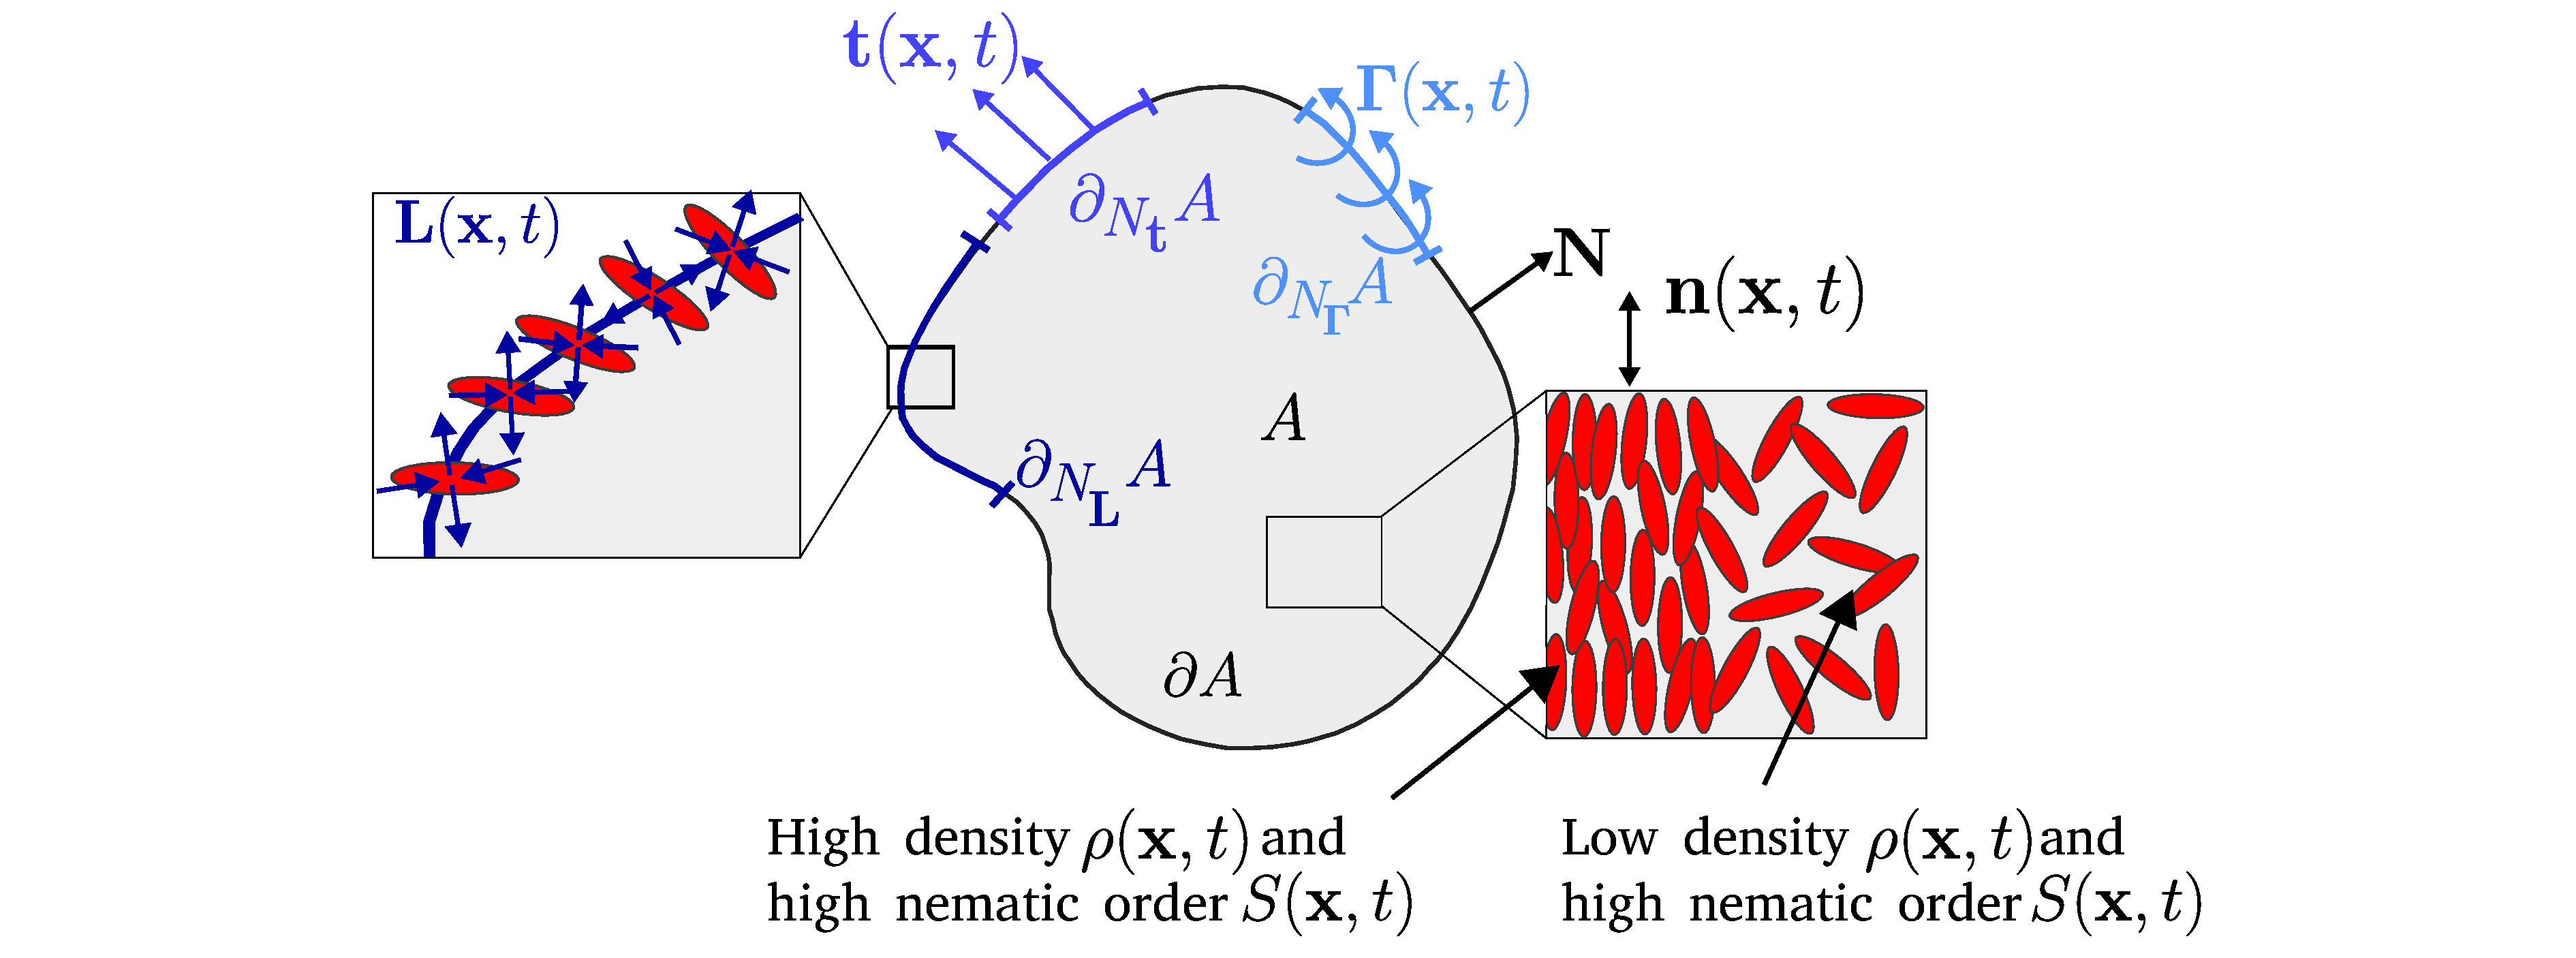
\includegraphics[width=0.9\textwidth]{fig0.pdf}
		\caption{\label{fig0}  \textbf{Schematic of a compressible active nematic gel in 2D}. The system occupies a region $A$ with boundary $\partial A$ and unit outer boundary normal $\bm{N}$. Traction $\bm{t}$, moment $\bm{\Gamma}$ and microscopic moment $\bm{L}$ act on the  boundaries $\partial_{N_{\bm{t}}} A $, $\partial_{N_{\bm{\Gamma}}} A $ and $\partial_{N_{\bm{L}}} A $, respectively. $\bm{L}$ is symmetric and traceless tensor represented with two orthogonal pairs of diverging/converging arrows of equal length and $\bm{\Gamma} = \Gamma \bm{\epsilon}$, with $\bm{\epsilon}$ the Levi-Civita tensor, is an antisymmetric tensor represented as a torque of magnitude $\Gamma$.	The active nematic system exhibits spatiotemporal variations in density $\rho(\bm{x},t)$ and the nematic order tensor $\bm{q}(\bm{x},t)$, parametrized by the nematic order parameter $S(\bm{x},t)$ and the average molecular orientation $\bm{n}(\bm{x},t)$, Eq.~(\ref{eq:nematic_tensor}), represented with a double-headed arrow.  	}
	\end{figure}
	
	\section{Governing equations of a generic active gel from Onsager's formalism} \label{sec:Onsager}
	
	\subsection{Free-energy, dissipation and power input functionals}
	
	We derive next the governing equations of an active nematic gel at low Reynolds numbers. Let $A \subset \mathbb{R}^2$ be an open set with smooth boundary $\partial A$. The unit outward normal to $\partial A$ is denoted by $\bm{N}$.  
	We assume Dirichlet boundary conditions for $\bm{v}$, $\bm{w}$ and $\widehat{\bm{q}}$ in  subsets of the boundary denoted by  $\partial_{D_{\bm{v}}} A $, $\partial_{D_{\bm{w}}} A $ and $\partial_{D_{\widehat{\bm{q}}}} A $, respectively.
	At Neumann boundaries, denoted by $\partial_{N_{\bm{t}}} A $, $\partial_{N_{\bm{\Gamma}}} A $ and $\partial_{N_{\bm{L}}} A $, we prescribe the traction vector, $\bm{t}$, the antisymmetric torque tensor, $\bm{\Gamma}$, and the generalized force power-conjugate to $\widehat{\bm{q}}$ represented by a symmetric traceless tensor, $\bm{L}$. Dirichlet and Neumann boundaries are pairwise complementary, e.g.~$\partial_{D_{\bm{v}}} A \cup \partial_{N_{\bm{t}}} A = \partial A$ and $\partial_{D_{\bm{v}}} A \cap \partial_{N_{\bm{t}}} A = \emptyset$. See Fig.~\ref{fig0} for an illustration.
	
	
	
	To derive the governing equations, we follow Onsager's variational formalism introduced in Section \ref{Ons_summ}. We postulate generic forms for the free-energy, dissipation and power input functionals as
	\begin{eqnarray}
		\mathcal{F}\left[\rho,\bm{q}\right] &=& \int_A f(\bm{q},\nabla\bm{q}) \rho dA, \label{eq:free_energy}\\
		\mathcal{D}\left[\bm{v},\widehat{\bm{q}}; \rho,\bm{q}\right] &=& \int_A d(\bm{v},\bm{d},\bm{w},\bm{\zeta},\widehat{\bm{q}};\rho,\bm{q}) \rho \,dA,\\
		\mathcal{P}\left[\bm{v},\widehat{\bm{q}}; \rho,\bm{q}\right] &=& \int_A p(\bm{v},\bm{d},\bm{w},\bm{\zeta},\widehat{\bm{q}};\rho,\bm{q}) \rho \,dA \nonumber\\
		& &~~- \int_{\partial_{N_{\bm{t}}} A} \bm{t} \cdot \bm{v} \,dl -  \int_{\partial_{N_{\bm{\Gamma}}} A} \bm{\Gamma}:\bm{w} \,dl -  \int_{\partial_{N_{\bm{L}}} A} \bm{L}:\widehat{\bm{q}} \,dl, \label{eq:power}
	\end{eqnarray}
	where $f$, $d$ and $p$ are the free-energy, dissipation, and power input densities per unit mass. The free energy depends on the state variables $\rho$ and $\bm{q}$. The dissipation and power inputs depend on process variables $\bm{v}$, $\widehat{\bm{q}}$, and might also depend parametrically on the state variables. {Examining Eq.~(\ref{eq:Jaumann}), it is clear that we could have alternatively chosen $V = \left(\bm{v}, \dot{\bm{q}}\right)$ or $V = \left(\bm{v}, \partial_t{\bm{q}}\right)$ as process variables, leading to different forms of the Euler-Lagrange equations.} 
	
	
	%%%%%%%%%%%%%%%%%%%%%%%%%%%%%%%%%%%%%%%%%%%%%%%%%%%%%%%%%%%%%%%%%%%%%%%%
	
	\subsection{Rate of change of a frame-indifferent free energy functional}\label{app:rate_of_change_energy}
	
	To write down the Rayleighian, we compute the rate of change of Eq.~(\ref{eq:free_energy}) applying Reynolds transport theorem as
	\begin{eqnarray} 
		\frac{d{\mathcal{F}}}{dt} &= \int_A \left[\partial_tf  \rho + f \partial_t{\rho} \right] dA + \int_{\partial A} f\rho \bm{v} \cdot\bm{N} ~dl = \int_A \left[\partial_tf  \rho + f \partial_t{\rho}  + \nabla\cdot\left(f\rho \bm{v}\right) \right] dA  \nonumber\\
		&=\int_A \left[\dot{f}  \rho + f \dot{\rho}  + f\rho {\rm tr}\bm{d} \right] dA. \label{eq:change_of_free_energy}
	\end{eqnarray}
	Using the chain rule, the material time derivative of $f$ can be written as
	\begin{eqnarray} 
		\dot{f} =   \frac{\partial f}{\partial q_{ab}} \dot{q}_{ab}+ \frac{\partial f}{\partial \nabla_c q_{ab}} \frac{D}{Dt} \left(\nabla_c q_{ab}\right), \label{eq:dotf}  
	\end{eqnarray}
	where we have introduced the more explicit notation $D/Dt$ for the material time-derivative when required for clarity. To further elaborate on this expression, we note that, unlike partial time and space differentiation, the material time-derivative and $\nabla$ do not commute. Indeed, the material time derivative of $\nabla \bm{q}$ is given by
	\begin{equation}
		\frac{D}{Dt} \left(\nabla_c q_{ab}\right) = \partial_t  \nabla_c q_{ab} + v_d  \nabla_d \nabla_c q_{ab},
	\end{equation}
	whereas the gradient of the material time derivative of $\bm{q}$ is
	\begin{eqnarray}
		\nabla_c \dot{q}_{ab} & = \nabla_c \left(\frac{D}{Dt} {q}_{ab}\right) = \nabla_c \partial_t   q_{ab} + \nabla_c v_d \nabla_d q_{ab} + v_d  \nabla_c \nabla_d  q_{ab} \nonumber \\ & = \frac{D}{Dt} \left(\nabla_c q_{ab}\right) + \nabla_c v_d q_{ab}  = \frac{D}{Dt} \left(\nabla_c q_{ab}\right) + d_{dc} \nabla_d q_{ab} + w_{dc} \nabla_d q_{ab}.\label{aux1}
	\end{eqnarray}
	To express $\dot{f}$ in terms of our process variable $\widehat{\bm{q}}$, we compute its gradient Eq.~(\ref{eq:Jaumann}) as
	\begin{eqnarray}
		\nabla_c \widehat{q}_{ab} =  \nabla_c \dot{q}_{ab}  + \nabla_c q_{ad} w_{db} + q_{ad}\nabla_c  w_{db}  + \nabla_c q_{db} w_{da} + q_{db} \nabla_c  w_{da}.
	\end{eqnarray}
	Combining Eq.~(\ref{aux1}) and the definition of $\bm{\zeta}$ in Eq.~(\ref{zeta}), we rewrite this expression as 
	\begin{eqnarray}
		\nabla_c \widehat{q}_{ab} = &  \frac{D}{Dt} \left(\nabla_c q_{ab}\right) + d_{dc} \nabla_d q_{ab} + w_{dc} \nabla_d q_{ab}  +  w_{db} \nabla_c q_{ad} + w_{da} \nabla_c q_{db}  \nonumber \\ & +  \left(q_{ad}\epsilon_{db}   - \epsilon_{ad} q_{db} \right)\zeta_c.
	\end{eqnarray}
	Using this expression, the material time derivative of $f$ in Eq.~(\ref{eq:dotf}) takes the form
	\begin{eqnarray} 
		\dot{f} &= &  \frac{\partial f}{\partial q_{ab}} \left(\widehat{q}_{ab}- q_{ad} w_{db}- q_{db} w_{da}\right)   + \frac{\partial f}{\partial \nabla_c q_{ab}} \bigg[ \nabla_c \widehat{q}_{ab} +  2\epsilon_{ad} q_{db}   \zeta_c \nonumber\\ && \;\;\;\;\; - d_{dc} \nabla_d q_{ab}  - w_{dc} \nabla_d q_{ab}  -  w_{db} \nabla_c q_{ad} - w_{da} \nabla_c q_{db}  \bigg], \label{eq:dotfUUUU}  
	\end{eqnarray}
	where we have used ${q}_{ab} = {q}_{ba}$ and ${\epsilon}_{ab} = -{\epsilon}_{ba}$ to simplify the term involving $\zeta_c$.
	
	The free energy density $f$ should be frame indifferent, and hence its material time derivative should vanish for any rigid body motion characterized by  $d_{ab}=0$, $\widehat{q}_{ab}=0$, and uniform but otherwise arbitrary $w_{ab}$, and hence $\zeta_c = 0$. Invoking this principle along with  Eq.~(\ref{eq:dotfUUUU}), we find that the identity
	\begin{eqnarray} 
		0 &= & \frac{\partial f}{\partial q_{ab}} \left(  q_{ad} w_{db}+ q_{db} w_{da}\right)  + \frac{\partial f}{\partial \nabla_c q_{ab}} \bigg[   w_{dc} \nabla_d q_{ab}  +  w_{db} \nabla_c q_{ad} + w_{da} \nabla_c q_{db}  \bigg],
		\label{f_frame_indiff}
	\end{eqnarray}
	should hold for all antisymmetric tensors $\bm{w}$ and for all fields $\bm{q}$. Combining Eqs.~(\ref{f_frame_indiff}) and (\ref{eq:dotfUUUU}), we finally obtain 
	\begin{eqnarray}
		\dot{f} = \frac{\partial f}{\partial q_{ab}}\widehat{q}_{ab} + \frac{\partial f}{\partial \nabla_c q_{ab}}\left( \nabla_c \widehat{q}_{ab} - d_{dc} \nabla_d q_{ab} + 2\epsilon_{ad} q_{db}  \zeta_c\right).
		\label{eq:final_rate_of_free_energy}
	\end{eqnarray}
	Plugging this expression in Eq.~(\ref{eq:change_of_free_energy}), we obtain
	\begin{eqnarray} 
		\frac{d{\mathcal{F}}}{dt} =  \int_{A}  \left[  f\frac{\dot{\rho}}{\rho}  + f  {\rm tr}\bm{d} +\frac{\partial  f}{\partial \bm{q}} : \widehat{\bm{q}}  + \frac{\partial f}{\partial \nabla_c q_{ab}}\left( \nabla_c \widehat{q}_{ab} - d_{dc} \nabla_d q_{ab} + 2\epsilon_{ad} q_{db}  \zeta_c\right) \right] \rho dA.\label{eq:dotF}
	\end{eqnarray}
	A more direct and elegant geometric derivation of this result follows from writing down the free energy in a general curvilinear coordinate system and expressing the Jaumann derivative in terms of Lie derivatives \cite{mirza2023,waleed_thesis}.
	
	Further particularizing the frame indifference condition in Eq.~(\ref{f_frame_indiff}) to uniform nematic fields ($\nabla\bm{q} = \bm{0}$)  and spin tensors of the form $\bm{w} = \bm{\epsilon}$, we obtain the condition 
	\begin{equation} 
		0 =  \frac{\partial f}{\partial q_{ac}} q_{cb} - \frac{\partial f}{\partial q_{bc}} q_{ca}.
		\label{f_frame_indiff_2}
	\end{equation}
	Similarly, considering a point where $\bm{q}=\bm{0}$ but its gradient is not, we obtain
	\begin{equation} 
		0 =  \frac{\partial f}{\partial \nabla_a q_{cd}} \nabla_b q_{cd} -  \frac{\partial f}{\partial \nabla_b q_{cd}} \nabla_a q_{cd} + 	
		2\left(\frac{\partial f}{\partial \nabla_d q_{ac}} \nabla_d q_{cb} - \frac{\partial f}{\partial \nabla_d q_{bc}} \nabla_d  q_{ca}\right).
		\label{f_frame_indiff_3}
	\end{equation}
	Equations (\ref{f_frame_indiff_2},\ref{f_frame_indiff_3}) are thus identities that should hold for all $q_{ab}$ and for all $\nabla_c q_{ab}$, and that express frame indifference of the free energy. 
	
	
	\subsection{System  Rayleighian}
	
	For clarity of our derivation, we consider the fields $\dot{\rho}$, $\bm{d}$, $\bm{w}$ and $\bm{\zeta}$ as independent variables, and enforce the kinematic and conservation relations relating them through Lagrange multipliers. Thus, the Rayleighian has the form
	\begin{eqnarray} 
		\mathcal{R}\left[\dot{\rho},\bm{v},\bm{d},\bm{w},\bm{\zeta},\widehat{\bm{q}};\rho,\bm{q}\right] = & \frac{d{\mathcal{F}}}{dt}[\dot{\rho},\bm{d},\bm{\zeta},\widehat{\bm{q}}; \rho,\bm{q}] + \nonumber
		\mathcal{D}\left[\bm{v},\bm{d},\bm{w},\bm{\zeta},\widehat{\bm{q}}; \bm{q},\rho\right] +  \\ & \mathcal{P}\left[\bm{v},\bm{d},\bm{w},\bm{\zeta},\widehat{\bm{q}}; \bm{q},\rho\right], 	\label{eq:Rayleighian}
	\end{eqnarray}
	and the governing equations can then be obtained according to Onsager's variational principle by minimizing it with respect to the extended process variables $\left(\dot{\rho}, \bm{v},\bm{d},\bm{w},\bm{\zeta},\widehat{\bm{q}}\right)$ subject to  kinematic and mass conservation constraints expressed by the functional
	\begin{eqnarray} 
		\mathcal{Q}[\varrho, & \bm{\sigma}^{\rm s}, \bm{\sigma}^{\rm a},  \bm{m}, \dot{\rho},\bm{v},\bm{d},\bm{w},\bm{\zeta},\widehat{\bm{q}};\rho,\bm{q}] =
		\int_A \left\{ \varrho  \left[\dot{\rho} + \rho{\rm tr}~\bm{d}- r\right] \vphantom{\frac{1}{2}}\right.\nonumber\\
		& +\bm{\sigma}^{\rm s} :\left[\bm{d} - \frac{1}{2}\left(\nabla \bm{v} + \left(\nabla\bm{v}\right)^T\right)\right]  %\nonumber\\& 
		+\bm{\sigma}^{\rm a} :\left[\bm{w} - \frac{1}{2}\left(\nabla \bm{v} - \left(\nabla\bm{v}\right)^T\right)\right]  \nonumber\\
		& +\left. \vphantom{\frac{1}{2}}\bm{m} \cdot \left[\bm{\zeta} - \nabla w\right] \right\}dA, \label{eq:constraints}
	\end{eqnarray}
	where $\varrho $ is the Lagrange multiplier imposing balance of mass; $\bm{\sigma}^{\rm s}$, a symmetric tensor, and $\bm{\sigma}^{\rm a}$, an antisymmetric tensor, are the Lagrange multipliers imposing the definitions of the rate-of-deformation and spin tensors; and $\bm{m}$, a vector, is the Lagrange multiplier imposing the definition of the gradient of the spin.  We thus form the  Lagrangian as 
	\begin{eqnarray} 
		\mathcal{L}[\varrho, \bm{\sigma}^{\rm s}, \bm{\sigma}^{\rm a},\bm{m},\dot{\rho},\bm{v},\bm{d},\bm{w},\bm{\zeta},\widehat{\bm{q}};&\rho,\bm{q}] = \mathcal{R}[\dot{\rho},\bm{v},\bm{d},\bm{w},\bm{\zeta},\widehat{\bm{q}};\rho,\bm{q}] \nonumber \\
		&-\mathcal{Q}[\varrho, \bm{\sigma}^{\rm s}, \bm{\sigma}^{\rm a},\bm{m}, \dot{\rho},\bm{v},\bm{d},\bm{w},\bm{\zeta},\widehat{\bm{q}};\rho,\bm{q}].	\label{eq:Lagrangian} 
	\end{eqnarray}
	
	\subsection{Balance equations and constitutive equations as optimality conditions}\label{sec_2}
	
	We examine next the first order optimality conditions. Making $\mathcal{L}$ stationary with respect to $\widehat{\bm{q}}$ and integrating by parts leads to
	\begin{eqnarray} 
		0&=&\int_A \left[ \left(\frac{\partial  f}{\partial \bm{q}} + \frac{\partial d}{\partial \widehat{\bm{q}}}+ \frac{\partial p}{\partial \widehat{\bm{q}}} \right) : \delta \widehat{\bm{q}} + \frac{\partial f}{\partial \nabla_c q_{ab}} \nabla_c \delta \widehat{q}_{ab} \right] \rho dA - \int_{\partial_{N_{\bm{L}}}A} \bm{L}:\delta\widehat{\bm{q}} dl \nonumber\\
		&=&\int_A \left[\rho \left(\frac{\partial  f}{\partial {q}_{ab}} + \frac{\partial d}{\partial \widehat{{q}}_{ab}}+ \frac{\partial p}{\partial \widehat{{q}}_{ab}} \right) - \nabla_c \left(\rho \frac{\partial f}{\partial \nabla_c {q}_{ab}} \right)   \right] \delta \widehat{{q}}_{ab}  dA \nonumber\\
		&&+ \int_{\partial_{N_{\bm{L}}}A} \left(\rho \frac{\partial f}{\partial \nabla_c {q}_{ab}} N_c -{L}_{ab}\right)\delta\widehat{{q}}_{ab} dl, \label{eq:var_q}
	\end{eqnarray}
	for all admissible traceless and symmetric variations $\delta\widehat{{q}}_{ab}$ that vanish on $\partial_{D_{\widehat{\bm{q}}}} A $. Localizing this equation, we obtain
	\begin{eqnarray} 
		\label{eq:balance_q} 
		\rho \left(\frac{\partial d}{\partial \widehat{{q}}_{ab}}+ \frac{\partial p}{\partial \widehat{{q}}_{ab}} \right) - h_{ab} = 0  \qquad & \text{in } A ,\\
		\rho \frac{\partial f}{\partial \nabla_c {q}_{ab}} N_c = {L}_{ab} \qquad & \text{on } \partial_{N_{\bm{L}}} A, \label{eq:balance_q_bd} 
	\end{eqnarray}
where we have introduced the functional derivative of the free-energy with respect to the nematic tensor
\begin{equation}
\label{nem_field}
h_{ab} = -\frac{\delta \mathcal{F}}{\delta {q}_{ab}} = -\rho \frac{\partial f}{\partial {q}_{ab}} + \nabla_c \left(\rho \frac{\partial f}{\partial \nabla_c {q}_{ab}}\right). 
\end{equation}
Equations~(\ref{eq:balance_q},\ref{eq:balance_q_bd}) express balance of generalized forces power-conjugate to $\widehat{\bm{q}}$. 
	
	Variations with respect to $\dot{\rho}$ lead to  $\varrho  = f$.
	Using this result, stationarity of $\mathcal{L}$ with respect to $\bm{d}$ provides a definition for $\bm{\sigma}^{\rm s}$:
	\begin{eqnarray} 
		\sigma^{\rm s}_{ab} = \rho\left[-\frac{1}{2} \left(\frac{\partial  f}{\partial \nabla_b q_{dc}} \nabla_a q_{dc}+ \frac{\partial  f}{\partial \nabla_a q_{dc}} \nabla_b q_{dc}\right) +  \frac{\partial  d}{\partial d_{ab}}+  \frac{\partial  p}{\partial d_{ab}}\right].
		\label{eq:sym_stress}
	\end{eqnarray}
	%where we have used the fact that variations with respect to $\dot{\rho}$ lead to $\varrho  = -f$. 
	Variations with respect to $\bm{\zeta}$ leads to
	\begin{equation}
		\label{eq:moment}
		m_c =\rho  \left(2 \epsilon_{ad} \frac{\partial  f}{\partial \nabla_c q_{ab}} q_{db} + \frac{\partial  d}{\partial \zeta_c} + \frac{\partial  p}{\partial \zeta_c}\right).
	\end{equation}
	Introducing 
	\begin{equation}
		\bm{\omega} = - \rho \left(\frac{\partial  d}{\partial \bm{w}} + \frac{\partial  p}{\partial \bm{w}}\right),
	\end{equation}
	stationarity of $\mathcal{L}$ with respect to $\bm{w}$ leads to
	\begin{eqnarray} 
		0&=\int_A \left[-\bm{\sigma}^{\rm a} :\delta\bm{w} + \frac{1}{2} {m}_c \epsilon_{ab} \nabla_c \delta w_{ab}  - \bm{\omega} :\delta \bm{w} \right] dA - \int_{\partial_{N_{\bm{L}}}A} \bm{\Gamma}:\delta\bm{w} dl\nonumber \\
		&=\int_A -\left[\bm{\sigma}^{\rm a}  + \frac{1}{2} \left(\nabla \cdot \bm{m}\right) \bm{\epsilon} +  \bm{\omega}  \right] : \delta\bm{w} \;dA + \int_{\partial_{N_{\bm{L}}}A} \left[\frac{1}{2}\left(\bm{m}\cdot\bm{N}\right) \bm{\epsilon}- \bm{\Gamma}\right]:\delta\bm{w}\; dl,
	\end{eqnarray}
for arbitrary antisymmetric variations $\delta\bm{w}$ that vanish on $\partial_{D_{\bm{w}}} A$. Localization leads to 
	\begin{eqnarray} 
		\label{sigma_a}
		\bm{\sigma}^{\rm a} + \frac{1}{2}\left(\nabla\cdot\bm{m}\right)\bm{\epsilon} +  \bm{\omega} =  \bm{0}& \qquad \text{in } A, \\ 
		\frac{1}{2}(\bm{m}\cdot\bm{N})\bm{\epsilon} =  \bm{\Gamma} & \qquad \text{on } \partial_{N_{\bm{\Gamma}}} A, 	\label{eq:balance_angular_momentum}
	\end{eqnarray}
	which is a statement of balance of angular momentum, with $\bm{m}$ playing the role of the moment in a Cosserat theory \cite{cosserat1896theorie} and $\bm{\omega}$ of body torques. Equation \eqref{sigma_a} provides a definition for $\bm{\sigma}^{\rm a}$. Combining Eqs.~\eqref{eq:balance_angular_momentum}, \eqref{eq:balance_q_bd} and the  definition for $\bm{m}$ in Eq.~\eqref{eq:moment}, we find the following boundary condition
    \begin{equation}
        \frac{1}{2} \rho \frac{\partial  (d+p)}{\partial \zeta_c} N_c \epsilon_{ab} = \Gamma_{ab} - \left(L_{ae} q_{be} - L_{be} q_{ae}\right) \qquad \text{on } \partial_{N_{\bm{L}}} A \cap \partial_{N_{\bm{\Gamma}}} A, 	\label{eq:border_xi_combined}.
    \end{equation}
	If $d$ and $p$ are independent of $\bm{\zeta}$, this equation shows that  $\bm{\Gamma}$ and $\bm{L}$ cannot be chosen independently; a  generalized force acting on nematic alignment determines the  mechanical torque at the boundary.  In this case, it is necessary that $\partial_{N_{\bm{\Gamma}}}A=\partial_{N_{\bm{L}}} A$ and $\partial_{D_{\hat{\bm{q}}}}A=\partial_{D_{\bm{w}}} A$.
	
Introducing $\bm{\sigma} = \bm{\sigma}^{\rm s} + \bm{\sigma}^{\rm a}$, the condition of stationarity of $\mathcal{L}$ with respect to $\bm{v}$ leads to 
	\begin{eqnarray} 
		0 &= \int_A \left[\bm{\sigma}:\nabla\delta\bm{v} - \delta\bm{v}\cdot\bm{f} \right]dA - \int_{\partial_{N_{\bm{t}}} A}  \bm{t} \cdot \delta\bm{v} dl \nonumber\\
		&=\int_A \left[-\nabla\cdot\bm{\sigma} - \bm{f} \right] \cdot \delta\bm{v}\;dA + \int_{\partial_{N_{\bm{t}}} A} \left(\bm{\sigma}\cdot \bm{N} -\bm{t} \right)\cdot \delta\bm{v} \;dl.	\label{eq:weak_v}
	\end{eqnarray}
	for arbitrary $\delta\bm{v}$ that vanish on $\partial_{D_{\bm{v}}} A$ and $\bm{f}=-\rho \partial  (d+p)/\partial \bm{v} $. Localizing this equation, we find the statement of balance of linear momentum in the absence of inertia
	\begin{eqnarray} 
		\nabla\cdot\bm{\sigma} + \bm{f} = \bm{0} \qquad & \text{in } A,\\
		\bm{\sigma}\cdot\bm{N} = \bm{t} \qquad & \text{on } \partial_{N_{\bm{t}}} A.	\label{eq:balance_linear_momentum}
	\end{eqnarray}
	We can hence identify $\bm{\sigma}$ as the Cauchy stress tensor, with $\bm{\sigma}^{\rm s}$ and $\bm{\sigma}^{\rm a}$  its symmetric and antisymmetric parts, and $\bm{f}$ as the body forces of dissipative and active/external origin.  Finally, variations with respect to $\varrho $, $\bm{\sigma}^{\rm s}$ and $\bm{\sigma}^{\rm a}$ lead to balance of mass (Eq.~(\ref{eq:balance_mass})) and the definitions of the rate-of-deformation and spin tensors, Eqs.~(\ref{eq:rate-of-deformation}) and~(\ref{eq:spin}).

We end this section by providing a more explicit expression for the total Cauchy stress tensor. From Eqs.~(\ref{sigma_a}) and (\ref{eq:moment}), we obtain
	\begin{eqnarray}
		{\sigma}_{ab}^{\text{a}}  & = &\nabla_c \left[\rho\left( \frac{\partial f}{\partial \nabla_c q_{bd}}q_{ad} - \frac{\partial f}{\partial \nabla_c q_{ad}}q_{bd}   \right) \right]-\frac{1}{2}\nabla_c \left( \rho \frac{\partial (  d+p)}{\partial \zeta_c}\right)\epsilon_{ab} - \omega_{ab} \nonumber \\
		 & = &  \rho \left( \frac{\partial f}{\partial \nabla_c q_{bd}} \nabla_c q_{ad} -   \frac{\partial f}{\partial \nabla_c q_{ad}} \nabla_c q_{bd}  \right) + q_{ad} \nabla_c\left( \rho  \frac{\partial f}{\partial \nabla_c q_{bd}}\right) -  q_{bd} \nabla_c\left( \rho  \frac{\partial f}{\partial \nabla_c q_{ad}}\right) \nonumber \\
		 && -\frac{1}{2}\nabla_c \left( \rho \frac{\partial (  d+p)}{\partial \zeta_c}\right)\epsilon_{ab} - \omega_{ab} \nonumber \\
		 & = &  - \frac{\rho}{2}  \left( \frac{\partial f}{\partial \nabla_b q_{cd}} \nabla_a q_{cd} -   \frac{\partial f}{\partial \nabla_a q_{cd}} \nabla_b q_{cd}  \right) + q_{ad} h_{bd} -  q_{bd} h_{ad} \nonumber \\
		 && -\frac{1}{2}\nabla_c \left( \rho \frac{\partial (  d+p)}{\partial \zeta_c}\right)\epsilon_{ab} - \omega_{ab} \label{eq::explicit_antisymmetric_stress}
\end{eqnarray}
where in the last step we have invoked frame-indifference of $f$ as expressed by Eqs.~(\ref{f_frame_indiff_2}) and (\ref{f_frame_indiff_3}) and the definition of the generalized nematic force $\bm{h}$ in Eq.~(\ref{nem_field}). Adding Eqs. (\ref{eq::explicit_antisymmetric_stress}) and 	(\ref{eq:sym_stress}), we can express the total stress as 
	\begin{eqnarray}
		\label{total_stress}
		{\sigma}_{ab} & = &  -\rho\frac{\partial  f}{\partial \nabla_b q_{dc}} \nabla_a q_{dc}  +   q_{ad}  h_{bd} - q_{bd} h_{ad}   \nonumber  \\ 
		&& + \rho \frac{\partial (d+p)}{\partial d_{ab}} + \rho \frac{\partial (d+p)}{\partial w_{ab}} -  \frac{1}{2} \nabla_c \left(\rho\frac{\partial (  d+p)}{\partial \zeta_c} \right) \epsilon_{ab}   .
	\end{eqnarray}


	\section{Standard incompressible active nematic gel} \label{sec_2_bis}
	
	Let us consider an incompressible gel (${\rm tr}\bm{d} = \nabla_a v_a =0$) with initial uniform density and $r=0$. As a result, density remains uniform and can be ignored by considering free-energy, dissipation and power input densities per unit area. %We further assume that 
	%\begin{equation}
	%f(\bm{q},\nabla\bm{q}) = f_0(\bm{q}) + \frac{L}{2}\nabla_c q_{ab} \nabla_c q_{ab},
	%\end{equation}
	%where $L>0$ is the Frank constant. 
	Because of incompressibility, the rate-of-deformation tensor is traceless and  $\bm{d}^{\rm dev} = \bm{d}$.
	
	We define a quadratic dissipation functional by its density
	\begin{equation}
		\label{diss_inc}
		d(\bm{v},\bm{d},\widehat{\bm{q}}) = \eta \vert\bm{d}^{\rm dev}\vert^2 +\frac{\eta_{\text{rot}}}{2}  \left|\widehat{\bm{q}}\right|^2+ \beta  \bm{d}^{\rm dev}:\widehat{\bm{q}}  + \frac{\gamma}{2} \left|\bm{v}\right|^2,
	\end{equation}
	where $\eta>0$ is the shear viscosity, $\eta_{\text{rot}}>0$ a viscosity parameter controlling the dissipative resistance to changes in the nematic order parameter relative to a frame that  translates and rotates with the fluid, $\beta$ captures the reciprocal drag between fluid shear and changes in nematic order, and $\gamma>0$ is a friction parameter with a substrate.
	The entropy production inequality requires non-negativity and convexity of the dissipation potential, which is satisfied whenever
	\begin{equation}
		2\eta \eta_{\text{rot}}-\beta^2\ge0.
		\label{2nd_law}
	\end{equation}
See \ref{inequality} for a related derivation of this condition. We note that there is no thermodynamic restriction on the sign of $\beta$. Physically, the natural notion that filaments align along the direction of stretching is achieved by $\beta<0$ \cite{salbreux2009}.
	
	We define power input by
	\begin{equation}
		p(\bm{d},\widehat{\bm{q}};{\bm{q}}) =\lambda \bm{q}:\bm{d}^{\rm dev} - \lambda_{\bigodot}  \bm{q} : \widehat{\bm{q}},
	\end{equation}
	which accounts for an anisotropic active tension along the nematic tensor with activity parameter $\lambda$ and a generalized active force driving further alignment with activity parameter $\lambda_{\bigodot}$.
	
	The constraint integral must include an additional term accounting for incompressibility of the form
	\begin{equation} 
		\mathcal{Q} = \ldots + 
		\int_A P ({\rm tr} \bm{d}) dA, \label{eq:constraint_}
	\end{equation}
	where $P$ is the 2D pressure (with units of surface tension) acting as a Lagrange multiplier. 
	
	Particularizing the equations in the previous section, we can write balance of generalized force conjugate to changes in nematic order, i.e.~Eq.~(\ref{eq:balance_q}), as
	\begin{equation}
		\label{bal_gen_force}
		\eta_{\text{rot}} \widehat{\bm{q}} = \bm{h} -  \beta  \bm{d}^{\rm dev} + \lambda_{\bigodot}\bm{q},
	\end{equation}
	where here density is not present in the definition of $\bm{h}$,
	\begin{equation}
		\label{nem_field2}
		h_{ab} = -\frac{\delta \mathcal{F}}{\delta {q}_{ab}} = -\frac{\partial f}{\partial {q}_{ab}} + \nabla_c  \frac{\partial f}{\partial \nabla_c {q}_{ab}}. 
			\end{equation}
	Balance of linear momentum becomes
	\begin{equation} 
		\label{bal_lin_mom}
		\gamma \bm{v} = \nabla\cdot\bm{\sigma},
	\end{equation}
where the stress tensor now accounts for the pressure  resulting from Eq.~(\ref{eq:constraint_}) and takes the form
	\begin{eqnarray}
		\label{stress_stand}
		{\sigma}_{ab}  =  -\frac{\partial  f}{\partial \nabla_b q_{dc}} \nabla_a q_{dc}  +  q_{ac} h_{cb} - q_{bc} h_{ca} + 2\eta {d}^{\rm dev}_{ab} + \beta \widehat{{q}}_{ab} + \lambda {q}_{ab} - P \delta_{ab}. 
	\end{eqnarray}
	
	In the liquid crystal literature, the dissipative coupling between strain rate and changes in nematic order appear in the stress tensor as a negative constant times $\bm{h}$ \cite{de1993}, rather than as our term $\beta \widehat{\bm{q}}$. To recover this expression, we insert the expression for generalized force balance, Eq.~(\ref{bal_gen_force}), into Eq.~(\ref{stress_stand}), to obtain
	\begin{equation}
		\label{stress_stand_2}
		{\sigma}_{ab}  = -\frac{\partial  f}{\partial \nabla_b q_{dc}} \nabla_a q_{dc}  +  q_{ac} h_{cb} - q_{bc} h_{ca} + 2\widetilde{\eta} {d}^{\rm dev}_{ab} + \widetilde{\beta} h_{ab} + \widetilde{\lambda} {q}_{ab} - P \delta_{ab},
	\end{equation}
	with effective shear viscosity $\widetilde{\eta} = \eta - \beta^2/(2\eta_{\text{rot}})$, which is positive according to Eq.~(\ref{2nd_law}), effective dissipative coupling coefficient $\widetilde{\beta}= \beta/{\eta_{\text{rot}}}$ and effective activity parameter $\widetilde{\lambda}= \lambda +  \lambda_{\bigodot} \beta/{\eta_{\text{rot}}}$. With this manipulation, the balance and constitutive equations embodied in Eqs.~(\ref{bal_gen_force}), (\ref{bal_lin_mom}) and (\ref{stress_stand_2}) agree term by term with those in \cite{julicher2018,salbreux2009}.
	
	We have thus shown that the natural expression of the stress tensor according to our theory,  Eq.~(\ref{stress_stand}), is equivalent to the the more conventional one for an incompressible model,  Eq.~(\ref{stress_stand_2}). From a physical point of view, the interpretation of $\widetilde{\beta} h_{ab}$ in Eq.~(\ref{stress_stand_2}) as a dissipative term is somewhat indirect because $h_{ab}$ depends only on the state of the system, and not on its rate-of-change. Instead, the interpretation of the dissipative stress induced by changes of nematic order relative to the fluid motion, $\beta \widehat{\bm{q}}$, is straightforward. Furthermore, Eq.~(\ref{stress_stand_2}) requires a reinterpretation of material parameters, whose physical interpretation is unambiguous in our variational approach. 
	
	
	\section{Model for a compressible active nematic gel} \label{sec_3}
	
	Having derived the generic equations for a compressible active nematic gel in Section \ref{sec_2}, here we make specific choices for free-energy, dissipation and power input to derive the governing equations for a density-dependent active nematic gel. 
	
	For the free-energy density, we assume a Landau expansion
	\begin{equation} 
		\label{eq:landau}
		f(\bm{q},\nabla\bm{q}) = \frac{1}{2}a S^2 + \frac{1}{8}b S^4 + \frac{1}{2} L \left|\nabla \bm{q}\right|^2,
	\end{equation}
	where $L>0$ is the Frank constant penalizing gradients of orientation and $a$ and $b>0$ are susceptibility parameters. For $a>0$, the susceptibility parameters penalize deviations from the isotropic state given by $S=0$. For $a<0$, the susceptibility parameters penalize deviations from anisotropic states with $S= \sqrt{-2a/b}$. 
	
	For the dissipation potential, we adapt the form of $d$ in Eq.~(\ref{diss_inc}) to a 2D compressible thin layer. To motivate our functional form, we assume that this thin layer of gel is 3D incompressible with uniform and constant volumetric density $\rho^{3D}$ and thickness $h$; hence the areal density is $\rho = \rho^{3D} h$. The 3D rate of deformation tensor $\bm{D}$
	is block-diagonal with blocks $\bm{d}$ and the out-of-plane component $D_{33}$. Since ${\rm tr}\bm{D}=0$, it follows that $D_{33} = -{\rm tr}\bm{d}$ and hence $|\bm{D}|^2 = |\bm{d}|^2 + \left(\text{tr}\bm{d}\right)^2$  \cite{salbreux2009}. As a result, the dissipation potential in the gel can be expressed as $\int_V \eta^{3D} |\bm{D}|^2 dV = \int_A \eta^{3D} |\bm{D}|^2 h dA= \int_A (\eta^{3D}/\rho^{3D}) |\bm{D}|^2 \rho dA =  \int_A \eta(|\bm{d}|^2 + \left(\text{tr}\bm{d}\right)^2)\rho dA$ with $\eta =\eta^{3D}/\rho^{3D}$. Hence, we consider the dissipation density
	\begin{equation}
		\label{eq:diss_density_example}
		d(\bm{v},\bm{d},\widehat{\bm{q}}) =  \eta \left(|\bm{d}|^2 + \left(\text{tr}\bm{d}\right)^2\right) +\frac{\eta_{\text{rot}}}{2}  \left|\widehat{\bm{q}}\right|^2+ \beta  \bm{d}^{\rm dev}:\widehat{\bm{q}}  + \frac{\gamma}{2} \left|\bm{v}\right|^2.
	\end{equation}
	Clearly, Eq.~(\ref{eq:diss_density_example}) implies that $\mathcal{D}\left[\bm{0},\bm{0}\right]=0$. The condition
	\begin{equation}
		2\eta \eta_{\text{rot}} - \beta^2 \ge 0,
		\label{diss_ineq}
	\end{equation}
	further guarantees non-negativity and convexity of the dissipation potential, \ref{inequality}. Hence, Eq.~(\ref{diss_ineq}) ensures non-negative entropy production.
	
	
	We consider the following power input density generated by out-of-equilibrium microscopic processes 
	\begin{eqnarray} 
		p(\bm{d},\widehat{\bm{q}};{\bm{q}})  & =  \lambda \textup{tr}\bm{d} + \lambda_{\rm aniso} \bm{q}:\bm{d} - (\lambda_{\bigodot}' + \rho \lambda_{\bigodot})  \bm{q} : \widehat{\bm{q}}  \nonumber \\ 
		& =   \lambda \left(\bm{I} + \kappa \bm{q}\right) : \bm{d} - \rho \lambda_{\bigodot}  \bm{q} : \widehat{\bm{q}}, 
		\label{eq:pow_density_example}
	\end{eqnarray}
	where the first term in the first line is the power of an isotropic active tension, which now makes sense because of compressibility, the second term is the power of an anisotropic active tension along the  nematic tensor, and the third term is the power of an active generalized force conjugate to changes in nematic order. In contrast to the previous section, here we expand the corresponding activity parameter up to linear order in density. The constant term $\lambda_{\bigodot}'$ has a formally equivalent effect in the governing equations as the first term in Eq.~(\ref{eq:landau}), and hence can be subsumed in susceptibility parameter $a$.  For this reason we consider $\lambda_{\bigodot}'= 0$ in the second line, where  we group active tensions in a single term by defining the tension anisotropy parameter $\kappa=\lambda_{\rm aniso}/\lambda$. For $\lambda_{\bigodot}>0$, nematic activity tends to further increase alignment.
	
	
	With the free-energy, dissipation and power-input functions in Eqs.~(\ref{eq:landau},\ref{eq:diss_density_example},\ref{eq:pow_density_example}), Onsager's variational formalism developed in Section~\ref{sec:Onsager} yields the following generalized force balance equation
	\begin{equation}  \label{first_govern}
		\eta_{\text{rot}} \widehat{\bm{q}} + \beta \bm{d}^{\rm dev} + (2a + b S^2)  \bm{q} - L \left(\Delta \bm{q} +   \nabla\bm{q} \cdot \frac{\nabla \rho}{\rho} \right) - \rho\lambda_{\bigodot} \bm{q} = \bm{0}.
	\end{equation}
	This equation shows that $2a-\rho \lambda_{\bigodot}$ can be interpreted as an effective susceptibility coefficient, which if negative, triggers spontaneous ordering. 
	
	Balance of linear momentum takes the form
	\begin{equation}
		\label{eq:balance_forces_linear}
		\nabla\cdot\bm{\sigma} = \rho \gamma \bm{v},
	\end{equation}
	where the stress tensor is the sum of its symmetric component
	\begin{equation}
		\sigma^{\rm s}_{ab} = \rho \left[2\eta  (d_{ab}+d_{cc} \delta_{ab}) + \beta  \widehat{q}_{ab}  + \lambda \left(\delta_{ab} + \kappa q_{ab}\right) -L\nabla_a q_{cd} \nabla_b q_{cd}\right],
	\end{equation}
	and its antisymmetric component 
	\begin{equation}
		\sigma^{\rm a}_{ab} = L \left[\nabla_c \rho \left( q_{ad} \nabla_c q_{db}  - q_{bd} \nabla_c q_{da}  \right)   + \rho  \left(q_{ae}\Delta q_{be}  -q_{be}  \Delta q_{ae}  \right) \right].
	\end{equation}
	For the boundary conditions, we either consider examples where $\bm{t}$, $\bm{\Gamma}$ and $\bm{L}$ are zero, leading to homogeneous Neumann boundary conditions, or examples where $\bm{v}$ and $\widehat{\bm{q}}$ are fixed, leading to Dirichlet boundary conditions. For the right-hand side of Eq.~(\ref{eq:balance_mass}), we consider a polymerization rate $k_p$, a depolymerization rate proportional to $\rho$ and given by $-k_d \rho$, and Fickian diffusion with diffusivity $D$,
	\begin{equation} \label{last_govern}
		\dot{\rho} + \rho {\rm tr}~\bm{d} = k_p - k_d \rho + D \Delta \rho.
	\end{equation}
	
	We end this section by briefly discussing how this model can lead to patterns of nematic order. The conventional mechanisms for nematic ordering are driven by the free energy $f$, e.g.~as a result of the excluded volume effects in the mixing entropy of elongated particles \cite{Onsager_shape,de1993,D0SM01733G}. The model presented here can account for this mechanism by considering $a<0$, as in the numerical study in Section \ref{ex2}, possibly in a density-dependent manner. However, as illustrated by the numerical study in Section \ref{ex1} and in \cite{mirza2022}, nematic order can also arise through an active mechanism according to which self-reinforcing convergent flows produce velocity gradients and density accumulation  that increase order as a result of terms $\beta \bm{d}^{\rm dev}$ and $- \rho\lambda_{\bigodot} \bm{q}$ in Eq.~\ref{first_govern}.
	
	
	
	
	\section{Finite element formulation} \label{sec_4}
	
	
	The governing Eqs.~(\ref{first_govern}-\ref{last_govern}) of the proposed model are non-linear and involve tight couplings between nematic, velocity and density fields. For this reason, a solution of the governing equations in arbitrary geometries and boundary conditions cannot be obtained by analytical means. Here, we develop a finite element computational approach building on Onsager's variational formalism. In this setting, numerical space discretization is straightforward and follows from performing extremization of the Lagrangian in a constrained functional space given by the finite element approximation of the process variable fields. The resulting stationarity conditions represent the discretized weak form of the governing equations. For time discretization, we resort to the implicit Euler method. 
	
	\subsection{Weak form of the governing equations}
	
	In Eqs.~(\ref{eq:Rayleighian}) and~(\ref{eq:Lagrangian}), we have expressed the Rayleghian and the Lagrangian in terms of the independent variables $\dot{\rho},\widehat{\bm{q}},\bm{v},\bm{d},\bm{w}$ and $\bm{\zeta}$ to derive the governing equations in the most physically meaningful form. However, to derive an Eulerian finite element method, it is more convenient to  consider $\partial_t{\bm{q}}$ and $\bm{v}$ as the sole process variables. From the first expression in Eq.~(\ref{eq:change_of_free_energy}), applying the chain rule to compute $\partial_t f$ and using Eq.~(\ref{eq:balance_mass}), we can express the rate of change of the free energy as
	\begin{eqnarray} 
		\frac{d{\mathcal{F}}}{dt}\left[\partial_t\bm{q},\bm{v};\rho,\bm{q}\right] = &  \int_A \left\{ \rho \frac{\partial f}{\partial \bm{q}} : \partial_t \bm{q} + \rho \frac{\partial f}{\partial \nabla_c {q}_{ab}}  \nabla_c \partial_t {q}_{ab} + f \left[r-\nabla\cdot\left(\rho\bm{v}\right)\right] \right\}dA  \nonumber\\ 
		&  +  \int_{\partial_{N}A} f\rho \bm{v} \cdot\bm{N} dl. \label{eq:discrete_free_energy}
	\end{eqnarray}
	For the dissipation and power potentials, we directly substitute the definitions of $\bm{w}$ and $\bm{\zeta}$ as a function of gradients of $\bm{v}$ and use Eq.~(\ref{eq:Jaumann}) to write $\widehat{\bm{q}}$ in terms of $\partial_t \bm{q}$ and $\bm{v}$, formally leading to functionals of the form $\mathcal{D}[\partial_t\bm{q},\bm{v};\rho,\bm{q}]$ and $\mathcal{P}[\partial_t\bm{q},\bm{v};\rho,\bm{q}]$.
	%\begin{eqnarray}   \label{eq:discrete_dissipation}
	%	\mathcal{D}[\partial_t\bm{q},\bm{v};\rho,\bm{q}] = \int_A d\left(\partial_t\bm{q},\bm{v};\bm{q}\right)  \rho dA,
	%\end{eqnarray}
	%\begin{eqnarray}  \label{eq:discrete_power}
	%	\mathcal{P}[\partial_t\bm{q},\bm{v};\rho,\bm{q}] = \int_A p\left(\partial_t\bm{q},\bm{v};\bm{q}\right)  \rho dA.
	%\end{eqnarray}
	Combining these functionals, the Rayleighian can be expressed as
	\begin{equation}  \label{eq:ray_discrte}
		\mathcal{R}[\partial_t\bm{q},\bm{v};\rho,\bm{q}] = \frac{d{\mathcal{F}}}{dt}[\partial_t\bm{q},\bm{v};\rho,\bm{q}]+ \mathcal{D}[\partial_t\bm{q},\bm{v};\rho,\bm{q}]+ \mathcal{P}[\partial_t\bm{q},\bm{v};\rho,\bm{q}].
	\end{equation}
	Onsager's variational principle then provides an alternative form of the governing equations by minimizing this Rayleighian with respect to $\partial_t \bm{q}$ and $\bm{v}$.  Minimization with respect to  $\partial_t\bm{q}$ leads to 
	\begin{eqnarray}
		0&=\delta_{\partial_t \bm{q}} \mathcal{R} 
		&=  \int_A  \bigg[ \left(\frac{\partial  f}{\partial \bm{q}} +   \frac{\partial (d+p)}{\partial \widehat{\bm{q}}}  \right):\bm{p} + \frac{\partial f}{\partial \nabla_c {q}_{ab}}  \nabla_c  {p}_{ab} \bigg]\rho dA -   \int_{\partial_{N_{\bm{L}}}A} \bm{L}:\bm{p} dl, \label{eq:weak_q_disc}
	\end{eqnarray}
	where $\bm{p}$ is an arbitrary variation of $\partial_t \bm{q}$, and hence a traceless and symmetric second order tensor. Integration by parts of this weak form to obtain the corresponding Euler-Lagrange equations is not required for the finite element discretization. 
	
	Minimization with respect to $\bm{v}$ leads to
	\begin{eqnarray}
		\bm{0}=\delta_{\bm{v}} \mathcal{R}=   ~\int_A &\left\{-\frac{ f}{\rho} \nabla \cdot \left(\rho\bm{u}\right) + \frac{\partial ( d+ p)}{\partial \bm{v}} \cdot\bm{u}    \right.  
		+ \left[\frac{\partial ( d+ p)}{\partial \bm{d}} + \frac{\partial ( d+ p)}{\partial \bm{w}}\right] : \nabla\bm{u}\nonumber\\
		&+ \left. \frac{\epsilon_{ab}}{2} \frac{\partial ( d+ p)}{\partial {\zeta}_c} \nabla_c \nabla_b {u}_a + \frac{\partial ( d+ p)}{\partial \widehat{\bm{q}}} : \delta_{\bm{v}} \widehat{\bm{q}} \right\} \rho dA 
		+   \int_{\partial A} f\rho \bm{N}\cdot\bm{u}\,dl	
		\nonumber\\
		& - \int_{\partial_{N_{\bm{t}}} A} \bm{t} \cdot \bm{u} \,dl -  \int_{\partial_{N_{\bm{\Gamma}}} A} \bm{\Gamma}:\nabla\bm{u} \,dl -  \int_{\partial_{N_{\bm{L}}} A} \bm{L}:\delta_{\bm{v}} \widehat{\bm{q}} \,dl
		\label{eq:weak_v_disc}
	\end{eqnarray}  
	where $\bm{u}$ is an arbitrary variation of $\bm{v}$. The variation of the Jaumann derivative of the nematic order tensor with respect to velocity is given by $\delta_{\bm{v}} \widehat{{q}}_{ab}=  {u}_c\nabla_c{q}_{ab} + \frac{1}{2}\left({q}_{ac} {\epsilon}_{cb} -{\epsilon}_{ac}{q}_{cb} \right) {\epsilon}_{ef}\nabla_f{u}_e$. 
	
We note that, although not written here, non-homogeneous Dirichlet boundary conditions on $\partial_{D_{\bm{w}}} A $ and $\partial_{D_{\widehat{\bm{q}}}} A $ would need to be explicitly enforced in the formulation presented here, e.g.~through Lagrange multipliers, because constraints on $\widehat{\bm{q}}$ and $\bm{w}$ depend on  $\partial_t \bm{q}$ and $\bm{v}$ in a non-trivial manner. 
	
The equivalence between Eq.~(\ref{eq:weak_v_disc}) and the form of balance of linear momentum found earlier in Eq.~(\ref{eq:weak_v}) is not obvious even if both of these equations encode the same physics. In \ref{equivalence}, we explicitly show this equivalence. 

For balance of mass, we consider the weak form of Eq.~(\ref{eq:balance_mass}) by  multiplying by an arbitrary test function $\delta\rho$, integrating, and applying the divergence theorem to the diffusive term to obtain
	\begin{eqnarray}
		\int_A \left \{\left(  \frac{\partial \rho}{\partial t} +  \nabla \cdot (\rho \bm{v}) - k_p  +\rho k_d\right) \delta \rho  + D\nabla \rho \cdot \nabla \delta \rho \right \} dA \nonumber \\ 	-  \int_{\partial A} D  \nabla \rho \cdot \bm{N} \delta \rho  dl  = 0.  \label{eq:weak_mass}
	\end{eqnarray}
	The boundary integral is dealt with by either prescribing the diffusive flux across the boundary or by considering $\delta\rho=0$ in parts of the boundary where $\rho$ is fixed.
	
	\subsection{Space discretization}
	
	
	We discretize fields in space following a typical finite element approximation based on a mesh with $N$ vertices. Each vertex or node $I$ of the mesh has an associated basis function $B_I(\bm{x})$. The choice of the type of basis function depends on the required regularity. The weak form in Eq.~(\ref{eq:weak_v_disc}) contains second-order derivatives of $\bm{u}$, and hence should require basis functions with at least square-integrable second order derivatives. However, since in our model $\partial ( d+ p) / \partial \bm{\zeta} = \bm{0}$, only first order derivatives of $\bm{u}$ (and $\bm{v}$) appear, and hence a conventional finite element discretization with $C^0$ continuity can be used. The density field is discretized as
	\begin{equation}
		\rho(\bm{x},t) = \sum_{I=1}^N \rho_I(t) B_I(\bm{x}), \label{eq:shape_func}
	\end{equation}
	where $\rho_I(t)$ is the $I-$th nodal coefficient at time $t$. Analogously, we have 
	\begin{equation}
		\bm{v}(\bm{x},t) = \sum_{I=1}^N\bm{v}_I(t) B_I(\bm{x}),
	\end{equation}
	where the nodal degrees of freedom are vectors. 
	We represent the traceless and symmetric nematic tensor field as
	\begin{equation}
		\bm{q}(\bm{x},t) = \left(\begin{array}{cc}
			q_1(\bm{x},t) & q_2(\bm{x},t)\\
			q_2(\bm{x},t) & -q_1(\bm{x},t)
		\end{array}\right),
	\end{equation}
	and discretize its components as
	\begin{equation}
		q_1(\bm{x},t) = \sum_{I=1}^N q_{1I} (t) B_I(\bm{x}), \qquad  q_2(\bm{x},t) = \sum_{I=1}^N q_{2I} (t) B_I(\bm{x}).
	\end{equation}
	Thus, we have 5 degrees of freedom per node, namely $\rho_I, v_{1I}, v_{2I}, q_{1I}$ and $q_{2I}$.
	
	To discretize Eq.~(\ref{eq:weak_q_disc}), we express variations $\bm{p}$ as linear combinations of the following traceless symmetric tensors 
	\begin{equation}
		\left(\begin{array}{cc}
			B_I(\bm{x}) & 0\\
			0 & -B_I(\bm{x})
		\end{array}\right) \qquad \mbox{and} \qquad  \left(\begin{array}{cc}
			0 & B_I(\bm{x})\\
			B_I(\bm{x}) & 0
		\end{array}\right),
	\end{equation}
	for all $I$.  Using the space-discretized nematic tensor and the variations defined above, the discretized form of balance of generalized force conjugate to nematic order in Eq.~(\ref{eq:weak_q_disc}) becomes a set of $2N$  algebraic equations. For the balance of linear momentum, Eq.~(\ref{eq:weak_v_disc}), we consider variations of velocity $\bm{u}$ to be linear combinations of $[B_I(\bm{x})\;\; 0]^T$ and $[0\;\; B_I(\bm{x})]^T$ to obtain $2N$ additional algebraic equations. Finally, for the balance of mass, Eq.~(\ref{eq:weak_mass}), we consider $\delta\rho$ to be linear combinations of $B_I(\bm{x})$ to obtain $N$ equations. We note that when advection dominates in Eq.~(\ref{eq:weak_mass}), such a Galerkin approach, in which $\delta\rho$ are discretized with the same basis functions as $\rho$, leads to numerical instabilities. In our implementation, we check the condition for stability and stabilize the numerical formulation using the SUPG method if required \cite{donea2003}.  Hence, we obtain a set of $5N$ differential-algebraic equations involving $\rho_I$, $v_{1I}$, $v_{2I}$, $q_{1I}$, $q_{2I}$, and the time-derivatives of the density and nematic degrees of freedom.
	
	
	\subsection{Time discretization and solution method}
	
	
	%Together,  Eqs.~(\ref{eq:weak_mass},\ref{eq_week_1}-\ref{eq_week_4}) constitute a differential-algebraic system of $5N$ coupled equations. 
	We discretize these equations in time using a non-uniform grid of time-steps that we denote by the superindex $[\text{n}]$. We denote by $\rho^{[\text{n}]}_I$, $\bm{q}^{[\text{n}]}_I$, and $\bm{v}^{[\text{n}]}_I$ the nodal coeficients at the $n-$th time-step, and consider  a backward Euler approximation, according to which we evaluate all fields in Eqs.~(\ref{eq:weak_q_disc}-\ref{eq:weak_mass}) at step $[\text{n}]$ and approximate time-derivatives as $\partial_t \rho_I^{[\text{n}]} = (\rho^{[\text{n}]}_I-\rho^{[\text{n-1}]}_I)/\Delta t^{[\text{n}]}$, $\partial_t \bm{q}_I^{[\text{n}]} = (\bm{q}^{[\text{n}]}_I-\bm{q}^{[\text{n-1}]}_I)/\Delta t^{[\text{n}]}$. This leads to a set of nonlinear algebraic equations that we solve with Newton-Raphson's method. 
	We test our implementation by performing space and time convergence numerical experiments, finding the expected convergence rates, see ~\ref{appendix_grid}.
	
	\section{Computational studies of active nematodynamics}\label{sec_5}
	
	\subsection{Cell wound healing}
	\label{ex1}
	
	The dynamical assembly of a contractile ring is essential to close holes and tears formed in the cortex of the Xenopus egg, as systematically examined with laser ablation experiments \cite{benink2000,mandato2001}. Ablation triggers a localized stimulus increasing myosin-II activity at the edge of the wound. A more contractile region in the actomyosin gel produces a gradient in active tension driving long-range cortical flows. The interplay between actin flow and enhanced myosin activity leads to the assembly of a ring made of a dense network of interconnected F-actin bundles, myosin-II and other actin-binding proteins. Inside the contractile ring, the network is aligned parallel to the boundary of the wound. This contractile ring leads to wound closure by the purse-string mechanism \cite{Alice2008}.
	
	
	\begin{figure}[t]
		\centering
		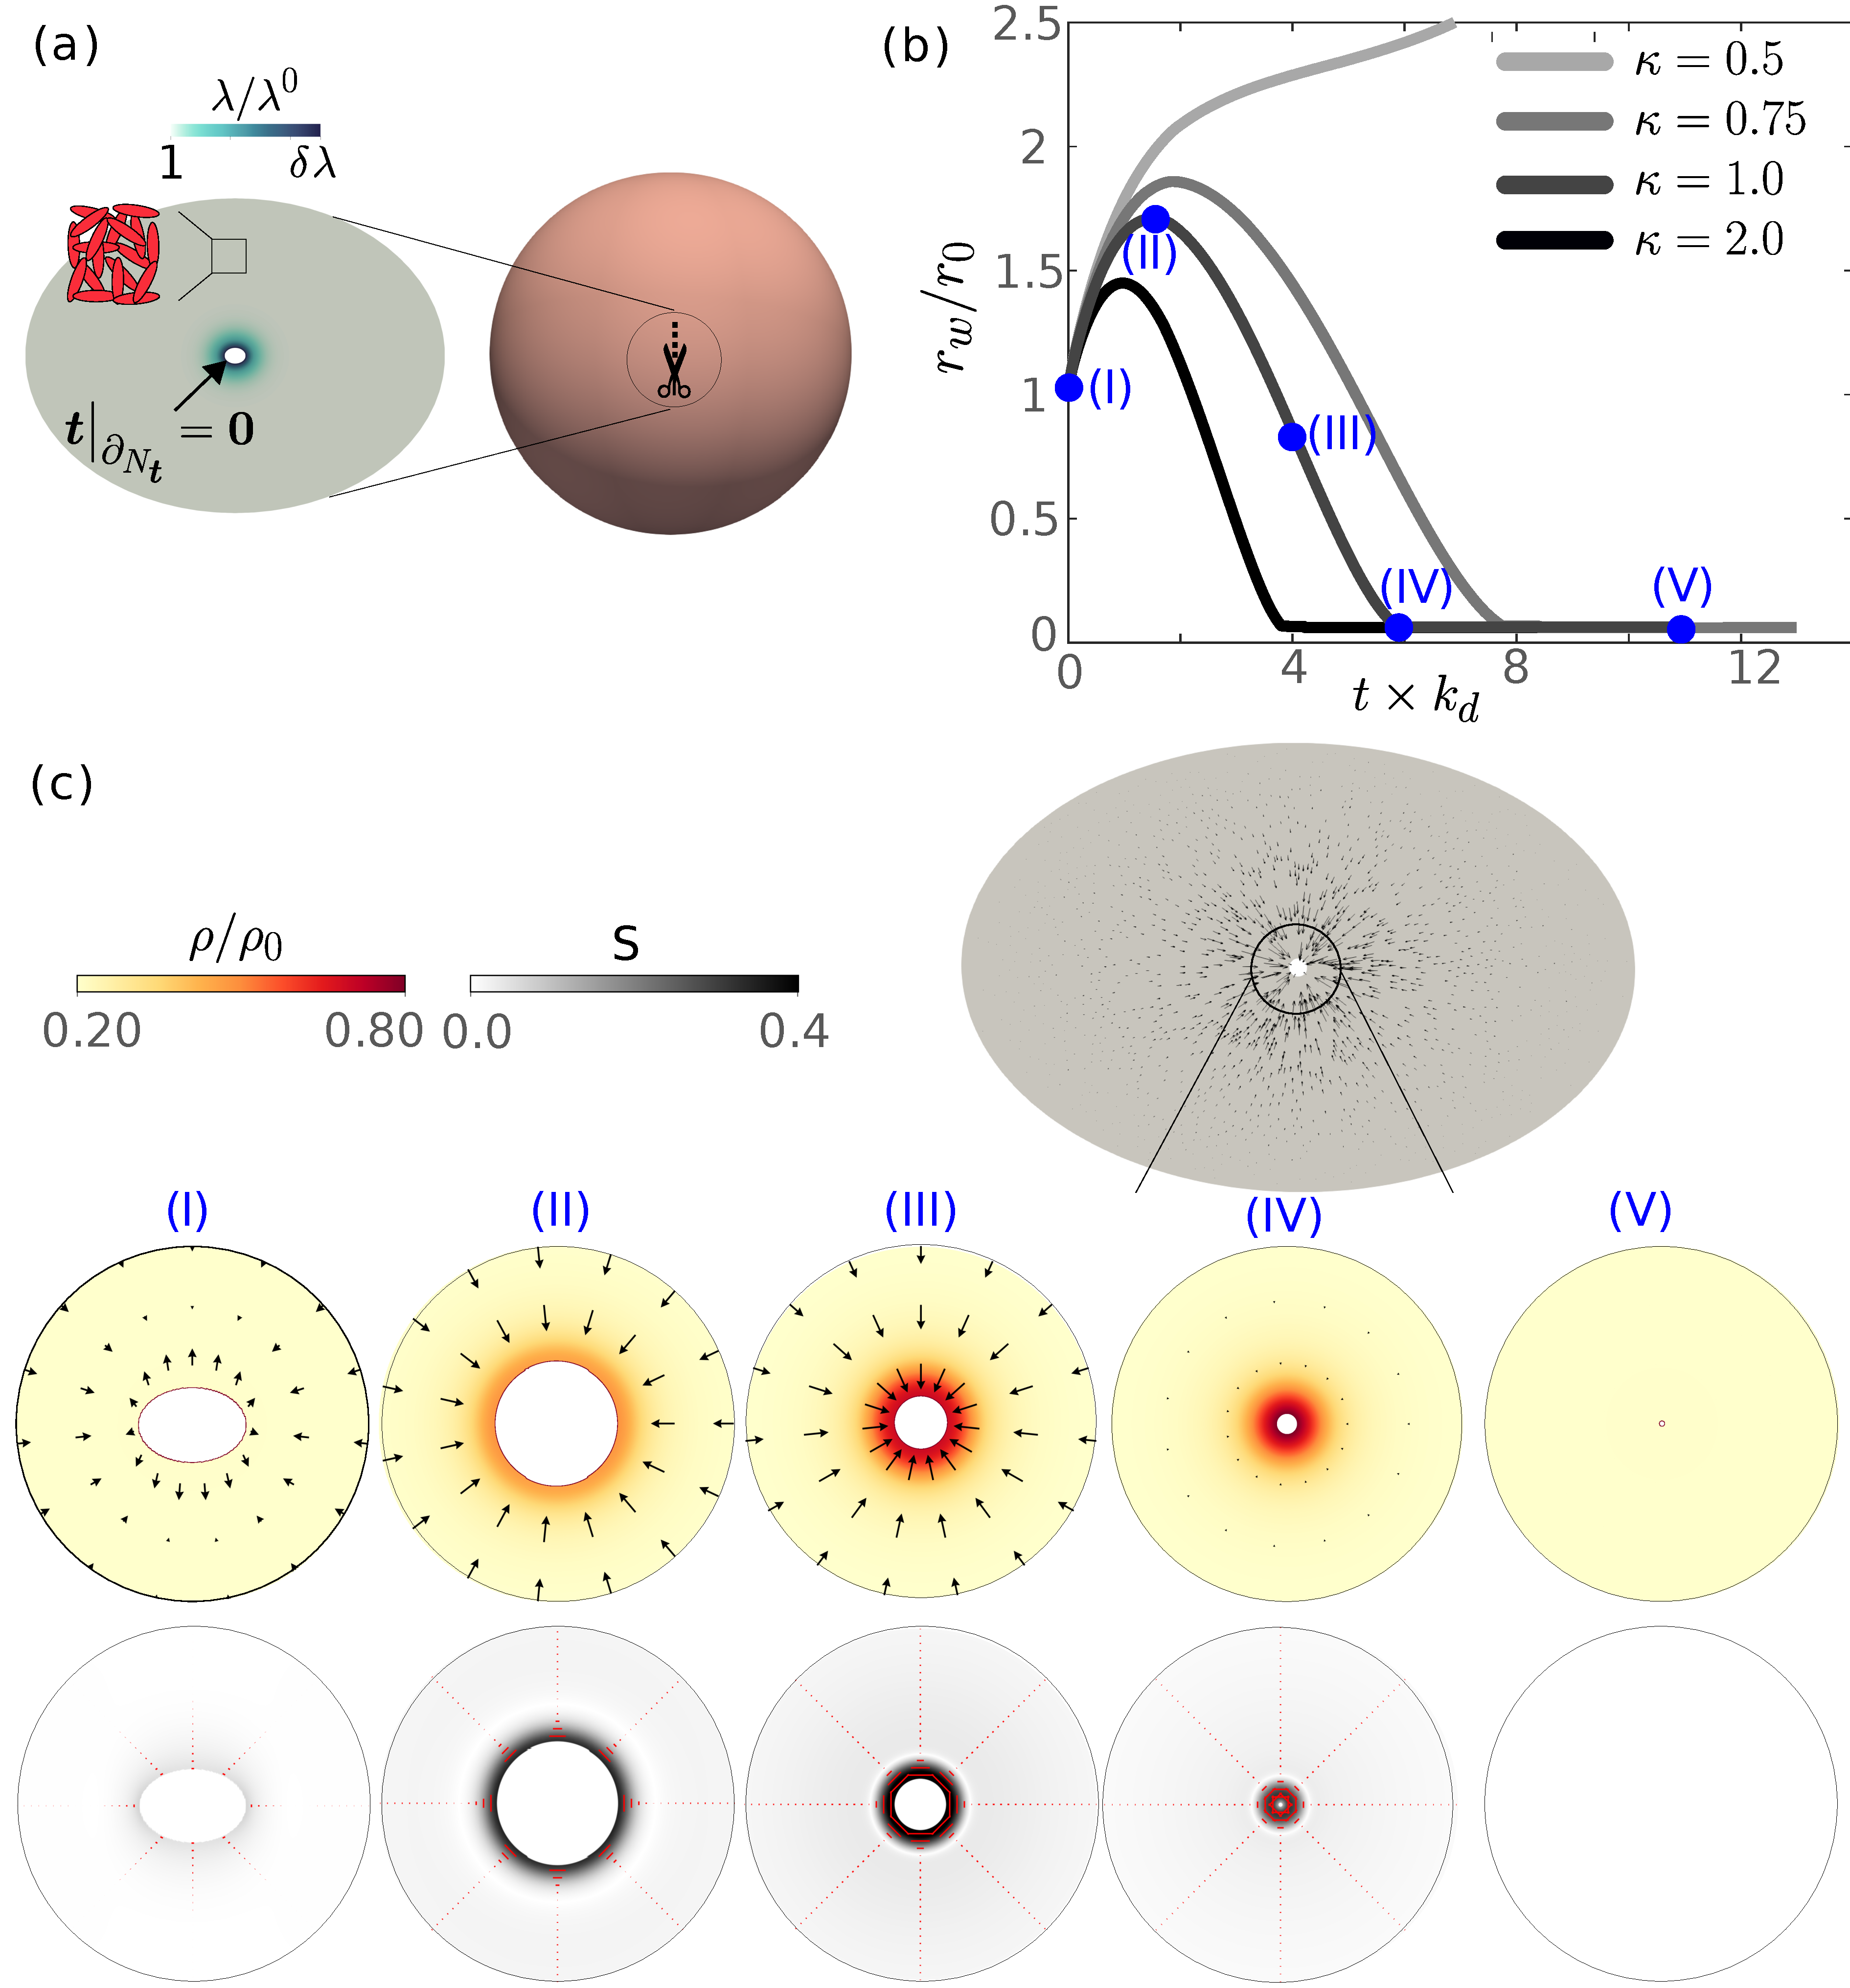
\includegraphics[width=0.75\textwidth]{fig1.pdf}
		\caption{\label{sec_1_chap_3_fig_1} \textbf{Simulation of the process of wound healing}. (a) Schematic of cell wound healing. (b) Normalized wound size, where $r_w$ is the characteristic wound size and $r_0$ the minor axis of the initial wound, as a function of dimensionless time for different values of active tension anisotropy $\kappa$. (c) Snapshots of flow and density fields (top) and nematic field (bottom, segments denote nematic direction and colormap indicates $S$) close to the wound. See also Movie~1.}	
	\end{figure}
	
	Here, we examine the self-organization of the contractile ring using the active nematic gel theory presented in Section \ref{sec_3} and study conditions leading to wound closure. The model setup is  illustrated in Fig.~\ref{sec_1_chap_3_fig_1}(a). We make the following assumptions. We ignore the curvature of the cell and consider a  planar patch of actin cytoskeleton. The characteristic size of the domain $ \ell_0$ is much larger than any inherent length-scales of the model such as the hydrodynamic length scale $\ell_s=\sqrt{\eta/\gamma}$ or the nematic correlation length scale $\ell_p=\sqrt{L/|2a-\rho_0\lambda_{\bigodot}|}$. This assumption implies that at distances greater than $\ell_s$ and $\ell_p$, the effect of the ablated region on the system is negligible. We represent the ablated region as an ellipse with aspect ratio $1.5$ and  minor axis $r_0$. We denote the characteristic wound size with $r_w(t)$ calculated as the minimum distance from the edge of the wound to its centroid. To reflect an enhanced activity around the ablated region, we set the parameters that control active tension to
	\begin{eqnarray} 
		\lambda(\bm{x},t)=  \lambda^{0} \left( 1+  \delta \lambda\text{e}^{-r(\bm{x},t)/w}  \right), \;\;\;\;\mbox{and}\;\;\;\;
		\lambda_{\bigodot}(\bm{x},t)=  \lambda^{0}_{\bigodot} \left( 1+   \delta \lambda\text{e}^{-r(\bm{x},t)/w}  \right), \label{eq:over_activity_1}
	\end{eqnarray}
	where $r(\bm{x},t)$ is the distance between point $\bm{x}$ and its closest point projection on the boundary of the wound at time $t$.  In Eq.~(\ref{eq:over_activity_1}), $\lambda^0$ and  $\lambda_{\bigodot}^0$ are the base activity parameters and  $\delta \lambda$ sets the amplitude of the enhanced activity, which decays with the distance to the wound edge. We consider the width of the over-activity region $w$ to be larger than $\ell_p$ and smaller than $\ell_s$. 
	
	The initial conditions are those of a uniform, quiescent and isotropic gel in its steady-state, and hence we make sure that the effective susceptibility $2a -  \rho_0\lambda_{\bigodot}$ is positive. All material parameters are given in Table~\ref{modal_parameters_cell_healing}. We assume traction-free boundary conditions at the wound edge. To track changes of domain shape during wound closure, we adopt an updated  Lagrangian approach; at each time-step, we update the nodes of the mesh following $\bm{x}^{[\text{n}]}  = \bm{v}^{[\text{n}]}\Delta t^{[\text{n}]}+ \bm{x}^{[\text{n-1}]}$. To maintain the mesh quality during this Lagrangian flow, after updating the nodal coordinates of the mesh, we perform reparametrization of the mesh while keeping the boundary fixed if the local element distortion  exceeds a given threshold. The reparametrization of the domain is performed using a customized version of the \textit{vtkvmtkPolyDataSurfaceRemeshing} class of the Vascular Modeling Toolkit (VMTK) \cite{antiga2008}. Once the deformed mesh is reparameterized, density and nematic tensor fields are mapped from the deformed mesh to the reparameterized mesh. To do so, we first perform a closest-point projection (using the function $\textit{FindClosestPoint}$ of the $\textit{vtkCellLocator Class}$ from the VTK library \cite{schroeder2003}) to establish a one-to-one mapping between material points in these two meshes. Then, the fields $\bm{q}$ and $\rho$ are projected in the reparametrized mesh by a least-squares procedure. 
	
	
	
	\begin{figure}[t]
		\centering
		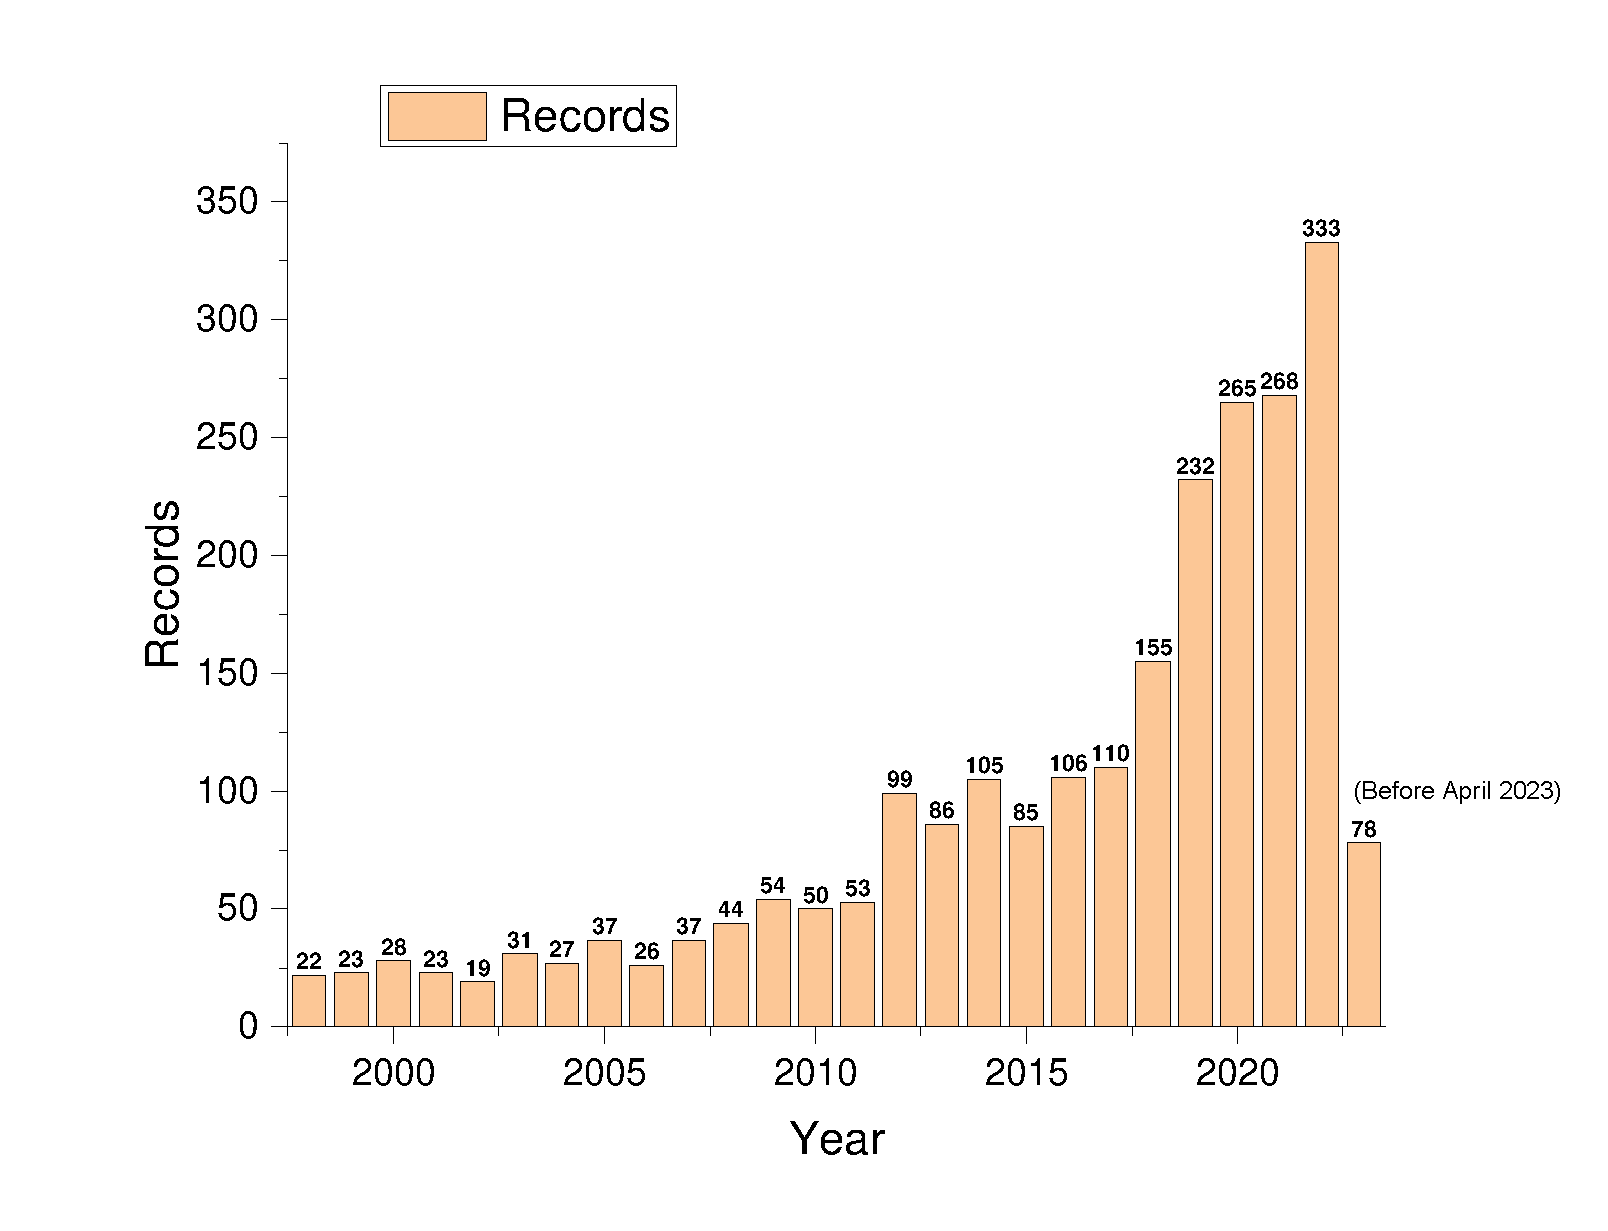
\includegraphics[width=0.75\textwidth]{fig2.pdf}
		\caption{\label{sec_1_chap_3_fig_2}  \textbf{Effect of the flow-aligning parameter $\beta$ and nematic activity $\lambda_{\bigodot}$ on the healing dynamics}. Normalized wound size  $r_w$ as a function of time for different choices of parameters. The snapshots (I-III) show the nematic organization at a given wound size for different $\lambda_{\bigodot}$. The nematic field is represented by a color map for $S$ and by red segments, whose direction indicates the nematic orientation and whose size is proportional to $S$.}
	\end{figure}
	
	We first examine the role of $\kappa$, characterizing the anisotropy of active tension, as shown in Fig.~\ref{sec_1_chap_3_fig_1}(b). To illustrate the process of wound healing according to our model, we first focus on the curve corresponding to $\kappa=1.0$ with five snapshots I to V showing wound shape, density, velocity and nematic order, Fig.~\ref{sec_1_chap_3_fig_1}(c).  At time-point I, we impose a local increase of activity following Eq.~(\ref{eq:over_activity_1}). At this instant and due to tension in the active gel, the wound edge retracts away from the center increasing the size of the wound. At the same time, a centripetal actin flow driven by the gradient in active tension develops in a region of size commensurate to the hydrodynamic length. This convergent flow locally densifies the gel close to the edge of the wound, which further reinforces contractility and  flow towards the edge. The centripetal flow rapidly decreases at the wound edge (it actually changes sign between instants I and II), generating a strong velocity gradient. Due to the flow-alignment effect associated to $\beta<0$, this velocity gradient increases nematic order near the edge parallel to the edge, whereas far away nematic order is weak with alignment perpendicular to the wound edge. The localized density and nematic order in the wound edge mobilize the generalized active nematic force $-\rho\lambda_{\bigodot}\bm{q}$ further driving order. In summary, local edge overactivity along with the traction-free boundary condition lead to the self-assembly of a dense contractile bundle with high alignment. Since here $\kappa >0$, this ring is highly contractile, creating a Laplace-like force in the curved wound edge, which tends to make it circular and overcomes cortical surface tension to close the wound, Fig.~\ref{sec_1_chap_3_fig_1}(III,IV). As the wound closes, the architecture of the contractile ring is stabilized by the interplay of cytoskeletal self-enhancing flows, flow-induced alignment, active alignment, diffusion, and  turnover. This leads to a robust process of wound healing. When the size of the wound is very small relative to all other length-scales of the problem, we consider that the wound has closed and hence set the overactivity signal $\delta \lambda=0$. As a consequence,  the self-reinforcing flows rapidly decrease and  the contractile ring disassembles as cytoskeletal density reduces due to turnover (V). Hence, following a largely self-organized process of wound healing, the cortex recovers homeostasis. See Movie 1 for an illustration. A parametric sweep for different values of $\kappa$ shows that $\kappa$ needs to be sufficiently high for wound closure, Fig.~\ref{sec_1_chap_3_fig_1}(b).
	
	
	We then examined the effect of $\lambda_{\bigodot}$ and $\beta$ on wound healing,  Fig.~\ref{sec_1_chap_3_fig_2}. A higher value of $\lambda_{\bigodot}$ self-organizes a contractile ring with a higher nematic order on a shorter time scale. This leads to a quicker inhibition of  wound opening and of  reversal of  boundary motion. Contrasting with this strong effect, the flow-aligning parameter $\beta$ has a milder and more subtle effect. A higher $\beta$ promotes the fast formation of the contractile ring, but also aligns radially the network far away, see inset, counteracting the effect of the ring. Close to the threshold between wound closing and opening, changes in $\beta$ can have a dramatic effect on the dynamics, see blue curves.
	
	
	\subsection{Defects in a confined colony of spindle-shaped cells}
	\label{ex2}
	
	Having examined a situation where nematic order has an active origin linked to self-reinforcing flows, we turn now to a more conventional situation in which ordering is driven by $a<0$. Elongated spindle-shaped contractile cells such as myoblasts or fibroblasts exhibit long-range nematic order in circular confined dense cultures \cite{duclos2014,guillamat2020} due to their tendency to mutually align parallel with each other \cite{elsdale1968}. Cells confined in these circular domains tend to align parallel or perpendicular to the boundary \cite{guillamat2020}.
	Because of this boundary alignment and the spontaneous tendency to nematic ordering, the net charge of the topological defects in the colony is $+1$, as required by the Poincar\'{e}-Hopf theorem \cite{jubin2009}. This is satisfied by the generation of one or more pairs of topological defects with charge $\pm 1/2$.
	%This leads to disruption in the nematic field by self-organization of $\pm 1/2$  topological defects.
	Because nematic order controls the anisotropy of active stresses in the cell monolayer, topological defects actively move and may lead to a variety of out-of-equilibrium behaviors. 
	Depending on the size of the geometrical confinement with respect to the characteristic lengths of the system, self-organized flows and motion of defects are either absent \cite{duclos2014}, spiral or turbulent-like \cite{norton2018}. 
	
	\begin{figure}[t]
		\centering
		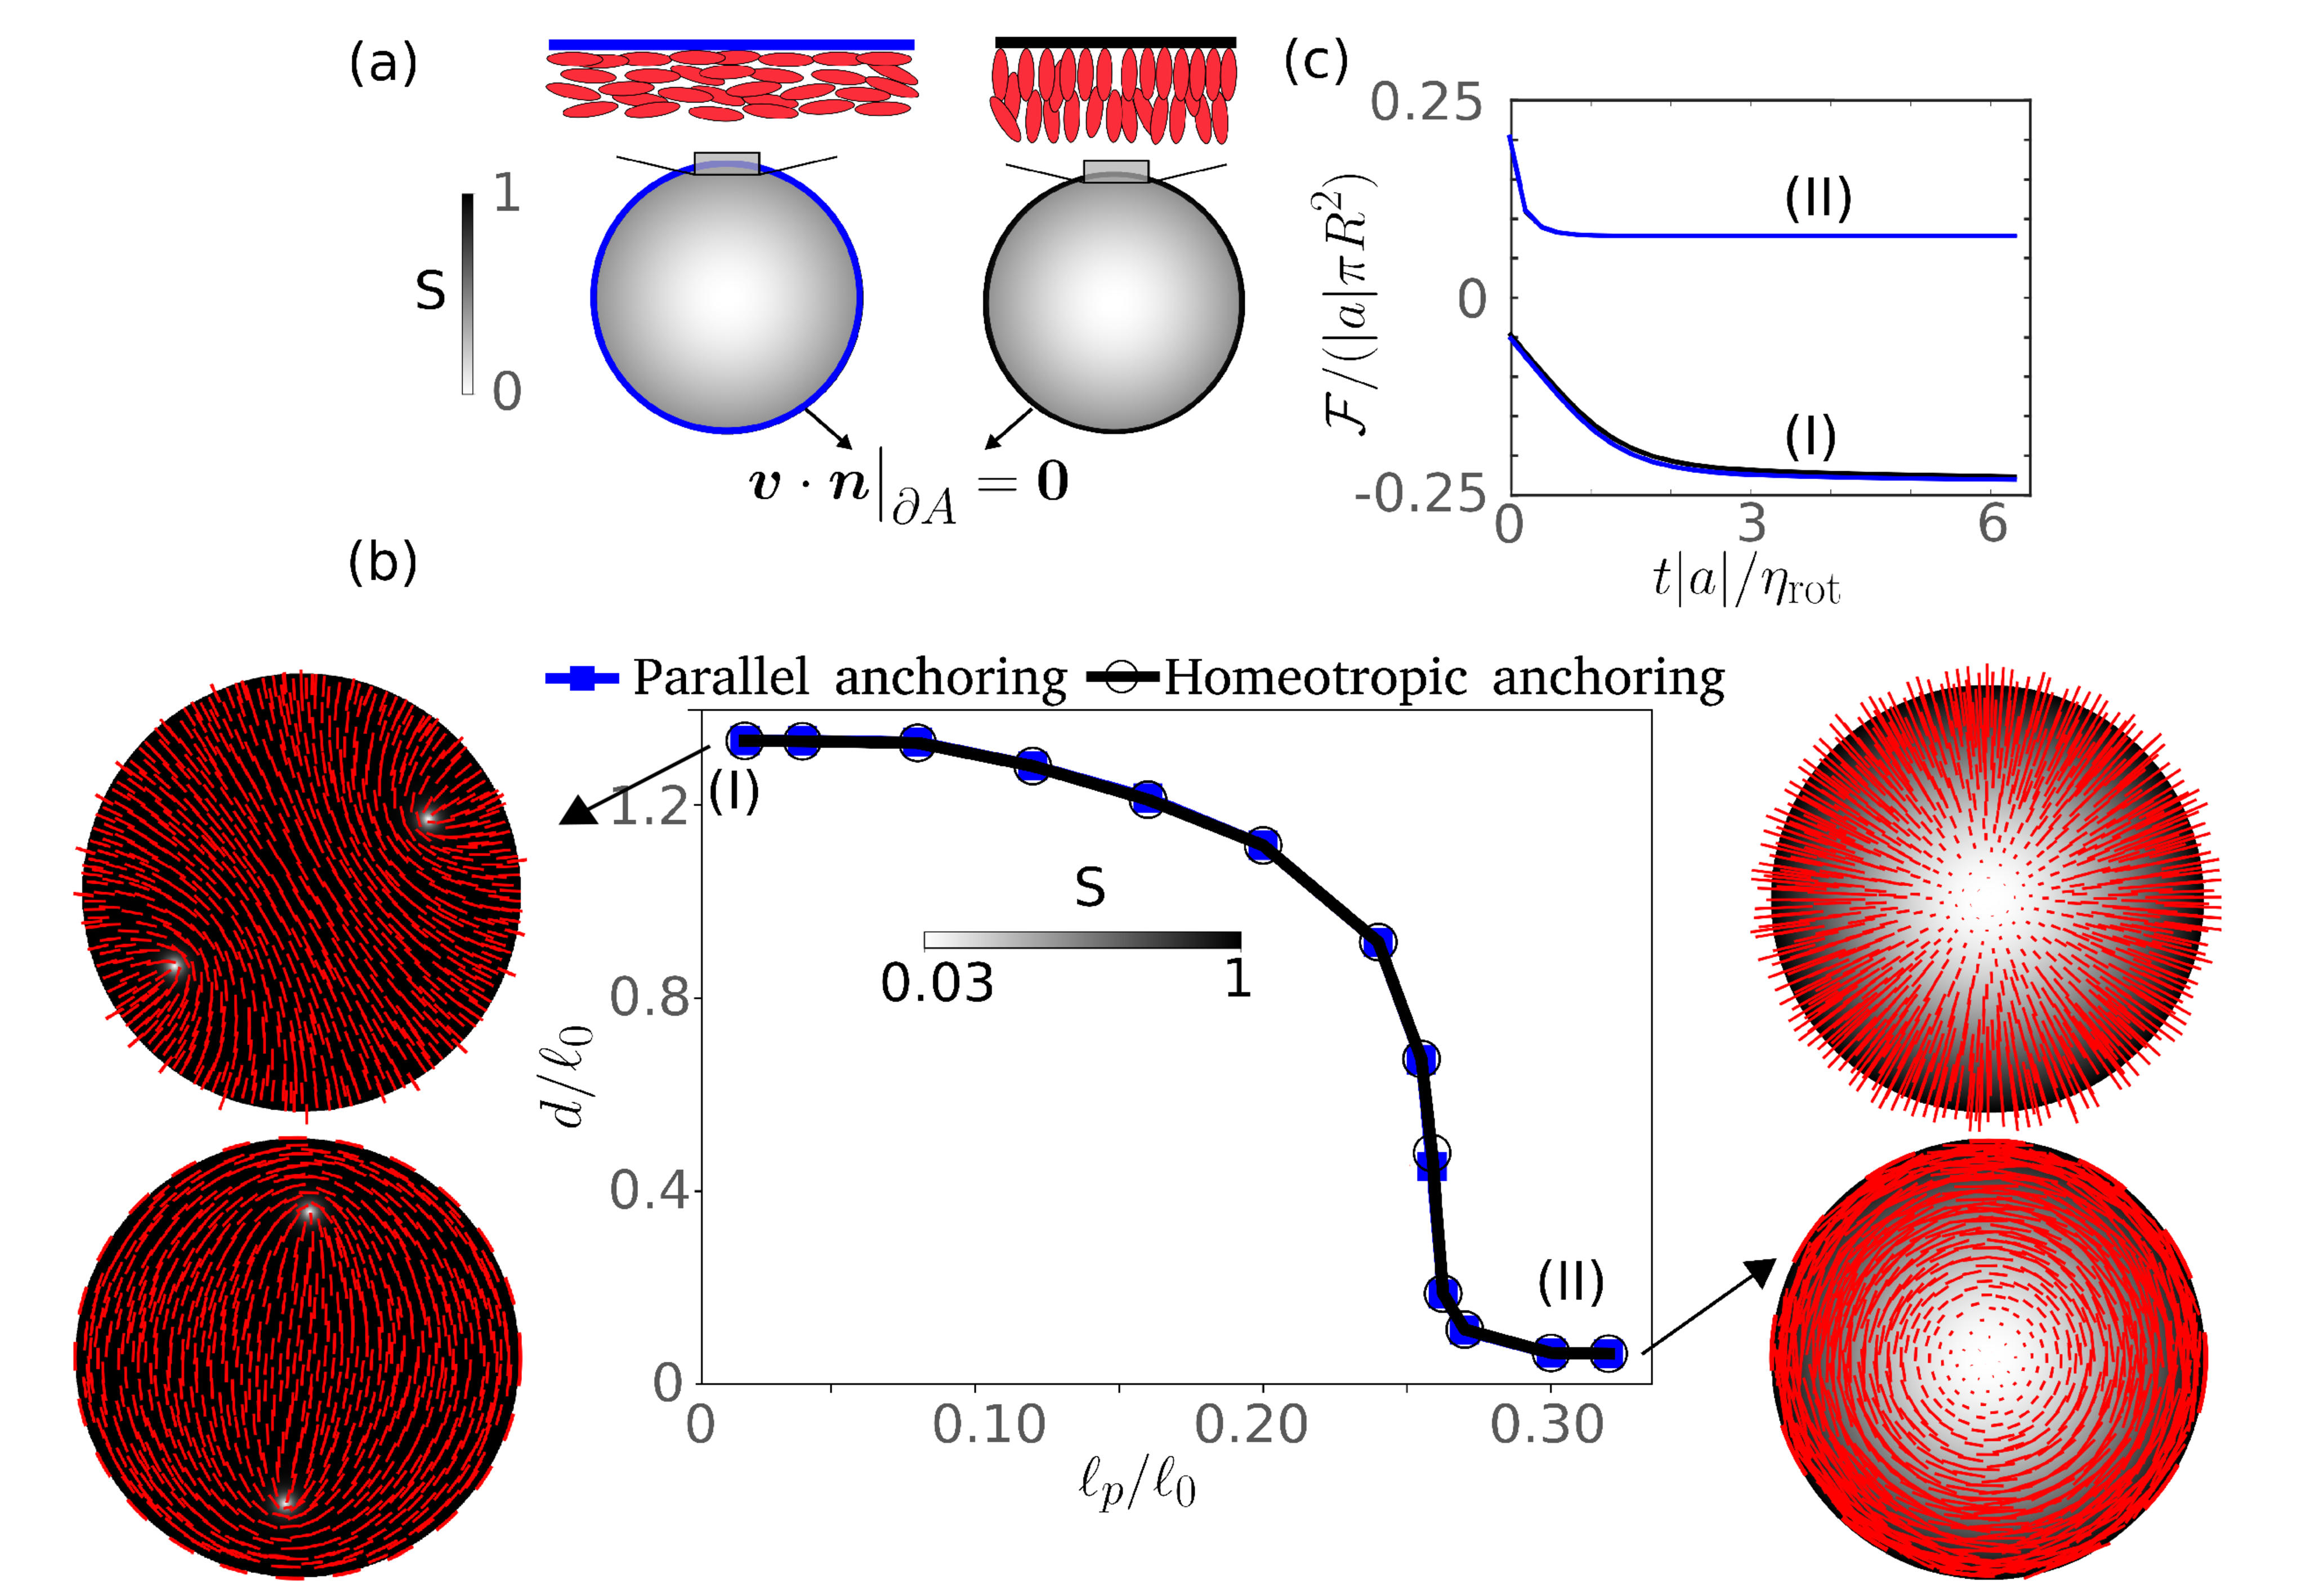
\includegraphics[width=0.85\textwidth]{fig3.eps}
		\caption{\label{sec_1_chap_3_fig_3} \textbf{Effect of nematic correlation length scale $\ell_p$ on the inter-defect distance $d$ in a passive nematic system}. (a) Illustration of nematic and velocity boundary conditions. (b) Inter-defect distance as a function of nematic correlation length scale $\ell_p$ for parallel and homeotropic anchoring conditions, along with selected nematic fields. (c) Monotonically decreasing time-evolution of the Landau free-energy for high and low $\ell_p$ and for both boundary conditions.}
	\end{figure}
	
	We examine next the dynamics of a spatially confined dense contractile active nematic system. In this dense cell colony, density variations are arguably small, and hence the density-dependent aspects of our model may not be important. However, an incompressible model for an active liquid crystal may not be pertinent as convergent/divergent flows are possible due to cell extrusion/proliferation. To simplify the model, we place ourselves in the limit of fast turnover rate, in which density is uniform and convergent/divergent flows are allowed. This only leaves us with the coupling between nematic and velocity fields. In order to model the propensity of cells towards mutual alignment, we set the susceptibility parameter such that the initial nematic order is close to $S_0=\sqrt{-2a/b}=1$. All model parameters are detailed in Table~\ref{modal_parameters_cell_colony}. We impose a boundary condition such that $S=1$ at the boundary and the director field is aligned either tangentially ($\bm{n}$ perpendicular to  $\bm{N}$) or perpendicularly ($\bm{n} = \bm{N}$) to the boundary, corresponding to parallel or homeotropic anchoring, see Fig.~\ref{sec_1_chap_3_fig_3}(a). We enforce that velocity normal to the boundary is zero (impermeable boundary) by introducing a penalty term in the Rayleighian given as  $\int_{\partial A} K \left|\bm{v} \cdot \bm{N}\right|^2 dl$, where $K$ is the penalty coefficient, but allow cells to slide tangentially to the boundary.
	
	We first explore the behavior of a passive nematic system for different ratios between the nematic correlation length  $\ell_p = \sqrt{L/\left(2|a|\right)}$ and the radius of the domain  $\ell_0$.  We start with a spatially correlated random initial condition for $\bm{q}$.  In agreement with previous results, we find that two $+1/2$ defects initially nucleate near the boundary, and then travel away from the wall into the bulk, reaching a quiescent steady-state \cite{hardouin2019,giomi2014}. During this process, the free-energy decreases,  Fig.~\ref{sec_1_chap_3_fig_3}(c), and at steady-state velocities and rate of dissipation vanish. For systems with parallel (homeotropic) boundary conditions, the tips of the $+1/2$ defects point away from (towards) each other, Fig.~\ref{sec_1_chap_3_fig_3}(b). The size of the defect cores relative to system size is controlled by $\ell_p/\ell_0$. As this quantity increases, we expect the two defects to interact and possibly combine into a single $+1$ defect as observed in small-size cell colonies. To examine this, we tracked the distance between the two defects, $d$, as a function of  $\ell_p/\ell_0$, finding that beyond a threshold, $d$ abruptly drops close to zero, with configurations resembling a vortex or an aster depending on boundary conditions, Fig.~\ref{sec_1_chap_3_fig_3}(b). We note, however, that in the absence of activity, $d$ stays finite, and hence the two defects do not strictly become a $+1$ defect, which can be understood in terms of a Coulomb-like repulsion \cite{thijssen2020, vafa2020}.
	
	
	We next explore the spatiotemporal behavior of defects in a contractile ($\lambda_{\rm aniso} > 0$) active nematic system by examining the  velocity and nematic fields as a function activity, measured by the active length scale $\ell_a = \sqrt{L/\lambda_{ \rm aniso}}$. We vary this inverse activity parameter at low nematic correlation length scale $\ell_p/\ell_0 = 0.02$ and focus on parallel boundary conditions for the nematic field, see Fig.~\ref{sec_1_chap_3_fig_3.5}.  At low activity (large $\ell_a/\ell_0$), we observe that the active contractile stress $\lambda_{\rm aniso} \bm{q}$ leads to new steady-state with a smaller inter-defect distance, Fig.~\ref{sec_1_chap_3_fig_3.5}(b) and left panel of Movie~2. More importantly, the steady state of the active system exhibits persistent flows in the nose to tail direction around defects \cite{doostmohammadi2018,ronning2022}, which push these defects by advection of nematic order, Eq.~(\ref{jaumann_detivative_def}). The passive nematic distribution is also distorted  by the flow-induced alignment term involving $\beta$.
	
	\begin{figure}[tb]
		\centering
		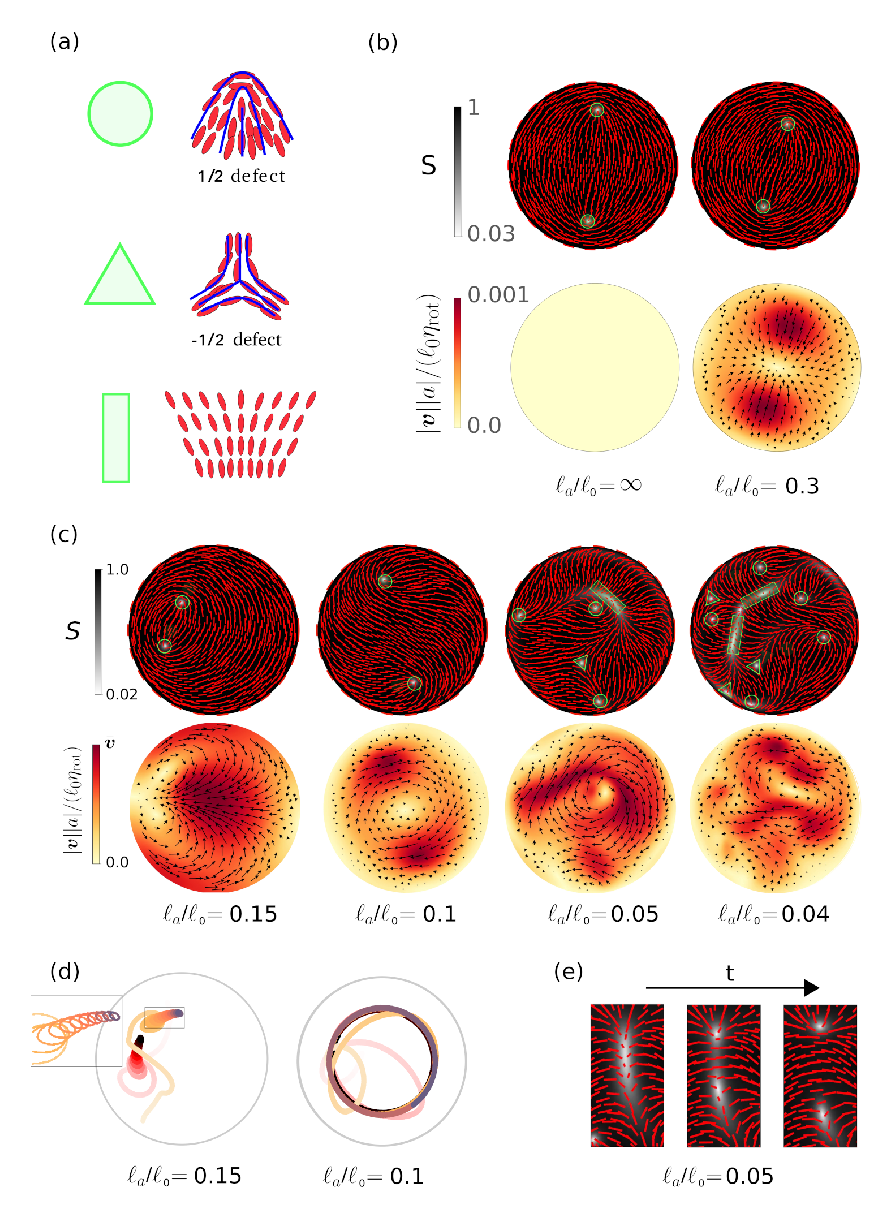
\includegraphics[width=0.77\textwidth]{fig4.eps}
		\caption{\label{sec_1_chap_3_fig_3.5}  \textbf{Effect of activity on a dense confined colony of contractile cells.} (a) Graphical coding of $\pm \frac{1}{2}$ defects and of splay bands. (b) Nematic field (top, with segment showing nematic direction and colormap showing order parameter $S$) and velocity field (bottom) in absence (left) and presence (right) of activity.	(c) Effect of activity on the system dynamics. The velocity scale $\bar{\bm{v}}$ is varied to ease visualization ($\bar{\bm{v}} = 0.14, 0.16, 0.19, 0.3$ from left to right). (d) Dynamics of the two $+1/2$ defects for $\ell_a/\ell_0=0.15$ and $\ell_a/\ell_0=0.1$. Defect trajectories become darker as time increases. (e) Nucleation of $1/2$ and  $-1/2$ defects from splay bands at $\ell_a/\ell_0=0.05$. See Movie 2 for $\ell_a/\ell_0=0.3$ to 0.1 and Movie 3 for $\ell_a/\ell_0=0.05$ and 0.04. }
	\end{figure}
	
	
	At a smaller value, $\ell_a/\ell_0 = 0.15$, the two motile $+1/2$ defects move closer together and  towards the wall, with an out-of-equilibrium velocity exhibiting two vortices. After a transient wiggling motion, these to defects stop moving and the system reaches an out-of-equilibrium steady-state,  Fig.~\ref{sec_1_chap_3_fig_3.5}c,d and center panel of Movie~2. As we further reduce the ratio $\ell_a/\ell_0$ to $0.1$, the defect distance increases and the two defects rotate in a chiral configuration leading to persistent rotation of the entire system, Fig.~\ref{sec_1_chap_3_fig_3.5}c,d and 
	right panel of Movie~2. It has been suggested  that the length-scale of such vortex driven by a defect pair is commensurate to $\ell_a$ \cite{chandrakar2020}, and therefore, for lower activity this length-scale is too large for vortices to develop within the domain size. %In this regime, the spiral flow suppresses the defect nucleation that might otherwise form through the splay-type hydrodynamic instability \cite{ramaswamy2007, ramaswamy2010}. A similar argument has been made here for bend-type instability for an extensile network of microtubules and  kinesins \cite{opathalage2019}. 
	Upon further lowering the active length scale, $\ell_a/\ell_0 \leq 0.05$, we observe the formation of splay bands, which destabilize into point defects as previously described \cite{ramaswamy2007, ramaswamy2010}, Fig.~\ref{sec_1_chap_3_fig_3.5}d (right) and Movie 3. In this regime, active stresses overcome the restoring elastic stresses and distort the nematic field to form lines of splay-type disinclination in the bulk and close to the boundary. These disclination lines destabilize and split into pairs of $\pm 1/2$ defects, Fig.~\ref{sec_1_chap_3_fig_3.5}e, which move and annihilate with defects of opposite charge. The persistent generation of disclination lines, their destabilization into point defects, and the motion and annihilation of these defects gives rise to active turbulence. At any given time, the system exhibits more than two defects but the total topological charge is conserved to $+1$.
	
	In summary, in a confined passive nematic system, our simulations recover the canonical spontaneous organization of two $+1/2$ defects with a steady inter-defect distance decreasing with increasing  passive nematic length scale $\ell_p  = \sqrt{L/\left(2|a| \right)}$. In an active system, our simulations exhibit a diversity of dynamical regimes depending on the active nematic length-scale $\ell_a= \sqrt{L/\lambda_{\rm aniso}}$. Because a gradient in nematic order in the vicinity of defects generates an active flow, defects become motile. At large or intermediate values of $\ell_a/\ell_0$, defects pairs move closer together, break symmetry and wobble closer to the boundary, or develop a persistent spiral motion. At small values of  $\ell_a/\ell_0$ (high activity), we observe active turbulence characterized by persistent defect nucleation due to splay-type instabilities, motion and annihilation. 
	
	\section{Summary and outlook} \label{summary}
	
	We have proposed a general modeling framework for density-dependent active nematic systems in 2D. This framework relies on Onsager's variational principle for irreversible thermodynamics. We have reviewed the history of this variational approach and discussed how it naturally provides a simple and direct  procedure to develop thermodynamically consistent models in fully nonlinear regimes. Focusing on density-dependent active nematic fluids, we have shown that this formalism enables a clear and systematic derivation of otherwise complex governing equations coupling nematic order, gel velocity and density. Neglecting density variations, we have recovered using our variational approach a standard model for incompressible active nematics. We have then particularized the general framework to develop a specific density-dependent active nematic fluid gel. We have developed a numerical finite element method to approximate this model and applied it to two studies of biological relevance. In the first study, we have explored the role of the self-organization of the actin cytoskeleton during wound repair. In our simulations, a slight overactivity around the wound drives a self-reinforcing flow of the actin gel, leading to the self-organization of a nematic bundle that efficiently constricts the wound. In this example, nematic oder arises due to activity, as self-reinforcing flows locally densify and orient nematic order. This mechanism of active pattern formation of dense nematic structures is further studied in \cite{mirza2022} to understand the physical basis of self-organization of the actin cytoskeleton. In a second numerical study, we explore the self-organization of a dense nematic system in the limit of high turnover, modeling a constrained colony of contractile elongated cells. Here, the ordering mechanisms is crowding. Depending on the magnitude of the activity, the topological defects required by boundary conditions either reach a steady state or exhibit highly dynamical flows as well as active turbulence. If suitably extended to curved and time-evolving surface domains \cite{mirza2023}, the framework presented here can help elucidate the interaction between nematodynamics and reshaping during morphogenesis from cellular to organism scales \cite{mayer2010,maroudas2021}.
	
	
	
	%compressible active nematic model to study the self-organization of actin networks into versatile architectures. We first propose a systematic derivation of a compressible active nematic model based on   Onsager's variational framework. The derivation starts with generalized potential functionals that model the elastic, dissipative, out-of-equilibrium behavior and physical constraints of the active nematic gel. Using the potential functional, a constrained-optimization problem is solved by minimizing the potential functionals with respect to process variables and maximizing with respect to the physical constraints to obtain the generic governing equations of the model. An additional constraint on the density field is introduced by the mass conservation equation. The governing equations are then particularized to the actin cytoskeleton by formulating elastic free energy functional that governs the anisotropy of architecture based on Landau expansion of free energy, a quadratic dissipation potential that governs the irreversible dynamics and power functional that models the contractile forces exerted by the bundling proteins in both isotropic and anisotropic networks. The turnover dynamics of the cytoskeleton is introduced as a constraint in the mass conservation equation. Next, we propose a systematic numerical solution of the proposed compressible active nematic model. The numerical solution is based on the variational formulation of Onsager formalism in which the functionals are discretization in space using the finite element method and time discretization using the implicit Euler scheme. The discrete functionals are then minimized using discrete process variables to obtain the weak form of the governing equations. Finally, we explore the numerical solution of the model in two studies of biological relevance. In the first study, we explore the role of actin cytoskeleton architecture in wound repair. We show that a slight overactivity of bundling proteins around the wound drives a self-reinforcing flow of the actin network leading to self-organization of the nematic bundle that serves to constrict the wound. In the second numerical study, we explore the self-organization of nematic architectures in the limit of high turnover in a constrained colony of contractile cells. The cell colony exhibits a density-dependent isotropic-to-nematic transition, self-organizing two $+1/2$ integer defects. Depending on the magnitude of contractility, the topological defects either reach the study state or exhibit highly dynamical vortical flows as well as active turbulence.
	
	%Our framework provides a basis to explore a large variety of active systems that involve the self-organization of architectures where a tight coupling between nematics, hydrodynamics, and density plays an essential role. Although here we have focused on simple cases where the nematic architectures are self-organized in a contractile network due to slight overactivity of myosin in the cytoskeleton or due to boundary conditions in a colony of contractile cells, our framework can be applied to understand the diversity of nematic architectures in actomyosin networks \cite{mirza2022}, including bundles  \cite{tojkander2015,jalal2019, vignaud2021}, asters \cite{xia2019}, and tactoids \cite{weirich2017,weirich2019}. If suitably extended to curved and time-evolving surface domains \cite{mirza2023}, the framework presented here can help us examine the interaction between nematodynamics and reshaping during cytokinesis \cite{mayer2010} or hydra morphogenesis \cite{maroudas2021}.
	
	%Furthermore, it will be interesting to consider viscoelasticity as there is evidence indicating the transition of viscous actin bundles into stress-bearing viscoelastic bundles as the pattern matures due to remodeling with the substrate \cite{gupta2015} or due to localization of crosslinkers \cite{Banerjee2020}. Furthermore, the minimal model of a
	%single field representing actin bundling species chosen here could be extended to several species and interactions between them. These extended models could represent, for example, the coexistence of diverse actin architectures such as asters and nematic bundles, with each protein responsible for an individual actin architecture.
	
	
	\section*{Acknowledgments}
	The authors acknowledge the support of the European Research Council (CoG-681434) and the Spanish Ministry for Science and Innovation (PID2019-110949GB-I00). WM acknowledges the La Caixa Fellowship  and the European Union’s Horizon 2020 research and innovation program under the Marie Skłodowska-Curie action (GA 713637). MA acknowledges the Generalitat de Catalunya (ICREA Academia prize for excellence in research). IBEC and CIMNE are recipients of a Severo Ochoa Award of Excellence.
	
	\appendix
	%\section{Rate of change of a frame-indifferent free energy density}\label{app:rate_of_change_energy}
	
	%\mab{[I rewrote this appendix without the need to define artificially the Jaumann derivative of  $\nabla \bm{q}$. Please check it.]}
	
	
	%We derive next an expression for the material time derivative of the free energy density, $\dot{f}$. With this aim, we perform first required preliminary calculations. 
	
	%Partial time-differentiation commutes with partial space differentiation. However, the material time-derivative and $\nabla$ do not commute, and for this reason we introduce a more explicit notation for the material time-derivative as $D/Dt$ when required for clarity. %Likewise, when required, we write the Jaumann derivative by $\delta/\delta t$. 
	%The material time derivative of $\nabla \bm{q}$ is given by
	%\begin{equation}
	%\frac{D}{Dt} \left(\nabla_c q_{ab}\right) = \partial_t  \nabla_c q_{ab} + v_d  \nabla_d \nabla_c q_{ab},
	%\end{equation}
	%whereas the gradient of the material time derivative of $\bm{q}$ is
	%\begin{eqnarray}
	% \nabla_c \dot{q}_{ab} & = \nabla_c \left(\frac{D}{Dt} {q}_{ab}\right) = \nabla_c \partial_t   q_{ab} + \nabla_c v_d \nabla_d q_{ab} + v_d  \nabla_c \nabla_d  q_{ab} \nonumber \\ & = \frac{D}{Dt} \left(\nabla_c q_{ab}\right) + \nabla_c v_d q_{ab} \nonumber \\ & = \frac{D}{Dt} \left(\nabla_c q_{ab}\right) + d_{dc} \nabla_d q_{ab} + w_{dc} \nabla_d q_{ab}.\label{aux1}
	%\end{eqnarray}
	%From the definition of Jaumann derivative, we can compute its gradient as
	%\begin{eqnarray}
	%\nabla_c \widehat{q}_{ab} =  \nabla_c \dot{q}_{ab}  + \nabla_c q_{ad} w_{db} + q_{ad}\nabla_c  w_{db}  + \nabla_c q_{db} w_{da} + q_{db} \nabla_c  w_{da}.
	%\end{eqnarray}
	%Using Eq.~(\ref{aux1}) and the definition in Eq.~(\ref{zeta}), we can rewrite this expression as 
	%\begin{eqnarray}
	%\nabla_c \widehat{q}_{ab} = &  \frac{D}{Dt} \left(\nabla_c q_{ab}\right) + d_{dc} \nabla_d q_{ab} + w_{dc} \nabla_d q_{ab}  +  w_{db} \nabla_c q_{ad} + w_{da} \nabla_c q_{db}  \nonumber \\ & +  \left(q_{ad}\epsilon_{db}   - \epsilon_{ad} q_{db} \right)\zeta_c.
	%\end{eqnarray}
	%From this expression and the chain rule, the rate of change of $f$ can be written as
	%  \begin{eqnarray} 
		%	\dot{f} &= &  \frac{\partial f}{\partial q_{ab}} \dot{q}_{ab}+ \frac{\partial f}{\partial \nabla_c q_{ab}} \frac{D}{Dt} \left(\nabla_c q_{ab}\right)  \nonumber\\
		%	&= & \frac{\partial f}{\partial q_{ab}} \left(\widehat{q}_{ab}- q_{ad} w_{db}- q_{db} w_{da}\right)   + \frac{\partial f}{\partial \nabla_c q_{ab}} \bigg[ \nabla_c \widehat{q}_{ab} +  2\epsilon_{ad} q_{db}   \zeta_c \nonumber\\ && \;\;\;\;\; - d_{dc} \nabla_d q_{ab}  - w_{dc} \nabla_d q_{ab}  -  w_{db} \nabla_c q_{ad} - w_{da} \nabla_c q_{db}  \bigg], \label{eq:dotfUUUU}  
		%\end{eqnarray}
		%where we have used the symmetry of $\bm{q}$ and the antisymmetry of $\bm{\epsilon}$ to simplify the term involving $\zeta_c$.
		
		%The free energy density $f$ should be frame indifferent, and hence its material time derivative should vanish, $\dot{f}=0$, for any rigid body motion characterized by  $d_{ab}=0$, $\widehat{q}_{ab}=0$, and uniform but otherwise arbitrary $w_{ab}$, and hence $\zeta_c = 0$. Particularizing Eq.~(\ref{eq:dotfUUUU}) to a rigid body motion, we find that 
		%\begin{eqnarray} 
		%	0 &= & \frac{\partial f}{\partial q_{ab}} \left(  q_{ad} w_{db}+ q_{db} w_{da}\right) \nonumber \\
		%	&&  + \frac{\partial f}{\partial \nabla_c q_{ab}} \bigg[   w_{dc} \nabla_d q_{ab}  +  w_{db} \nabla_c q_{ad} + w_{da} \nabla_c q_{db}  \bigg],
		%\label{f_frame_indiff}
		%\end{eqnarray}
		%for all antisymmetric tensors $\bm{w}$ and for all fields $\bm{q}$. Further particularizing this equation to uniform nematic fields ($\nabla\bm{q} = \bm{0}$)  and spin tensors of the form $\bm{w} = \bm{\epsilon}$, we obtain the condition 
		%\begin{equation} 
		%	0 =  \frac{\partial f}{\partial q_{ac}} q_{cb} - \frac{\partial f}{\partial q_{bc}} q_{ca}.
		%\label{f_frame_indiff_2}
		%\end{equation}
		%Similarly, considering a point where the nematic field is zero but its gradient is not, we obtain
		%\begin{equation} 
		%	0 =  \frac{\partial f}{\partial \nabla_a q_{cd}} \nabla_b q_{cd} -  \frac{\partial f}{\partial \nabla_b q_{cd}} \nabla_a q_{cd} + 	
		%	 2\left(\frac{\partial f}{\partial \nabla_d q_{ac}} \nabla_d q_{cb} - \frac{\partial f}{\partial \nabla_d q_{bc}} \nabla_d  q_{ca}\right).
		%\label{f_frame_indiff_3}
		%\end{equation}
		
		
		%Combining Eqs.~(\ref{f_frame_indiff}) and (\ref{eq:dotfUUUU}), we finally obtain Eq.~\eqref{eq:final_rate_of_free_energy}. A more direct and elegant geometric derivation of this result follows from writing down the free energy in a general curvilinear coordinate system and expressing the Jaumann derivative in terms of Lie derivatives \cite{mirza2023,waleed_thesis}.
		%  \begin{eqnarray} 
			%	\dot{f} &= &  \frac{\partial f}{\partial q_{ab}} \widehat{q}_{ab}   + \frac{\partial f}{\partial \nabla_c q_{ab}} \left[ \nabla_c \widehat{q}_{ab} +  \left(\epsilon_{ad} q_{db}    - q_{ad}\epsilon_{db}\right)\zeta_c  - d_{dc} \nabla_d q_{ab}  \right]. 
			%\end{eqnarray}
			
			
			\section{Conditions for non-negative entropy production} \label{inequality}
			
			We identify here the conditions for non-negative entropy production. It is obvious that $\mathcal{D}\left[\bm{0},\bm{0}\right]=0$. We thus examine when $\mathcal{D}$ is non-negative and convex. The integrand $d$ can be written as 
			\begin{eqnarray}
				d(\bm{v},\bm{d},\widehat{\bm{q}}) &  = \eta \big( d_{ab} d_{ab}   + (\text{tr}d)^2  \big) + \frac{\eta_{\text{rot}}}{2} \widehat{q}_{ab} \widehat{q}_{ab}  + \beta d_{ab}^{\rm dev}\widehat{q}_{ab} + \frac{\gamma}{2} v_a v_a \geq 0  \nonumber\\ 
				& = 2\eta \big( d_{11}^2 + d_{12}^2 + d_{22}^2  + d_{11}d_{22} \big) + \eta_{\text{rot}} \big( \widehat{q}_{1}^{\, \, 2} + \widehat{q}_{2}^{\, \, 2}  \big)  \\ 
				&  + \beta \big(d_{11}\widehat{q}_{1} - d_{22}\widehat{q}_{1} + \nonumber  2d_{12}\widehat{q}_{2}\big) +  \nonumber  \frac{\gamma}{2} \big(v_1^{\,2} + v_2^{\,2}\big) \geq 0 .
			\end{eqnarray}
			and hence it is a quadratic form of its arguments that can be expressed as $d = z_{a} M_{ab} z_b$ with 
			\begin{equation}
				\bm{z} = \left(\begin{array}{c}
					d_{11}\\ 
					d_{22}\\ 
					d_{12}\\ 
					q_{1}\\ 
					q_{2}\\ 
					v_1\\ 
					v_2\\ 
				\end{array}\right), \quad  \bm{M} = \left(\begin{array}{ccccccc}
					2\eta& \eta &0  &\beta/2  &0  &0  &0   \\ 
					\eta& 2\eta &0  &-\beta/2  &0  &0  &0   \\ 
					0&  0&  2\eta&  0& \beta &0  &0   \\ 
					\beta/2& -\beta/2 &0  &\eta_{\rm rot}  &0  &0  &0   \\ 
					0&  0 &\beta  & 0 & \eta_{\rm rot} &0  &0   \\ 
					0& 0 & 0 & 0 & 0 & \gamma/2 & 0  \\ 
					0& 0 & 0 & 0 & 0 & 0 & \gamma/2
				\end{array}\right).
			\end{equation}
			Because $\bm{z}$ is a linear function of $\left(\bm{v},\widehat{\bm{q}}\right)$, a direct argument shows that if the symmetric matrix $\bm{M}$ is positive semi-definite, then $\mathcal{D}\left[\bm{v},\widehat{\bm{q}}\right]$ is a non-negative and convex functional. According to Sylvester's criterion \cite{doi:10.1080/00029890.1991.11995702}, $\bm{M}$ is positive semi-definite if and only if its leading principal minors are non-negative. As simple calculation shows that, since $\eta>0$, $\eta_{\rm rot}>0$ and $\gamma>0$, this condition is met when
			\begin{equation}
				2\eta \eta_{\rm rot} - \beta^2 \geq 0.
			\end{equation}
			
			
			
			
			\section{Equivalence between different forms of balance of linear momentum} \label{equivalence}
			
In this section,  establish an equivalence between the governing equations for balance of linear momentum obtained in Sections \ref{sec_2} and \ref{sec_4}. Comparing Eqs.~(\ref{eq:weak_v}) and (\ref{eq:weak_v_disc}), we need to prove that 
						\begin{eqnarray}
				C_1 = &\int_A \left\{-\frac{ f}{\rho} \nabla_d \left(\rho u_d\right) + \frac{\epsilon_{ab}}{2} \frac{\partial ( d+ p)}{\partial {\zeta}_c} \nabla_c \nabla_b {u}_a  \right. \nonumber \\ & \left. + \frac{\partial ( d+ p)}{\partial \widehat{q}_{ab}}  \left[ {u}_c\nabla_c{q}_{ab} + \frac{1}{2}\left({q}_{ac} {\epsilon}_{cb} -{\epsilon}_{ac}{q}_{cb} \right) {\epsilon}_{ef}\nabla_f{u}_e\right] \right\}\rho dA \nonumber\\
				&+  \int_{\partial A} f\rho N_c u_c dl - \int_{\partial_{N_{\bm{L}}} A} L_{ab} \left[ {u}_c\nabla_c{q}_{ab} + \frac{1}{2}\left({q}_{ac} {\epsilon}_{cb} -{\epsilon}_{ac}{q}_{cb} \right) {\epsilon}_{ef}\nabla_f{u}_e\right]dl \nonumber\\& -\int_{\partial_{N_{\bm{\Gamma}}} A} \Gamma_{ab} \nabla_b u_a dl , \label{eq:weak_v_disc_app}
\end{eqnarray}
 is equal to 
\begin{equation}
				C_2 = \int_A \bar{\sigma}_{ab}\nabla_b u_a dA, \label{eq:weak_v_app}
			\end{equation}
where $\bar{\sigma}_{ab}$ is the total stress except for the terms involving $\partial(d+p)/\partial\bm{d}$ and $\partial(d+p)/\partial\bm{w}$, and it is given by
\begin{eqnarray}
				\bar{\sigma}_{ab} = & -\rho\frac{\partial  f}{\partial \nabla_b q_{dc}} \nabla_a q_{dc}  +   q_{ad}  \nabla_c \left(\rho \frac{\partial f}{\partial \nabla_c {q}_{bd}}\right) - q_{bd}\nabla_c \left(\rho \frac{\partial f}{\partial \nabla_c {q}_{ad}}\right) \nonumber \\ &  -  \frac{1}{2} \nabla_c \left(\rho\frac{\partial (  d+p)}{\partial \zeta_c} \right) \epsilon_{ab}   .
	\end{eqnarray}


Integrating by parts the first term, and accounting for balance of generalized force in Eq.~\eqref{eq:balance_q} to substitute $\partial(d+p)/\partial\widehat{\bm{q}}$, we have 
\begin{eqnarray}
C_1 = &\int_A \left\{ u_d \nabla_d f + \frac{\epsilon_{ab}}{2} \frac{\partial ( d+ p)}{\partial {\zeta}_c} \nabla_c \nabla_b {u}_a  \right. \nonumber \\ & \left. + \left[\frac{1}{\rho}\nabla_d \left(\rho \frac{\partial f}{\partial \nabla_d q_{ab}} \right) - \frac{\partial f}{\partial q_{ab}}\right] \left[ {u}_c\nabla_c{q}_{ab} + \frac{1}{2}\left({q}_{ac} {\epsilon}_{cb} -{\epsilon}_{ac}{q}_{cb} \right) {\epsilon}_{ef}\nabla_f{u}_e\right] \right\}\rho dA \nonumber\\
&- \int_{\partial_{N_{\bm{L}}} A} L_{ab} \left[ {u}_c\nabla_c{q}_{ab} + \frac{1}{2}\left({q}_{ac} {\epsilon}_{cb} -{\epsilon}_{ac}{q}_{cb} \right) {\epsilon}_{ef}\nabla_f{u}_e\right]dl \nonumber\\& -\int_{\partial_{N_{\bm{\Gamma}}} A} \Gamma_{ab} \nabla_b u_a dl.
\end{eqnarray}
Integrating by parts the first term within square brackets in the second line of this equation, we obtain
\begin{eqnarray}
C_1 = &\int_A \left\{ u_d \nabla_d f + \frac{\epsilon_{ab}}{2} \frac{\partial ( d+ p)}{\partial {\zeta}_c} \nabla_c \nabla_b {u}_a  \right. \nonumber \\  
& -  \frac{\partial f}{\partial \nabla_d q_{ab}} \nabla_d\left[ {u}_c\nabla_c{q}_{ab} + \frac{1}{2}\left({q}_{ac} {\epsilon}_{cb} -{\epsilon}_{ac}{q}_{cb} \right) {\epsilon}_{ef}\nabla_f{u}_e\right]  \nonumber\\
&\left.  - \frac{\partial f}{\partial q_{ab}} \left[ {u}_c\nabla_c{q}_{ab} + \frac{1}{2}\left({q}_{ac} {\epsilon}_{cb} -{\epsilon}_{ac}{q}_{cb} \right) {\epsilon}_{ef}\nabla_f{u}_e\right] \right\}\rho dA \nonumber\\
&- \int_{\partial_{N_{\bm{L}}} A}\left( L_{ab} - \rho \frac{\partial f}{\partial \nabla_d q_{ab}} N_d \right)\left[ {u}_c\nabla_c{q}_{ab} + \frac{1}{2}\left({q}_{ac} {\epsilon}_{cb} -{\epsilon}_{ac}{q}_{cb} \right) {\epsilon}_{ef}\nabla_f{u}_e\right]dl \nonumber\\& -\int_{\partial_{N_{\bm{\Gamma}}} A} \Gamma_{ab} \nabla_b u_a dl.
\end{eqnarray}
The boundary integral over $\partial_{N_{\bm{L}}} A$ vanishes because of the boundary condition in Eq.~\eqref{eq:balance_q_bd}. Noting that 
\begin{equation}
\nabla_d f = \frac{\partial f}{\partial q_{ab}}\nabla_d q_{ab} + \frac{\partial f}{\partial \nabla_c q_{ab}} \nabla_c \nabla_d q_{ab}, 
\end{equation}
we can cancel three terms in the first three lines of this equation to obtain
\begin{eqnarray}
C_1 = &\int_A \left\{ \frac{\epsilon_{ab}}{2} \frac{\partial ( d+ p)}{\partial {\zeta}_c} \nabla_c \nabla_b {u}_a  \right. \nonumber \\  
& -  \frac{\partial f}{\partial \nabla_d q_{ab}} \nabla_d\left[  \frac{1}{2}\left({q}_{ac} {\epsilon}_{cb} -{\epsilon}_{ac}{q}_{cb} \right) {\epsilon}_{ef}\nabla_f{u}_e\right]  -  \frac{\partial f}{\partial \nabla_d q_{ab}} \nabla_d {u}_c\nabla_c{q}_{ab} \nonumber\\
&\left.  - \frac{\partial f}{\partial q_{ab}} \left[  \frac{1}{2}\left({q}_{ac} {\epsilon}_{cb} -{\epsilon}_{ac}{q}_{cb} \right) {\epsilon}_{ef}\nabla_f{u}_e\right] \right\}\rho dA \nonumber\\
\nonumber\\& -\int_{\partial_{N_{\bm{\Gamma}}} A} \Gamma_{ab} \nabla_b u_a dl.
\end{eqnarray}
Because of frame indifference of $f$ as expressed by Eq.~(\ref{f_frame_indiff_2}), the term in the third line vanishes. Furthermore, using the symmetry of $\bm{q}$, we can simplify the second line as
\begin{eqnarray}
C_1 = &\int_A \left\{ \frac{\epsilon_{ab}}{2} \frac{\partial ( d+ p)}{\partial {\zeta}_c} \nabla_c \nabla_b {u}_a  \right. \nonumber \\  
&\left.  -  \frac{\partial f}{\partial \nabla_d q_{ab}} \nabla_d \left(  {q}_{ae} \nabla_b {u}_e -  {q}_{ae} \nabla_e {u}_b\right)  -  \frac{\partial f}{\partial \nabla_d q_{ab}} \nabla_d {u}_c\nabla_c{q}_{ab} \right\}\rho dA \nonumber\\
\nonumber\\& -\int_{\partial_{N_{\bm{\Gamma}}} A} \Gamma_{ab} \nabla_b u_a dl.
\end{eqnarray}
 Then, integration by parts of the term in the first line and the first term in the second line yields
\begin{eqnarray}
C_1 = &\int_A \left\{-\frac{1}{2}\nabla_c\left(\rho  \frac{\partial ( d+ p)}{\partial {\zeta}_c}\right) \epsilon_{ab} \nabla_b {u}_a  \right. \nonumber \\  
& \left. +   \nabla_d\left( \rho\frac{\partial f}{\partial \nabla_d q_{ab}}\right) \left(  {q}_{ae} \nabla_b {u}_e -  {q}_{ae} \nabla_e {u}_b\right)  -  \rho\frac{\partial f}{\partial \nabla_d q_{ab}} \nabla_d {u}_c\nabla_c{q}_{ab} \right\} dA \nonumber\\
& -\int_{\partial_{N_{\bm{\Gamma}}} A} \left( \Gamma_{ab} -  \frac{1}{2} \rho  \frac{\partial ( d+ p)}{\partial {\zeta}_c} N_c \epsilon_{ab} \right)\nabla_b u_a dl \nonumber \\
& -\int_{\partial_{N_{\bm{\Gamma}}} A}   \rho\frac{\partial f}{\partial \nabla_d q_{ab}} N_d \left(  {q}_{ae} \nabla_b {u}_e -  {q}_{ae} \nabla_e {u}_b\right)  dl.
\end{eqnarray}
Renaming the dummy indices conveniently, we obtain
\begin{eqnarray}
C_1 = &\int_A \left\{-\frac{1}{2}\nabla_c\left(\rho  \frac{\partial ( d+ p)}{\partial {\zeta}_c}\right) \epsilon_{ab}  \right. \nonumber \\  
& \left. +  {q}_{ae} \nabla_d\left( \rho\frac{\partial f}{\partial \nabla_d q_{eb}}\right)   -    {q}_{be}\nabla_d\left( \rho\frac{\partial f}{\partial \nabla_d q_{ea}}\right)    -  \rho\frac{\partial f}{\partial \nabla_b q_{ef}} \nabla_a{q}_{ef} \right\} \nabla_b {u}_a  dA \nonumber\\
& -\int_{\partial_{N_{\bm{\Gamma}}} A} \left\{ \Gamma_{ab} -  \left[\frac{1}{2} \rho  \frac{\partial ( d+ p)}{\partial {\zeta}_c} \epsilon_{ab} - {q}_{ae} \left( \rho\frac{\partial f}{\partial \nabla_c q_{eb}}\right)   +   {q}_{be}\left( \rho\frac{\partial f}{\partial \nabla_c q_{ea}}\right) \right] N_c \right\}\nabla_b u_a dl.\nonumber
\end{eqnarray}
Recalling the boundary condition in Eq.~(\ref{eq:balance_angular_momentum}), the boundary term vanishes. Finally, a direct comparison of the bulk term with Eq.~(\ref{eq:weak_v_app}) shows that $C_1 = C_2$.

			
			\section{Numerical convergence} \label{appendix_grid}
			
			
			We verify our numerical methods for the spatial discretization by solving the proposed model for various mesh sizes. For this purpose, we consider a passive nematic system with circular confinement, see Fig.~\ref{sec_1_chap_3_fig_3}, and $\ell_p/\ell_0=0.04$. We define the normalized error of free-energy at steady state
			\begin{equation}	
				E_x = \frac{|F^h -F^*|}{|F^*|} , 
			\end{equation}
			where $F^h$ is the free-energy of a finite element solution with mesh-size $h$ and $F^*$ is that of an overkill solution computed with a very fine mesh of $n_e = 695,296$ triangular elements. We plot the energy error for decreasing mesh sizes, Fig.~\ref{grid}(a). The results show the expected optimal convergence (slope of 2 in a log-log scale) for linear elements. 
			
			Next for the same numerical experiment, we validate the temporal convergence by gradually decreasing the
			time step $\Delta t$ used to reach a fixed time point $t|a|/\eta_{\rm rot}=1$. We calculate the relative error of the time-discretization as
			\begin{equation}	
				E_t = \frac{|F^{\Delta t} -F^{t,*}|}{|F^{t,*}|} , 
			\end{equation}
			where $F^{\Delta t}$ is the free-energy obtained with time-step $\Delta t$  at $t|a|/\eta_{\rm rot}=1$ and   $F^{t,*}$ is the free-energy with a very small time-step $\Delta t^* = 10^{-5}$ . As expected,  Fig.~\ref{grid}(b), $E_t$ converges as $\sim \Delta t$.
			
			\begin{figure}[t]
				\centering
				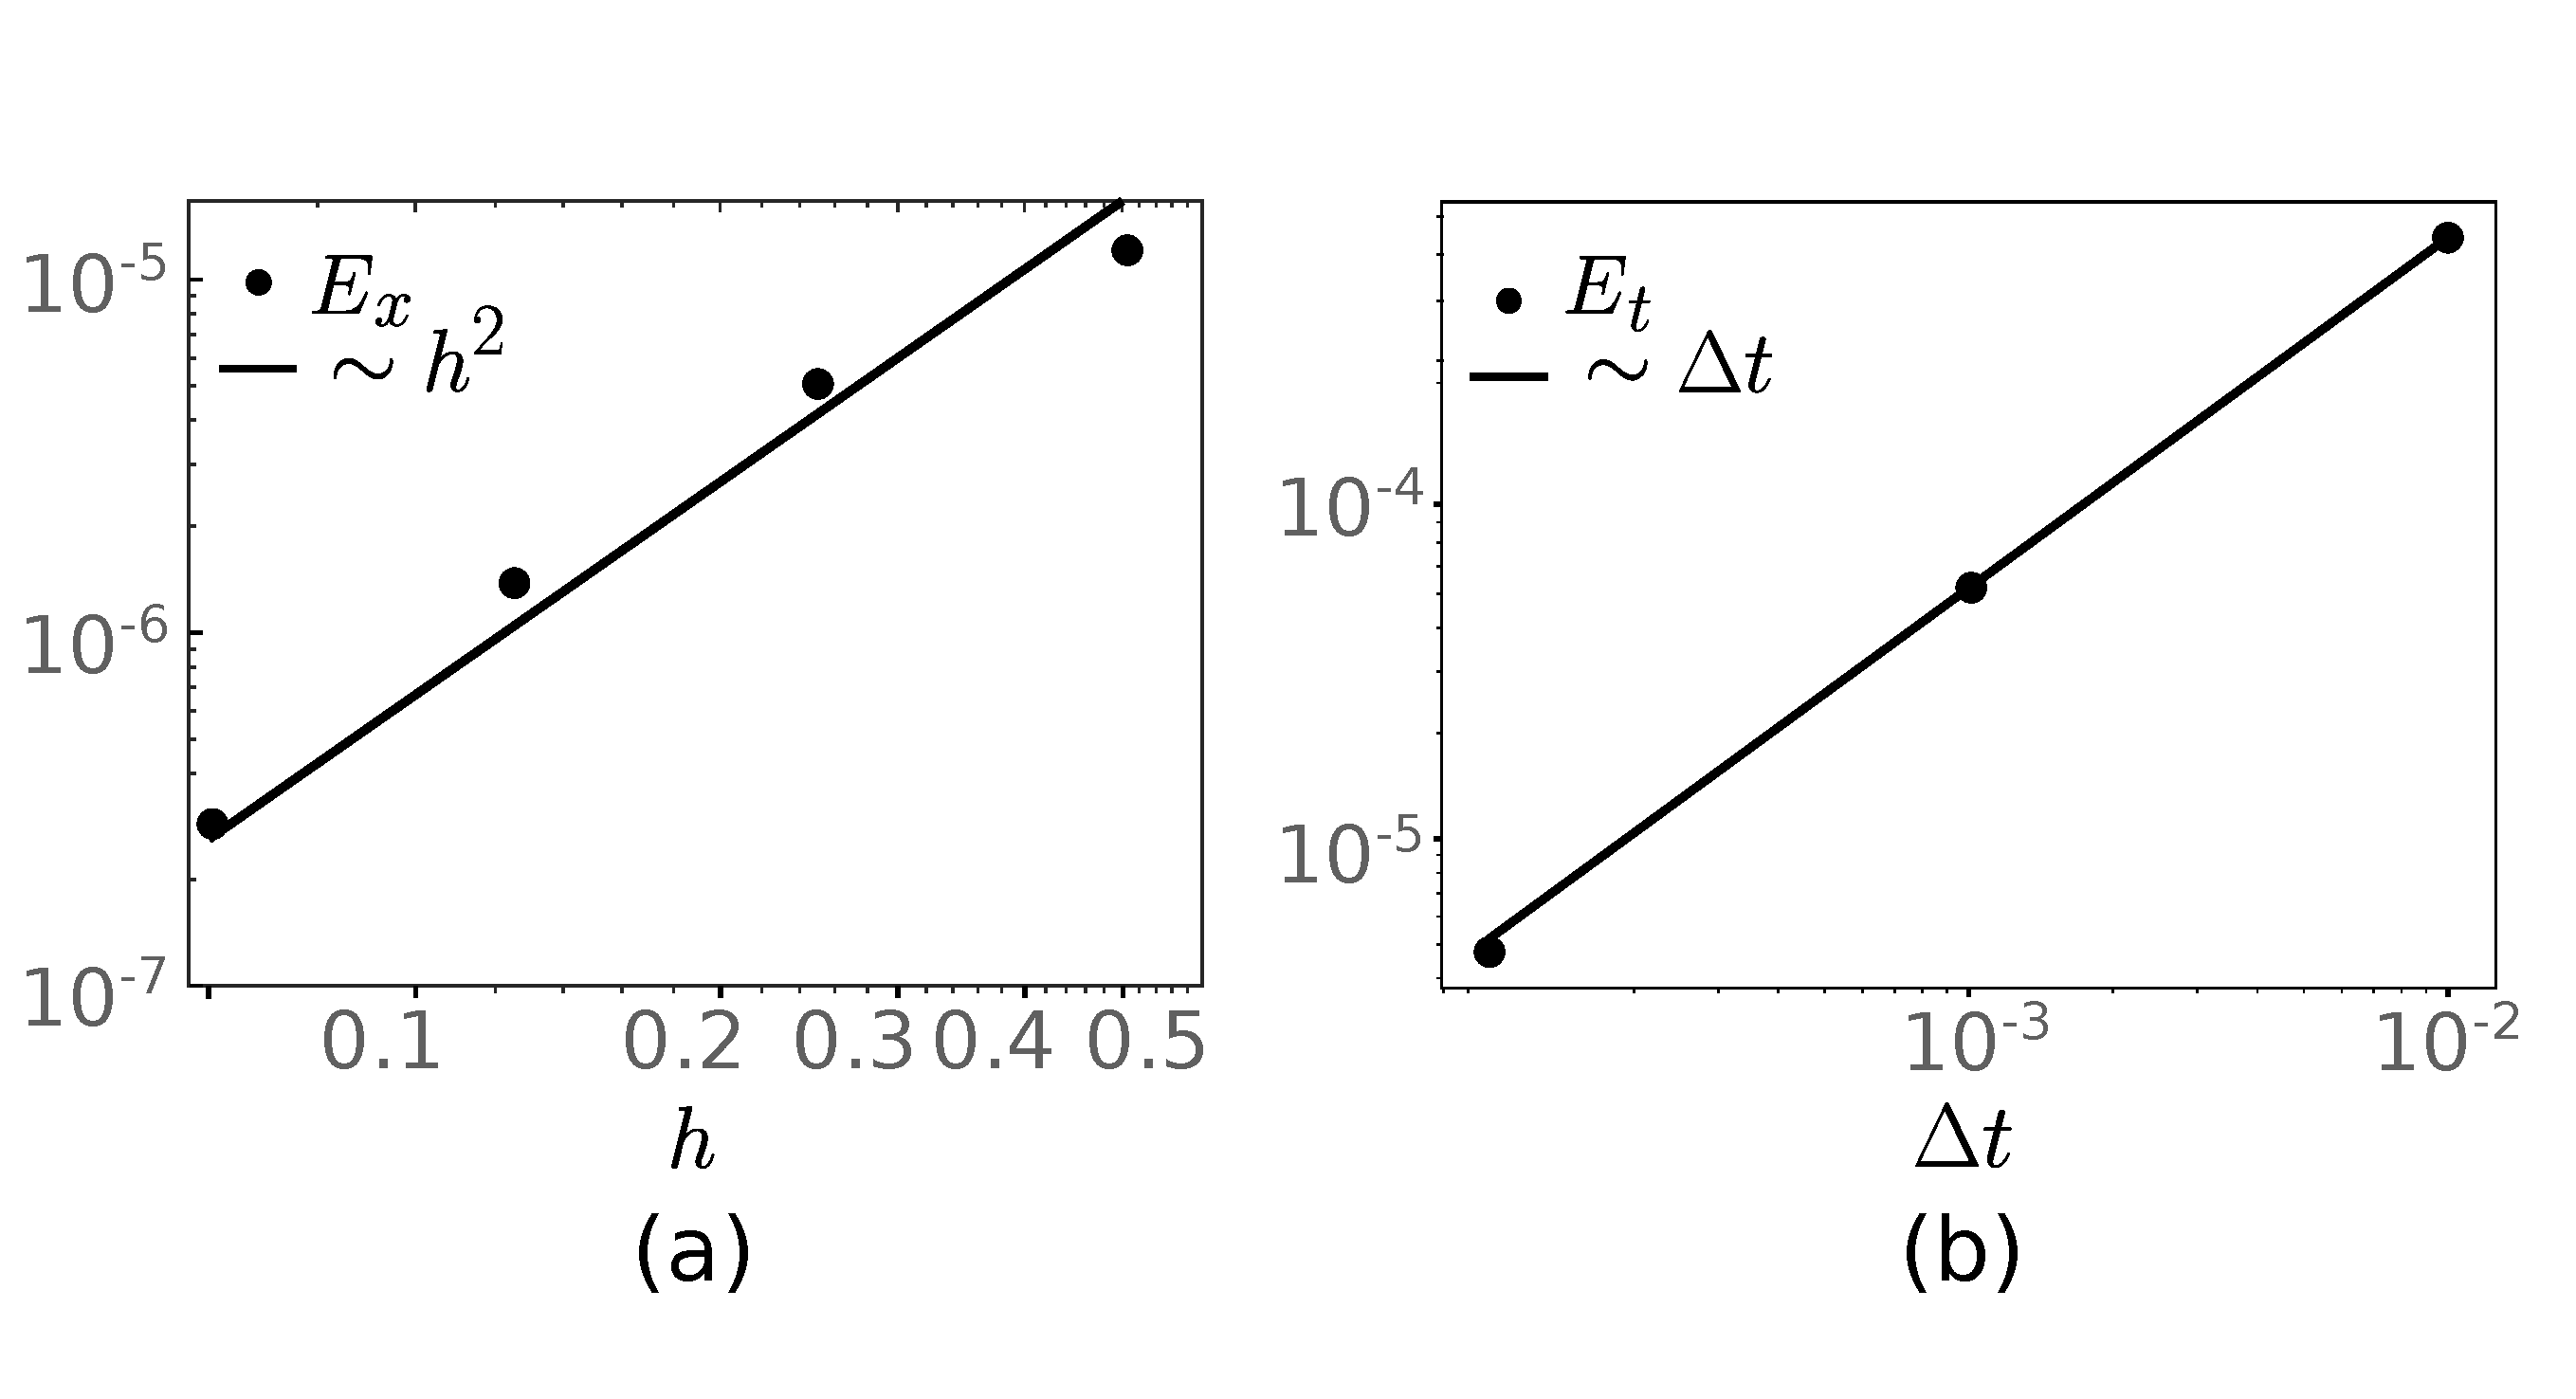
\includegraphics[width=0.9\textwidth]{append.pdf}
				\caption{\label{grid} Convergence of the numerical method. (a) Convergence of the spatial discretization. The relative free-energy error $E_x$  shows a convergence rate $\sim h^{2}$. (b) Convergence of the temporal discretization. The relative free-energy error  $E_t$  shows a convergence rate $\sim \Delta t$.}
			\end{figure}
			
			\section{Parameters used for the numerical studies}
			
			
			\begin{table}[H]
				\scriptsize
				\begin{tabular}{l|cc} \textbf{Params.} &  Fig.~\ref{sec_1_chap_3_fig_1}    &  Fig.~\ref{sec_1_chap_3_fig_2}                \\ \hline 
					$\rho_0$ [\si{\micro \meter}]  & 0.2 & 0.2  \\ 
					$\eta$ [\si{\pascal \second}] & $10^4$ & $10^4$  \\ 
					$\ell_s = \sqrt{\eta/\gamma}$ [\si{\micro \meter]} &10 &10 \\
					$k_d$ [\si{\second}$^{-1}$] &0.1 & 0.1 \\
					$D$ [\si{\micro \meter}$^2$ s$^{-1}$] & 0.02& 0.02  \\
					$\eta_{\rm rot} / \eta$ & 1&1 \\
					$\beta / \eta$ & -1 & -1,-0.1  \\
					$a/\eta$ $[\si{\second}^{-1}]$ & 1 &1   \\
					$b/\eta$ $[\si{\second}^{-1}]$  &4 &4   \\
					$L/\eta$ $[\si{\micro \meter}^2  \si{\second}^{-1}$] & $ 0.01$&$ 0.01$   \\
					$\rho_0 \lambda_{\bigodot}^0 /(2a)$ &0.4  &0.2,0.4,0.6    \\
					$\lambda^0/\eta \, [\si{\second}^{-1}]$ &0.12& 0.12  \\
					$\delta \lambda/ \lambda$   & 5& 5\\
					$\kappa = \lambda_{\rm aniso}/\lambda$  & [0.5,2]  &1.0      \\
					$\ell_0 $  [\si{\micro \meter}]  & 20  & 20  \\
					$$ [\si{\micro \meter}] & &   \\
					$\ell_p = \sqrt{L/(2|a|-\rho_0\lambda_{\odot})}$   & 0.056 &  0.0527,0.056,0.06   \\
					$$ [\si{\micro \meter}] & &    \\
					\hline
				\end{tabular}
				\caption{Parameters used in the cell wound healing study.}
				\label{modal_parameters_cell_healing}
			\end{table}
			
			\begin{table}[H]
				\scriptsize
				\begin{tabular}{l|cc} \textbf{Params.}       &  Fig.~\ref{sec_1_chap_3_fig_3}      &  Fig.~\ref{sec_1_chap_3_fig_3.5}         \\ \hline 
					$\eta$ [\si{\pascal \second}]  & $10^4$ & $10^4$  \\ 
					$\ell_s/\ell_0 = \sqrt{\eta/(\gamma \ell_0^2)}$  &10 &10 \\
					$\eta_{\rm rot} / \eta$ & 1&1\\
					$\beta / \eta$ & -0.2 & -0.2 \\
					$a/\eta$ $[\si{\second}^{-1}]$& -1 &-1 \\
					$b/\eta$ $[\si{\second}^{-1}]$   & 2 &2  \\
					$L/(\eta \ell_0^2)$ $[ \si{\second}^{-1}$] & [$8 \times 10^{-4}$ ,$0.18  $ ] & $8 \times 10^{-4}$  \\
					$\lambda_{\rm aniso}/\eta [s^{-1}]$    & 0 &$8.9 \times 10^{-3}$, $0.036$,$0.08$,$0.32$     \\
					$\ell_a / \ell_0 = \sqrt{L/\left(\lambda_{\rm aniso}S_0\right)}$   & $\infty$  & $\infty, 0.3,0.15,0.1,0.05,0.04$ \\
					$\ell_p / \ell_0 = \sqrt{L/2|a|}$   &  [0.02, 0.3]  & 0.02 \\
					\hline
				\end{tabular}
				\caption{Parameters used in the confined cell colony study.}
				\label{modal_parameters_cell_colony}
			\end{table}
			
			
			\section{Movie captions}
			\qquad 	\textbf{Movie 1} \quad Dynamics during wound healing  for various degrees of anisotropic activity quantified by $\kappa$. The density and nematic fields are represented by colormaps. The direction and length of black arrows indicate direction and magnitude of the velocity field $\bm{v}$. The direction and length of red segments indicate the average molecular orientation $\bm{n}$ and the nematic order $S$.
			
			\textbf{Movie 2} \quad Effect of activity (quantified by the ratio between the active nematic length-scale $\ell_a$ and system size $\ell_0$)  on flows and defect structure and dynamics in a confined active nematic system.  The velocity modulus and nematic fields are represented by colormaps. The direction and length of black arrows indicate direction and magnitude of the velocity field $\bm{v}$. The direction and length of red segments indicate the average molecular orientation $\bm{n}$ and the nematic order $S$.
			
			\textbf{Movie 3} \quad	 Low Reynolds number active turbulence at high activity (quantified by the ratio between the active nematic length-scale $\ell_a$ and system size $\ell_0$).  The velocity modulus and nematic fields are represented by colormaps. The direction and length of black arrows indicate direction and magnitude of the velocity field $\bm{v}$. The direction and length of red segments indicate the average molecular orientation $\bm{n}$ and the nematic order $S$.
			
			\section*{Bibliography}
			
			\begin{thebibliography}{100}
			\expandafter\ifx\csname url\endcsname\relax
				\def\url#1{{\tt #1}}\fi
			\expandafter\ifx\csname urlprefix\endcsname\relax\def\urlprefix{URL }\fi
			\providecommand{\eprint}[2][]{\url{#2}}
				% Bibliography created with iopart-num v2.1
				% /biblio/bibtex/contrib/iopart-num
				
				\bibitem{marchetti2013}
				Marchetti M~C, Joanny J~F, Ramaswamy S, Liverpool T~B, Prost J, Rao M and Simha
				  R~A 2013 {\em Reviews of modern physics\/} {\bf 85} 1143
				
				\bibitem{doostmohammadi2018}
				Doostmohammadi A, Ign{\'e}s-Mullol J, Yeomans J~M and Sagu{\'e}s F 2018 {\em
				  Nature Communications\/} {\bf 9} 1--13
				
				\bibitem{decamp2015}
				DeCamp S~J, Redner G~S, Baskaran A, Hagan M~F and Dogic Z 2015 {\em Nature
				  materials\/} {\bf 14} 1110--1115
				
				\bibitem{lemma2021}
				Lemma L~M, Norton M~M, Tayar A~M, DeCamp S~J, Aghvami S~A, Fraden S, Hagan M~F
				  and Dogic Z 2021 {\em Physical Review Letters\/} {\bf 127}(14) 148001
				
				\bibitem{li2017}
				Li J, Biel T, Lomada P, Yu Q and Kim T 2017 {\em Soft Matter\/} {\bf 13}
				  3213--3220
				
				\bibitem{yu2018}
				Yu Q, Li J, Murrell M~P and Kim T 2018 {\em Biophysical Journal\/} {\bf 115}
				  2003--2013 ISSN 0006-3495
				
				\bibitem{lehtimaki2021}
				Lehtim{\"a}ki J~I, Rajakyl{\"a} E~K, Tojkander S and Lappalainen P 2021 {\em
				  eLife\/} {\bf 10} e60710 ISSN 2050-084X
				
				\bibitem{tee2015}
				Tee Y~H, Shemesh T, Thiagarajan V, Hariadi R~F, Anderson K~L, Page C, Volkmann
				  N, Hanein D, Sivaramakrishnan S, Kozlov M~M {\em et~al.\/} 2015 {\em Nature
				  Cell Biology\/} {\bf 17} 445--457
				
				\bibitem{tojkander2015}
				Tojkander S, Gateva G, Husain A, Krishnan R and Lappalainen P 2015 {\em
				  eLife\/} {\bf 4} e06126
				
				\bibitem{wirshing2017}
				Wirshing A~C and Cram E~J 2017 {\em Molecular Biology of the Cell (MBoC)\/}
				  {\bf 28} 1937--1949
				
				\bibitem{yolland2019}
				Yolland L, Burki M, Marcotti S, Luchici A, Kenny F~N, Davis J~R, Serna-Morales
				  E, M{\"u}ller J, Sixt M, Davidson A {\em et~al.\/} 2019 {\em Nature Cell
				  Biology\/} {\bf 21} 1370--1381
				
				\bibitem{jalal2019}
				Jalal S, Shi S, Acharya V, Huang R~Y~J, Viasnoff V, Bershadsky A~D and Tee Y~H
				  2019 {\em Journal of Cell Science\/} {\bf 132} jcs220780
				
				\bibitem{weirich2017}
				Weirich K~L, Banerjee S, Dasbiswas K, Witten T~A, Vaikuntanathan S and Gardel
				  M~L 2017 {\em Proceedings of the National Academy of Sciences\/} {\bf 114}
				  2131--2136
				
				\bibitem{weirich2019}
				Weirich K~L, Dasbiswas K, Witten T~A, Vaikuntanathan S and Gardel M~L 2019 {\em
				  Proceedings of the National Academy of Sciences\/} {\bf 116} 11125--11130
				
				\bibitem{wioland2013}
				Wioland H, Woodhouse F~G, Dunkel J, Kessler J~O and Goldstein R~E 2013 {\em
				  Physical Review Letters\/} {\bf 110}(26) 268102
				
				\bibitem{duclos2017}
				Duclos G, Erlenk{\"a}mper C, Joanny J~F and Silberzan P 2017 {\em Nature
				  Physics\/} {\bf 13} 58--62
				
				\bibitem{guillamat2020}
				Guillamat P, Blanch-Mercader C, Pernollet G, Kruse K and Roux A 2022 {\em
				  Nature Materials\/} {\bf 21} 588--597
				
				\bibitem{doxzen2013}
				Doxzen K, Vedula S~R~K, Leong M~C, Hirata H, Gov N~S, Kabla A~J, Ladoux B and
				  Lim C~T 2013 {\em Integrative Biology\/} {\bf 5} 1026--1035 ISSN 1757-9708
				
				\bibitem{callan2013}
				Callan-Jones A and Voituriez R 2013 {\em New Journal of Physics\/} {\bf 15}
				  025022
				
				\bibitem{Ruprecht:2015aa}
				Ruprecht V, Wieser S, Callan-Jones A, Smutny M, Morita H, Sako K, Barone V,
				  Ritsch-Marte M, Sixt M, Voituriez R and Heisenberg C~P 2015 {\em Cell\/} {\bf
				  160} 673--685
				
				\bibitem{hannezo2015}
				Hannezo E, Dong B, Recho P, Joanny J~F and Hayashi S 2015 {\em Proceedings of
				  the National Academy of Sciences\/} {\bf 112} 8620--8625
				
				\bibitem{opathalage2019}
				Opathalage A, Norton M~M, Juniper M~P~N, Langeslay B, Aghvami S~A, Fraden S and
				  Dogic Z 2019 {\em Proceedings of the National Academy of Sciences\/} {\bf
				  116} 4788--4797
				
				\bibitem{gao2017}
				Gao T, Betterton M~D, Jhang A~S and Shelley M~J 2017 {\em Physical Review Fluids\/}
				  {\bf 2}(9) 093302
				
				\bibitem{xia2019}
				Xia S, Lim Y~B, Zhang Z, Wang Y, Zhang S, Lim C~T, Yim E~K and Kanchanawong P
				  2019 {\em Cell Reports\/} {\bf 28} 1251--1267
				
				\bibitem{mirza2022}
				Mirza W, Corato M~D, Pensalfini M, Vilanova G, Torres-S\'anchez A and Arroyo M
				  2022 {\em TBA\/}
				
				\bibitem{bechinger2016}
				Bechinger C, Di~Leonardo R, L{\"o}wen H, Reichhardt C, Volpe G and Volpe G 2016
				  {\em Reviews of Modern Physics\/} {\bf 88} 045006
				
				\bibitem{patelli2019}
				Patelli A, Djafer-Cherif I, Aranson I~S, Bertin E and Chat{\'e} H 2019 {\em
				  Physical review letters\/} {\bf 123} 258001
				
				\bibitem{alaimo2017}
				Alaimo F, K{\"o}hler C and Voigt A 2017 {\em Scientific reports\/} {\bf 7} 1--9
				
				\bibitem{ehrig2017}
				Ehrig S, Ferracci J, Weinkamer R and Dunlop J~W~C 2017 {\em Physical Review E\/}
				  {\bf 95}(6) 062609
				
				\bibitem{keber2014}
				Keber F~C, Loiseau E, Sanchez T, DeCamp S~J, Giomi L, Bowick M~J, Marchetti
				  M~C, Dogic Z and Bausch A~R 2014 {\em Science\/} {\bf 345} 1135--1139
				
				\bibitem{khoromskaia2017}
				Khoromskaia D and Alexander G~P 2017 {\em New Journal of Physics\/} {\bf 19}
				  103043
				
				\bibitem{ellis2018}
				Ellis P~W, Pearce D~J, Chang Y~W, Goldsztein G, Giomi L and Fernandez-Nieves A
				  2018 {\em Nature Physics\/} {\bf 14} 85--90
				
				\bibitem{mandato2001}
				Mandato C~A and Bement W~M 2001 {\em The Journal of cell biology\/} {\bf 154}
				  785--798
				
				\bibitem{anne2016}
				Reymann A~C, Staniscia F, Erzberger A, Salbreux G and Grill S~W 2016 {\em
				  eLife\/} {\bf 5} e17807 ISSN 2050-084X
				
				\bibitem{vcopar2019}
				\ifmmode~\check{C}\else \v{C}\fi{}opar S, Aplinc J, Kos i~c~v,
				  \ifmmode~\check{Z}\else \v{Z}\fi{}umer S and Ravnik M 2019 {\em Physical Review
				  X\/} {\bf 9}(3) 031051
				
				\bibitem{zhang2020}
				Zhang Y~H, Deserno M, Tu Z~C {\em et~al.\/} 2020 {\em Physical Review E\/} {\bf
				  102} 012607
				
				\bibitem{napoli2020}
				Napoli G and Turzi S 2020 {\em Physical Review E\/} {\bf 101} 022701
				
				\bibitem{pearce2020}
				Pearce D~J~G 2020 {\em New Journal of Physics\/} {\bf 22} 063051
				
				\bibitem{nestler2018}
				Nestler M, Nitschke I, Praetorius S and Voigt A 2018 {\em Journal of Nonlinear
				  Science\/} {\bf 28} 147--191
				
				\bibitem{hemingway2016}
				Hemingway E~J, Mishra P, Marchetti M~C and Fielding S~M 2016 {\em Soft
				  Matter\/} {\bf 12}(38) 7943--7952
				
				\bibitem{julicher2018}
				J{\"u}licher F, Grill S~W and Salbreux G 2018 {\em Reports on Progress in
				  Physics\/} {\bf 81} 076601
				
				\bibitem{metselaar2019}
				Metselaar L, Yeomans J~M and Doostmohammadi A 2019 {\em Physical Review Letters\/}
				  {\bf 123}(20) 208001
				
				\bibitem{simha2002}
				Simha R~A and Ramaswamy S 2002 {\em Physical Review Letters\/} {\bf 89} 058101
				
				\bibitem{hatwalne2004}
				Hatwalne Y, Ramaswamy S, Rao M and Simha R~A 2004 {\em Physical Review Letters\/} {\bf
				  92}(11) 118101
				
				\bibitem{salbreux2022}
				Salbreux G, J\"ulicher F, Prost J and Callan-Jones A 2022 {\em Physical Review
				  Research\/} {\bf 4}(3) 033158
				
				\bibitem{baskaran2008}
				Baskaran A and Marchetti M~C 2008 {\em Physical Review E\/} {\bf 77}(1) 011920
				
				\bibitem{bertin2013}
				Bertin E, Chat{\'{e}} H, Ginelli F, Mishra S, Peshkov A and Ramaswamy S 2013
				  {\em New Journal of Physics\/} {\bf 15} 085032
				
				\bibitem{peshkov2012}
				Peshkov A, Aranson I~S, Bertin E, Chat\'e H and Ginelli F 2012 {\em Physical Review
				  Lett.\/} {\bf 109}(26) 268701
				
				\bibitem{marenduzzo2007}
				Marenduzzo D, Orlandini E, Cates M~E and Yeomans J~M 2007 {\em Physical Review E\/}
				  {\bf 76}(3) 031921
				
				\bibitem{cates2009}
				Cates M~E, Henrich O, Marenduzzo D and Stratford K 2009 {\em Soft Matter\/}
				  {\bf 5}(20) 3791--3800
				
				\bibitem{desplat2001}
				Desplat J~C, Pagonabarraga I and Bladon P 2001 {\em Computer Physics
				  Communications\/} {\bf 134} 273--290 ISSN 0010-4655
				
				\bibitem{goudiaby2021}
				Goudiaby M~S, Diagne A and Tine L~M 2021 {\em Communications on Pure and
				  Applied Analysis\/} {\bf 20} 3499--3514 ISSN 1534-0392
				
				\bibitem{becker2008}
				Becker R, Feng X and Prohl A 2008 {\em SIAM Journal on Numerical Analysis\/}
				  {\bf 46} 1704--1731
				
				\bibitem{norton2018}
				Norton M~M, Baskaran A, Opathalage A, Langeslay B, Fraden S, Baskaran A and
				  Hagan M~F 2018 {\em Physical Review E\/} {\bf 97}(1) 012702
				
				\bibitem{benink2000}
				Benink H~A, Mandato C~A and Bement W~M 2000 {\em Molecular Biology of the
				  Cell\/} {\bf 11} 2553--2563 pMID: 10930453
				
				\bibitem{duclos2014}
				Duclos G, Garcia S, Yevick H~G and Silberzan P 2014 {\em Soft Matter\/} {\bf
				  10}(14) 2346--2353
				
				\bibitem{de2013non}
				De~Groot S and Mazur P 2013 {\em Non-Equilibrium Thermodynamics\/} Dover Books
				  on Physics (Dover Publications) ISBN 9780486153506
				
				\bibitem{kondepudi2014modern}
				Kondepudi D and Prigogine I 2014 {\em Modern Thermodynamics: From Heat Engines
				  to Dissipative Structures\/} CourseSmart Series (Wiley) ISBN 9781118371817
				
				\bibitem{Prost:2015aa}
				Prost J, J{\"u}licher F and Joanny J~F 2015 {\em Nature Physics\/} {\bf 11}
				  111--117
				
				\bibitem{Onsager1931}
				Onsager L 1931 {\em Physical Review\/} {\bf 37}(4) 405--426
				
				\bibitem{PhysRev.38.2265}
				Onsager L 1931 {\em Physical Review\/} {\bf 38}(12) 2265--2279
				
				\bibitem{Coleman:1963aa}
				Coleman B~D and Noll W 1963 {\em Archive for Rational Mechanics and Analysis\/}
				  {\bf 13} 167--178
				
				\bibitem{Coleman_Gurtin}
				Coleman B~D and Gurtin M~E 2004 {\em The Journal of Chemical Physics\/} {\bf
				  47} 597--613 ISSN 0021-9606
				
				\bibitem{ZIEGLER1987183}
				Ziegler H and Wehrli C 1987 The derivation of constitutive relations from the
				  free energy and the dissipation function ({\em Advances in Applied
				  Mechanics\/} vol~25) ed Wu T~Y and Hutchinson J~W (Elsevier) pp 183--238
				
				\bibitem{Maugin}
				Maugin G~A 1999 {\em The Thermomechanics of Nonlinear Irreversible Behaviors\/}
				  (WORLD SCIENTIFIC)
				
				\bibitem{rayleigh1873}
				Rayleigh L 1873 {\em Proc. Math Soc. London\/} {\bf 363}
				
				\bibitem{PhysRev.91.1505}
				Onsager L and Machlup S 1953 {\em Physical Review\/} {\bf 91}(6) 1505--1512
				
				\bibitem{peletier2014variational}
				Peletier M~A 2014 Variational modelling: Energies, gradient flows, and large
				  deviations
				
				\bibitem{D0SM02076A}
				Wang H, Qian T and Xu X 2021 {\em Soft Matter\/} {\bf 17}(13) 3634--3653
				
				\bibitem{Gyarmati}
				Gyarmati I 1970 {\em Non-equilibrium Thermodynamics: Field Theory and
				  Variational Principles\/} (Springer Berlin, Heidelberg)
				
				\bibitem{BIOT19841}
				Biot M 1984 New variational-lagrangian irreversible thermodynamics with
				  application to viscous flow, reaction--diffusion, and solid mechanics ({\em
				  Advances in Applied Mechanics\/} vol~24) ed Hutchinson J~W and Wu T~Y
				  (Elsevier) pp 1--91
				
				\bibitem{PhysRev.97.1463}
				Biot M~A 1955 {\em Physical Review\/} {\bf 97}(6) 1463--1469
				
				\bibitem{EDELEN1972481}
				Edelen D~G 1972 {\em International Journal of Engineering Science\/} {\bf 10}
				  481--490 ISSN 0020-7225
				
				\bibitem{ORTIZ1999397}
				Ortiz M and Repetto E 1999 {\em Journal of the Mechanics and Physics of
				  Solids\/} {\bf 47} 397--462 ISSN 0022-5096
				
				\bibitem{Mielke:2003aa}
				Mielke A 2003 {\em Continuum Mechanics and Thermodynamics\/} {\bf 15} 351--382
				
				\bibitem{mielke2016generalization}
				Mielke A, Renger D~R~M and Peletier M~A 2016 {\em Journal of Non-Equilibrium
				  Thermodynamics\/} {\bf 41} 141--149
				
				\bibitem{MIEHE20022123}
				Miehe C, Schotte J and Lambrecht M 2002 {\em Journal of the Mechanics and
				  Physics of Solids\/} {\bf 50} 2123--2167 ISSN 0022-5096
				
				\bibitem{doi2011}
				Doi M 2011 {\em Journal of Physics: Condensed Matter\/} {\bf 23} 284118
				
				\bibitem{arroyo2009}
				Arroyo M and DeSimone A 2009 {\em Physical Review E\/} {\bf 79}(3) 031915
				
				\bibitem{arroyo2018}
				Arroyo M, Walani N, Torres-S{\'a}nchez A and Kaurin D 2018 {\em Onsager's
				  Variational Principle in Soft Matter: Introduction and Application to the
				  Dynamics of Adsorption of Proteins onto Fluid Membranes\/} (Cham: Springer
				  International Publishing) pp 287--332 ISBN 978-3-319-56348-0
				
				\bibitem{kaurin-bal}
				Kaurin D, Bal P~K and Arroyo M 2022 {\em Journal of The Royal Society
				  Interface\/} {\bf 19} 20220183
				
				\bibitem{Tozzi_2019}
				Tozzi C, Walani N and Arroyo M 2019 {\em New Journal of Physics\/} {\bf 21}
				  093004
				
				\bibitem{10.1122/8.0000475}
				De~Corato M and Arroyo M 2022 {\em Journal of Rheology\/} {\bf 66} 813--835
				  ISSN 0148-6055
				
				\bibitem{Otto2001}
				Otto F 2001 {\em Communications in Partial Differential Equations\/} {\bf 26}
				  101--174
				
				\bibitem{torres2019}
				Torres-S{\'a}nchez A, Mill{\'a}n D and Arroyo M 2019 {\em Journal of Fluid
				  Mechanics\/} {\bf 872} 218--271
				
				\bibitem{Noselli:2019aa}
				Noselli G, Beran A, Arroyo M and DeSimone A 2019 {\em Nature Physics\/} {\bf
				  15} 496--502
				
				\bibitem{turlier2014}
				Turlier H, Audoly B, Prost J and Joanny J~F 2014 {\em Biophysical journal\/}
				  {\bf 106} 114--123
				
				\bibitem{PhysRevLett.127.110601}
				Goychuk I and P\"oschel T 2021 {\em Physical Review Letters\/} {\bf 127}(11) 110601
				
				\bibitem{sens-PNAS}
				Sens P 2020 {\em Proceedings of the National Academy of Sciences\/} {\bf 117}
				  24670--24678
				
				\bibitem{de1993}
				de~Gennes P and Prost J 1993 {\em The Physics of Liquid Crystals\/}
				  International Series of Monogr (Clarendon Press) ISBN 9780198517856
				
				\bibitem{marsden1994}
				Marsden J~E and Hughes T~J 1994 {\em Mathematical foundations of elasticity\/}
				  (Courier Corporation)
				
				\bibitem{Alexander}
				Mielke A 2013 Thermomechanical modeling of energy-reaction-diffusion systems,
				  including bulk-interface interactions
				
				\bibitem{mirza2023}
				Mirza W, Vilanova G, S{\'a}nchez A~T and Arroyo M 2023 {\em TBA\/}
				
				\bibitem{waleed_thesis}
				Mirza W~A 2023 {\em A theoretical and computational study of the active
				  self-organization of nematic patterns in thin cytoskeletal layers and their
				  effect on curvature\/} Ph.D. thesis Universitat Polit{\`e}cnica de Catalunya
				
				\bibitem{cosserat1896theorie}
				Altenbach J, Altenbach H and Eremeyev V~A 2010 {\em Archive of Applied
				  Mechanics\/} {\bf 80} 73--92
				
				\bibitem{salbreux2009}
				Salbreux G, Prost J and Joanny J~F 2009 {\em Physical Review Letters\/} {\bf
				  103} 058102
				
				\bibitem{Onsager_shape}
				Onsager L 1949 {\em Annals of the New York Academy of Sciences\/} {\bf 51}
				  627--659
				
				\bibitem{D0SM01733G}
				Tozzi C, Walani N, Le~Roux A~L, Roca-Cusachs P and Arroyo M 2021 {\em Soft
				  Matter\/} {\bf 17}(12) 3367--3379
				
				\bibitem{donea2003}
				Donea J and Huerta A 2003 {\em Finite element methods for flow problems\/}
				  (John Wiley \& Sons)
				
				\bibitem{Alice2008}
				Rodriguez‐Diaz A, Toyama Y, Abravanel D~L, Wiemann J~M, Wells A~R, Tulu U~S,
				  Edwards G~S and Kiehart D~P 2008 {\em HFSP Journal\/} {\bf 2} 220--237 pMID:
				  19404432
				
				\bibitem{antiga2008}
				Antiga L, Piccinelli M, Botti L, Ene-Iordache B, Remuzzi A and Steinman D~A
				  2008 {\em Medical \& biological engineering \& computing\/} {\bf 46}
				  1097--1112
				
				\bibitem{schroeder2003}
				Schroeder W, Martin K and Lorensen B 2003 The visualization toolkit, 3rd edn.
				  kitware
				
				\bibitem{elsdale1968}
				Elsdale T 1968 {\em Experimental Cell Research\/} {\bf 51} 439--450 ISSN
				  0014-4827
				
				\bibitem{jubin2009}
				Jubin B 2009 A generalized poincar{\'e}-hopf index theorem arXiv
				
				\bibitem{hardouin2019}
				Hardo{\"u}in J, Hughes R, Doostmohammadi A, Laurent J, Lopez-Leon T, Yeomans
				  J~M, Ign{\'e}s-Mullol J and Sagu{\'e}s F 2019 {\em Communications Physics\/}
				  {\bf 2} 1--9
				
				\bibitem{giomi2014}
				Giomi L, Bowick M~J, Mishra P, Sknepnek R and Cristina~Marchetti M 2014 {\em
				  Philosophical Transactions of the Royal Society A: Mathematical, Physical and
				  Engineering Sciences\/} {\bf 372} 20130365
				
				\bibitem{thijssen2020}
				Thijssen K and Doostmohammadi A 2020 {\em Physical Review Research\/} {\bf 2}(4)
				  042008
				
				\bibitem{vafa2020}
				Vafa F 2022 {\em Soft Matter\/} {\bf 18}(42) 8087--8097
				
				\bibitem{ronning2022}
				R{\o}nning J, Marchetti C~M, Bowick M~J and Angheluta L 2022 {\em Proceedings
				  of the Royal Society A\/} {\bf 478} 20210879
				
				\bibitem{chandrakar2020}
				Chandrakar P, Varghese M, Aghvami S, Baskaran A, Dogic Z and Duclos G 2020 {\em
				  Physical Review Letters\/} {\bf 125}(25) 257801
				
				\bibitem{ramaswamy2007}
				Ramaswamy S and Rao M 2007 {\em New Journal of Physics\/} {\bf 9} 423--423
				
				\bibitem{ramaswamy2010}
				Ramaswamy S 2010 {\em Annual Review of Condensed Matter Physics\/} {\bf 1}
				  323--345
				
				\bibitem{mayer2010}
				Mayer M, Depken M, Bois J~S, J{\"u}licher F and Grill S~W 2010 {\em Nature\/}
				  {\bf 467} 617--621
				
				\bibitem{maroudas2021}
				Maroudas-Sacks Y, Garion L, Shani-Zerbib L, Livshits A, Braun E and Keren K
				  2021 {\em Nature Physics\/} {\bf 17} 251--259
				
				\bibitem{doi:10.1080/00029890.1991.11995702}
				Gilbert G~T 1991 {\em The American Mathematical Monthly\/} {\bf 98} 44--46
				
				\end{thebibliography}
				
		\end{document}